\chapter{分析画像}\label{ap:analysis}

本論の構成上入りきらなかった分析画像をここに記す.

\section{ヒストグラム}

\subsection{重力と熱流を同時にかける}

図\ref{fig:RaRtmap_time}の結果をそれぞれ正規化したヒストグラムにして表す.

\begin{figure}[H]
  \begin{tabular}{ccccc}
    \begin{minipage}[t]{0.2\hsize}
      \centering
      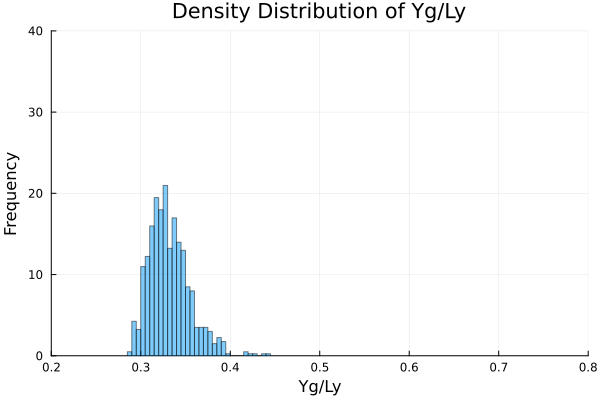
\includegraphics[width=\textwidth]{image/RaRtmap_hist/2023-11-14T18:19:29.358__chi1.265_Ay50_rho0.4_T0.43_dT0.04_Rd0.0_Rt0.0_Ra0.0_g0.0003999718779659611_run4.0e7_output.png}
      \subcaption{$\text{R}_\text{a}=0.0,\text{R}_\text{t}=0.0$}
      \label{fig:RaRtmap_hist_Ra0.0_Rt0.0}
    \end{minipage} &
    \begin{minipage}[t]{0.2\hsize}
      \centering
      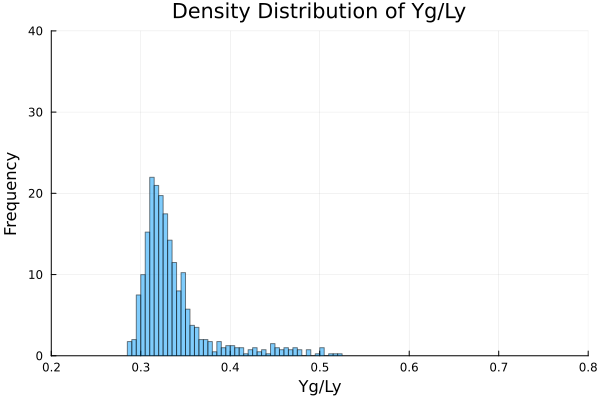
\includegraphics[width=\textwidth]{image/RaRtmap_hist/2023-11-14T19:14:52.710__chi1.265_Ay50_rho0.4_T0.43_dT0.04_Rd0.0_Rt0.0_Ra0.4693845_g0.0003999718779659611_run4.0e7_output.png}
      \subcaption{$\text{R}_\text{a}=0.469,\\\text{R}_\text{t}=0.0$}
      \label{}
    \end{minipage} &
    \begin{minipage}[t]{0.2\hsize}
      \centering
      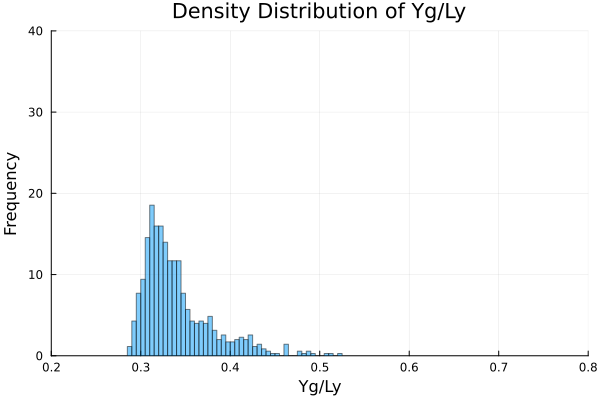
\includegraphics[width=\textwidth]{image/RaRtmap_hist/2023-11-14T20:07:58.625__chi1.265_Ay50_rho0.4_T0.43_dT0.04_Rd0.0_Rt0.0_Ra0.938769_g0.0003999718779659611_run4.0e7_output.png}
      \subcaption{$\text{R}_\text{a}=0.938,\\\text{R}_\text{t}=0.0$}
      \label{}
    \end{minipage} &
    \begin{minipage}[t]{0.2\hsize}
      \centering
      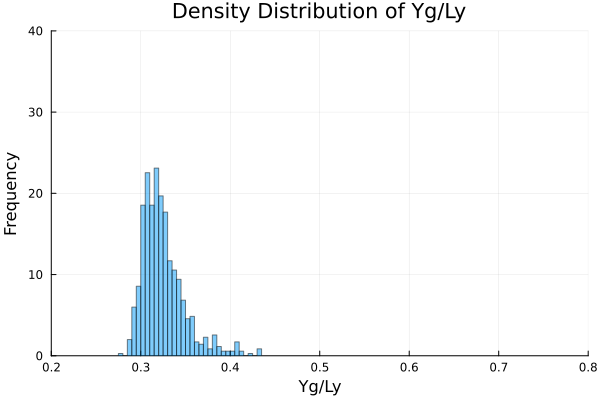
\includegraphics[width=\textwidth]{image/RaRtmap_hist/2023-11-14T21:01:09.992__chi1.265_Ay50_rho0.4_T0.43_dT0.04_Rd0.0_Rt0.0_Ra1.4081535_g0.0003999718779659611_run4.0e7_output.png}
      \subcaption{$\text{R}_\text{a}=1.408,\\\text{R}_\text{t}=0.0$}
      \label{}
    \end{minipage} &
    \begin{minipage}[t]{0.2\hsize}
      \centering
      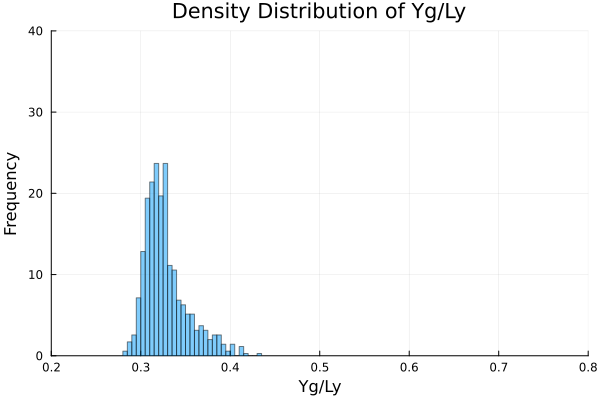
\includegraphics[width=\textwidth]{image/RaRtmap_hist/2023-11-14T21:54:59.835__chi1.265_Ay50_rho0.4_T0.43_dT0.04_Rd0.0_Rt0.0_Ra1.877538_g0.0003999718779659611_run4.0e7_output.png}
      \subcaption{$\text{R}_\text{a}=1.877,\\\text{R}_\text{t}=0.0$}
      \label{}
    \end{minipage} \\
    \begin{minipage}[t]{0.2\hsize}
      \centering
      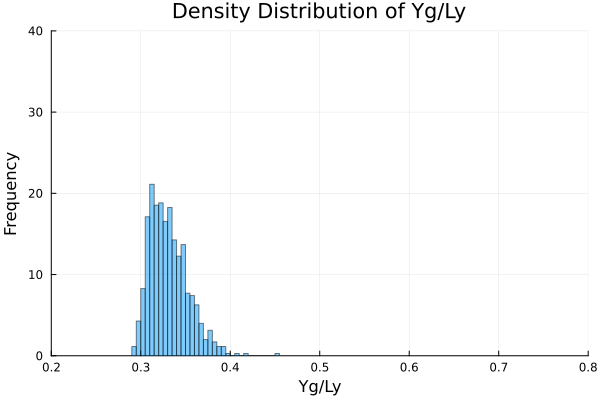
\includegraphics[width=\textwidth]{image/RaRtmap_hist/2023-11-14T22:51:24.191__chi1.265_Ay50_rho0.4_T0.43_dT0.04_Rd0.0_Rt0.125_Ra0.0_g0.0003999718779659611_run4.0e7_output.png}
      \subcaption{$\text{R}_\text{a}=0.0,\\\text{R}_\text{t}=0.125$}
      \label{}
    \end{minipage} &
    \begin{minipage}[t]{0.2\hsize}
      \centering
      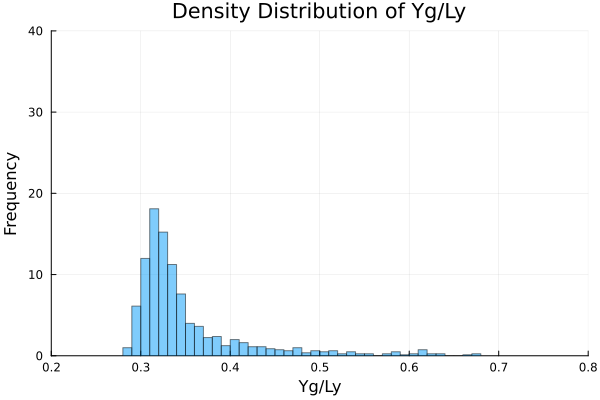
\includegraphics[width=\textwidth]{image/RaRtmap_hist/2023-11-14T23:48:31.439__chi1.265_Ay50_rho0.4_T0.43_dT0.04_Rd0.0_Rt0.125_Ra0.4693845_g0.0003999718779659611_run4.0e7_output.png}
      \subcaption{$\text{R}_\text{a}=0.469,\\\text{R}_\text{t}=0.125$}
      \label{}
    \end{minipage} &
    \begin{minipage}[t]{0.2\hsize}
      \centering
      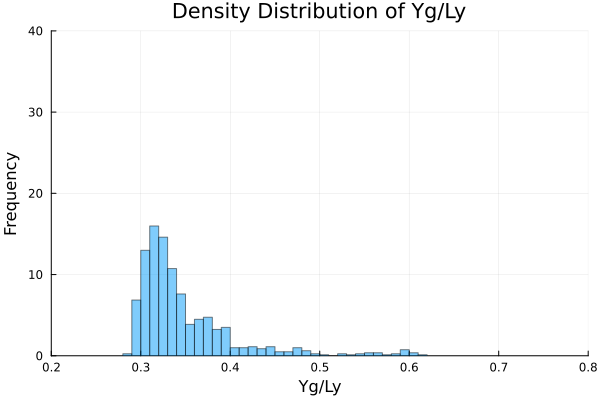
\includegraphics[width=\textwidth]{image/RaRtmap_hist/2023-11-15T00:43:33.781__chi1.265_Ay50_rho0.4_T0.43_dT0.04_Rd0.0_Rt0.125_Ra0.938769_g0.0003999718779659611_run4.0e7_output.png}
      \subcaption{$\text{R}_\text{a}=0.938,\\\text{R}_\text{t}=0.125$}
      \label{}
    \end{minipage} &
    \begin{minipage}[t]{0.2\hsize}
      \centering
      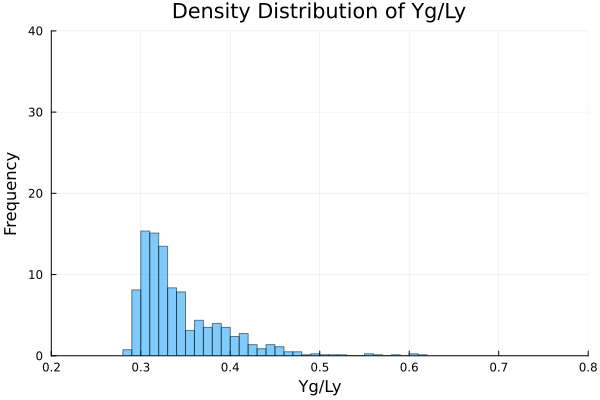
\includegraphics[width=\textwidth]{image/RaRtmap_hist/2023-11-15T01:35:17.404__chi1.265_Ay50_rho0.4_T0.43_dT0.04_Rd0.0_Rt0.125_Ra1.4081535_g0.0003999718779659611_run4.0e7_output.png}
      \subcaption{$\text{R}_\text{a}=1.408,\\\text{R}_\text{t}=0.125$}
      \label{}
    \end{minipage} &
    \begin{minipage}[t]{0.2\hsize}
      \centering
      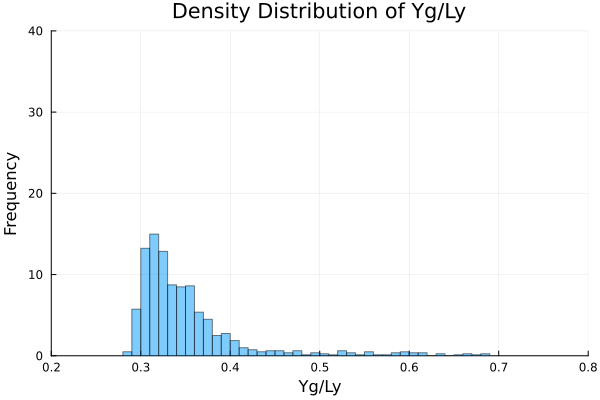
\includegraphics[width=\textwidth]{image/RaRtmap_hist/2023-11-15T02:27:34.337__chi1.265_Ay50_rho0.4_T0.43_dT0.04_Rd0.0_Rt0.125_Ra1.877538_g0.0003999718779659611_run4.0e7_output.png}
      \subcaption{$\text{R}_\text{a}=1.877,\\\text{R}_\text{t}=0.125$}
      \label{}
    \end{minipage} \\
    \begin{minipage}[t]{0.2\hsize}
      \centering
      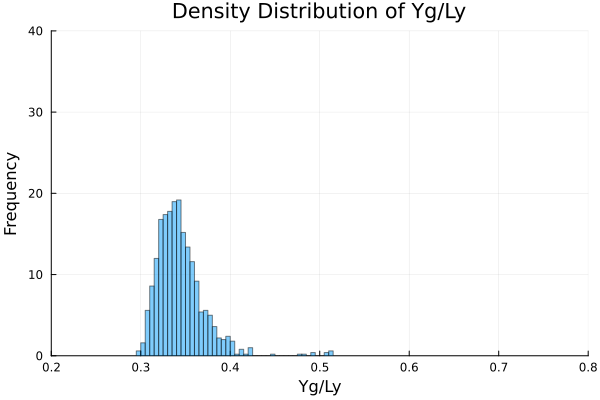
\includegraphics[width=\textwidth]{image/RaRtmap_hist/2023-11-15T03:19:32.715__chi1.265_Ay50_rho0.4_T0.43_dT0.04_Rd0.0_Rt0.25_Ra0.0_g0.0003999718779659611_run4.0e7_output.png}
      \subcaption{$\text{R}_\text{a}=0.0,\\\text{R}_\text{t}=0.250$}
      \label{}
    \end{minipage} &
    \begin{minipage}[t]{0.2\hsize}
      \centering
      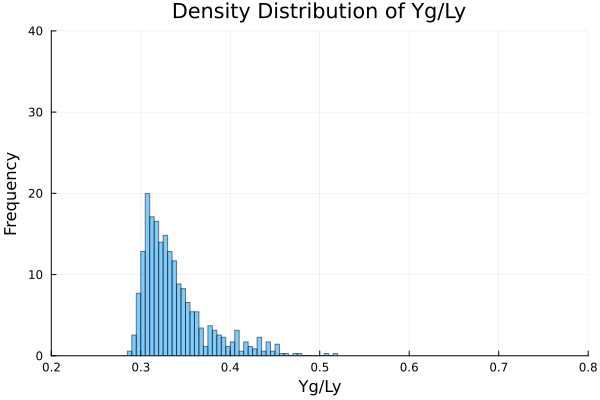
\includegraphics[width=\textwidth]{image/RaRtmap_hist/2023-11-15T04:11:00.956__chi1.265_Ay50_rho0.4_T0.43_dT0.04_Rd0.0_Rt0.25_Ra0.4693845_g0.0003999718779659611_run4.0e7_output.png}
      \subcaption{$\text{R}_\text{a}=0.469,\\\text{R}_\text{t}=0.250$}
      \label{}
    \end{minipage} &
    \begin{minipage}[t]{0.2\hsize}
      \centering
      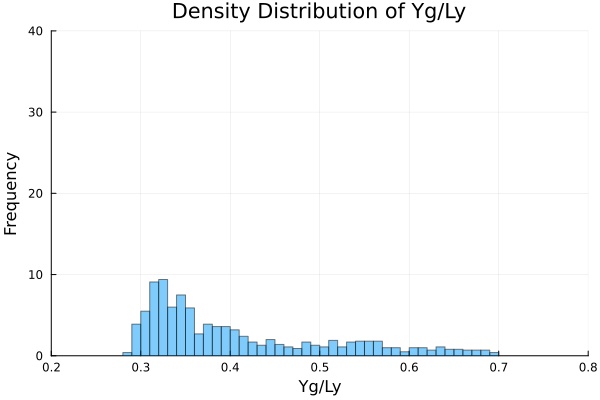
\includegraphics[width=\textwidth]{image/RaRtmap_hist/2023-11-15T05:03:45.973__chi1.265_Ay50_rho0.4_T0.43_dT0.04_Rd0.0_Rt0.25_Ra0.938769_g0.0003999718779659611_run4.0e7_output.png}
      \subcaption{$\text{R}_\text{a}=0.938,\\\text{R}_\text{t}=0.250$}
      \label{}
    \end{minipage} &
    \begin{minipage}[t]{0.2\hsize}
      \centering
      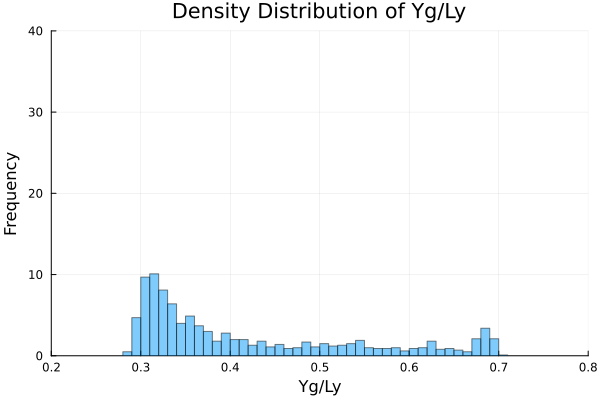
\includegraphics[width=\textwidth]{image/RaRtmap_hist/2023-11-15T05:53:00.667__chi1.265_Ay50_rho0.4_T0.43_dT0.04_Rd0.0_Rt0.25_Ra1.4081535_g0.0003999718779659611_run4.0e7_output.png}
      \subcaption{$\text{R}_\text{a}=1.408,\\\text{R}_\text{t}=0.250$}
      \label{}
    \end{minipage} &
    \begin{minipage}[t]{0.2\hsize}
      \centering
      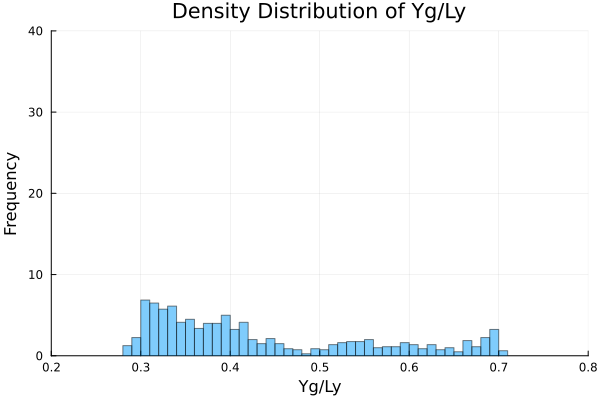
\includegraphics[width=\textwidth]{image/RaRtmap_hist/2023-11-15T06:43:21.554__chi1.265_Ay50_rho0.4_T0.43_dT0.04_Rd0.0_Rt0.25_Ra1.877538_g0.0003999718779659611_run4.0e7_output.png}
      \subcaption{$\text{R}_\text{a}=1.877,\\\text{R}_\text{t}=0.250$}
      \label{}
    \end{minipage} \\
    \begin{minipage}[t]{0.2\hsize}
      \centering
      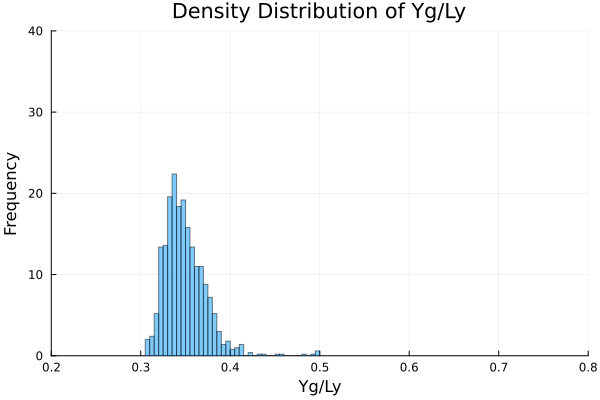
\includegraphics[width=\textwidth]{image/RaRtmap_hist/2023-11-15T07:34:00.555__chi1.265_Ay50_rho0.4_T0.43_dT0.04_Rd0.0_Rt0.375_Ra0.0_g0.0003999718779659611_run4.0e7_output.png}
      \subcaption{$\text{R}_\text{a}=0.0,\\\text{R}_\text{t}=0.375$}
      \label{}
    \end{minipage} &
    \begin{minipage}[t]{0.2\hsize}
      \centering
      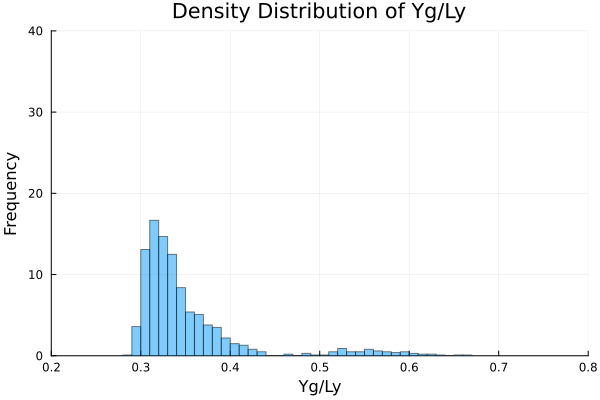
\includegraphics[width=\textwidth]{image/RaRtmap_hist/2023-11-15T08:24:37.362__chi1.265_Ay50_rho0.4_T0.43_dT0.04_Rd0.0_Rt0.375_Ra0.4693845_g0.0003999718779659611_run4.0e7_output.png}
      \subcaption{$\text{R}_\text{a}=0.469,\\\text{R}_\text{t}=0.375$}
      \label{}
    \end{minipage} &
    \begin{minipage}[t]{0.2\hsize}
      \centering
      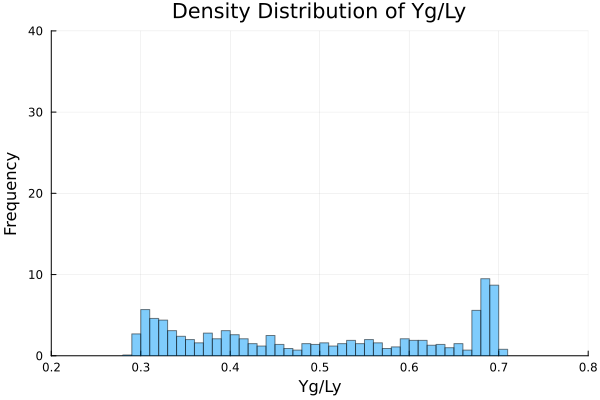
\includegraphics[width=\textwidth]{image/RaRtmap_hist/2023-11-15T09:16:40.082__chi1.265_Ay50_rho0.4_T0.43_dT0.04_Rd0.0_Rt0.375_Ra0.938769_g0.0003999718779659611_run4.0e7_output.png}
      \subcaption{$\text{R}_\text{a}=0.938,\\\text{R}_\text{t}=0.375$}
      \label{}
    \end{minipage} &
    \begin{minipage}[t]{0.2\hsize}
      \centering
      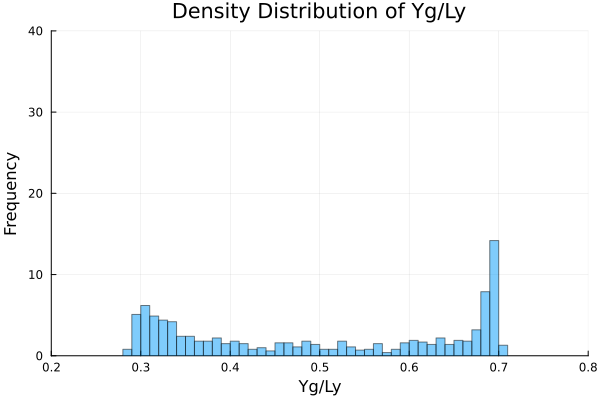
\includegraphics[width=\textwidth]{image/RaRtmap_hist/2023-11-15T10:07:20.945__chi1.265_Ay50_rho0.4_T0.43_dT0.04_Rd0.0_Rt0.375_Ra1.4081535_g0.0003999718779659611_run4.0e7_output.png}
      \subcaption{$\text{R}_\text{a}=1.408,\\\text{R}_\text{t}=0.375$}
      \label{}
    \end{minipage} &
    \begin{minipage}[t]{0.2\hsize}
      \centering
      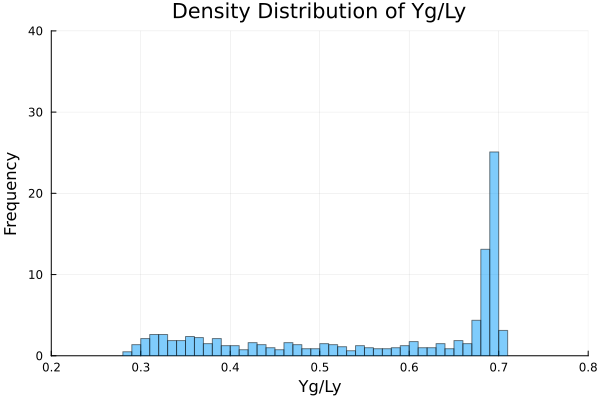
\includegraphics[width=\textwidth]{image/RaRtmap_hist/2023-11-15T10:59:30.665__chi1.265_Ay50_rho0.4_T0.43_dT0.04_Rd0.0_Rt0.375_Ra1.877538_g0.0003999718779659611_run4.0e7_output.png}
      \subcaption{$\text{R}_\text{a}=1.877,\\\text{R}_\text{t}=0.375$}
      \label{}
    \end{minipage} \\
    \begin{minipage}[t]{0.2\hsize}
      \centering
      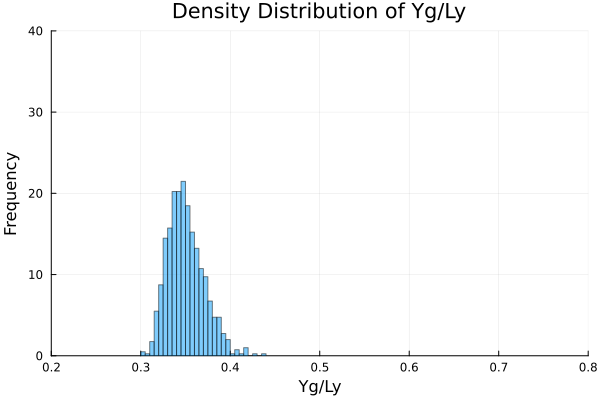
\includegraphics[width=\textwidth]{image/RaRtmap_hist/2023-11-15T11:53:37.697__chi1.265_Ay50_rho0.4_T0.43_dT0.04_Rd0.0_Rt0.5_Ra0.0_g0.0003999718779659611_run4.0e7_output.png}
      \subcaption{$\text{R}_\text{a}=0.0,\\\text{R}_\text{t}=0.500$}
      \label{}
    \end{minipage} &
    \begin{minipage}[t]{0.2\hsize}
      \centering
      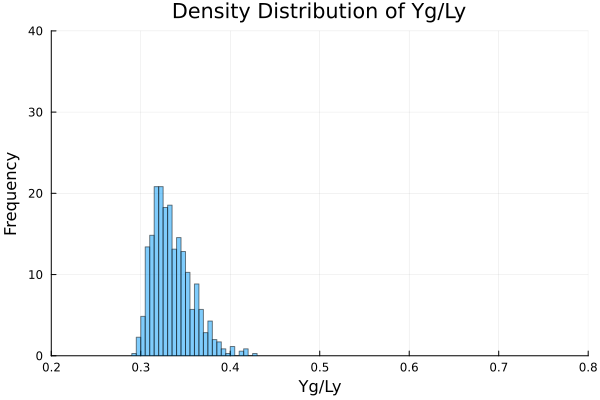
\includegraphics[width=\textwidth]{image/RaRtmap_hist/2023-11-15T12:45:26.303__chi1.265_Ay50_rho0.4_T0.43_dT0.04_Rd0.0_Rt0.5_Ra0.4693845_g0.0003999718779659611_run4.0e7_output.png}
      \subcaption{$\text{R}_\text{a}=0.469,\\\text{R}_\text{t}=0.500$}
      \label{fig:RaRtmap_hist_Ra0.469_Rt0.500}
    \end{minipage} &
    \begin{minipage}[t]{0.2\hsize}
      \centering
      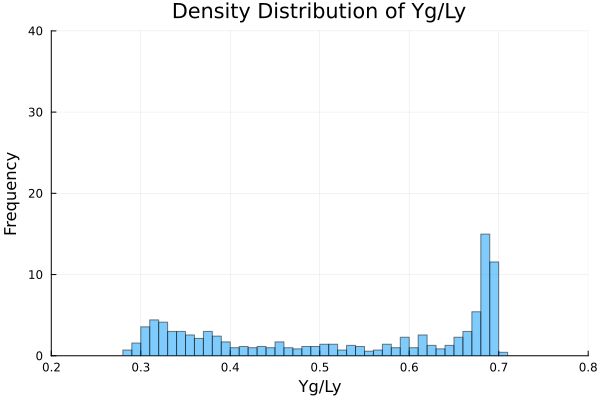
\includegraphics[width=\textwidth]{image/RaRtmap_hist/2023-11-15T13:37:58.058__chi1.265_Ay50_rho0.4_T0.43_dT0.04_Rd0.0_Rt0.5_Ra0.938769_g0.0003999718779659611_run4.0e7_output.png}
      \subcaption{$\text{R}_\text{a}=0.938,\\\text{R}_\text{t}=0.500$}
      \label{fig:RaRtmap_hist_Ra0.938_Rt0.500}
    \end{minipage} &
    \begin{minipage}[t]{0.2\hsize}
      \centering
      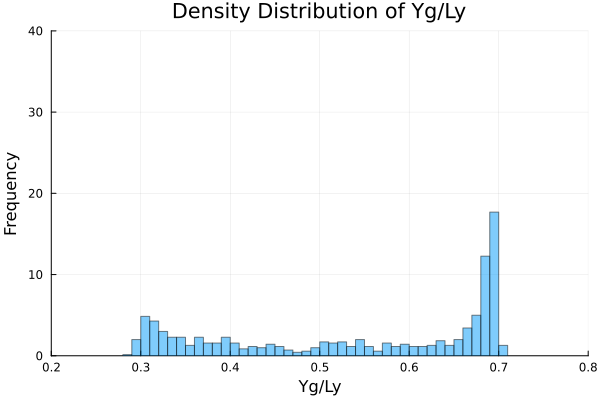
\includegraphics[width=\textwidth]{image/RaRtmap_hist/2023-11-15T14:30:22.529__chi1.265_Ay50_rho0.4_T0.43_dT0.04_Rd0.0_Rt0.5_Ra1.4081535_g0.0003999718779659611_run4.0e7_output.png}
      \subcaption{$\text{R}_\text{a}=1.408,\\\text{R}_\text{t}=0.500$}
      \label{}
    \end{minipage} &
    \begin{minipage}[t]{0.2\hsize}
      \centering
      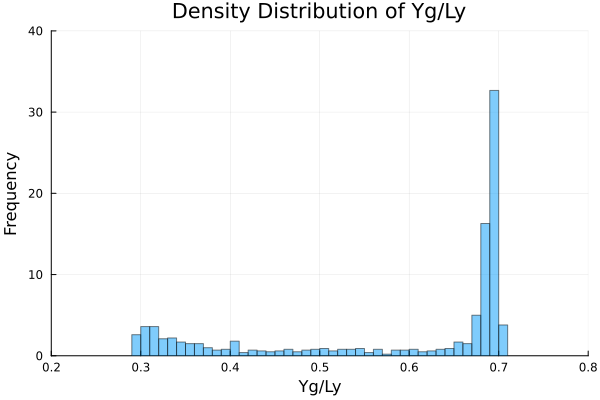
\includegraphics[width=\textwidth]{image/RaRtmap_hist/2023-11-15T15:21:59.073__chi1.265_Ay50_rho0.4_T0.43_dT0.04_Rd0.0_Rt0.5_Ra1.877538_g0.0003999718779659611_run4.0e7_output.png}
      \subcaption{$\text{R}_\text{a}=1.877,\\\text{R}_\text{t}=0.500$}
      \label{}
    \end{minipage} 
  \end{tabular}
  \caption{$t_i = 0, t_f = 2.0 \times 10^5, \dd t \sqrt{\varepsilon / m \sigma^2}= 0.005, t \sqrt{\varepsilon / m \sigma^2} = 200 ごとにY_g をプロットしたもののヒストグラム. ビン数は共通で50本.$}
  \label{}
\end{figure}


\subsection{重力を先にかけて, 熱流を後からかける}

\begin{figure}[H]
  \begin{tabular}{ccccc}
    \begin{minipage}[t]{0.2\hsize}
      \centering
      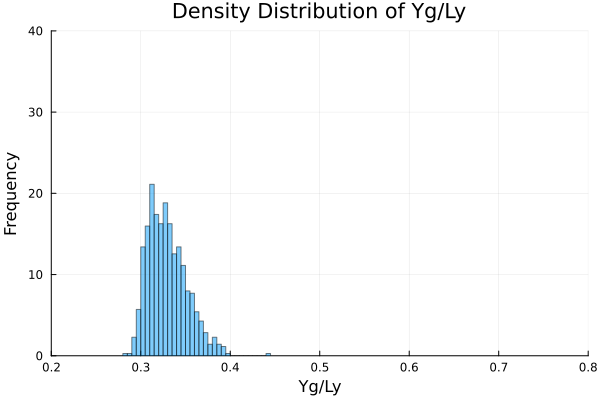
\includegraphics[width=\textwidth]{image/RaRtmap_drop_hist/2023-12-21T10:44:56.628_RaRtmap_chi1.265_Ay50_rho0.4_T0.43_dT0.04_Rd0.0_Rt0.0_Ra0.0_g0.0003999718779659611_run4.0e7.png}
      \subcaption{$\text{R}_\text{a}=0.0,\text{R}_\text{t}=0.0$}
      \label{fig:RaRtmap_drop_hist_Ra0.0_Rt0.0}
    \end{minipage} &
    \begin{minipage}[t]{0.2\hsize}
      \centering
      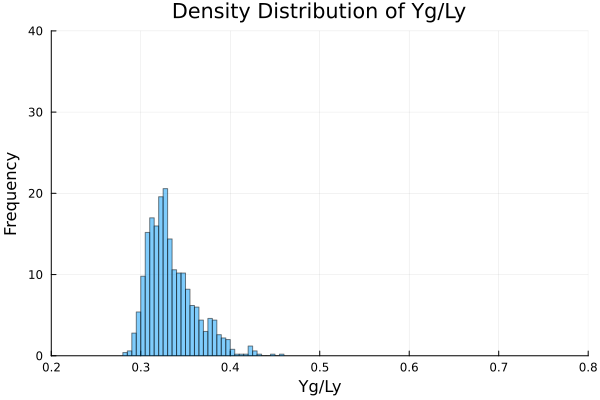
\includegraphics[width=\textwidth]{image/RaRtmap_drop_hist/2023-12-21T10:44:57.232_RaRtmap_chi1.265_Ay50_rho0.4_T0.43_dT0.04_Rd0.0_Rt0.0_Ra0.4693845_g0.0003999718779659611_run4.0e7.png}
      \subcaption{$\text{R}_\text{a}=0.469,\\\text{R}_\text{t}=0.0$}
      \label{}
    \end{minipage} &
    \begin{minipage}[t]{0.2\hsize}
      \centering
      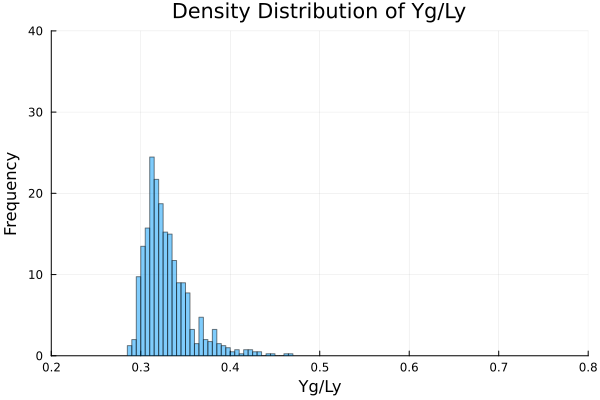
\includegraphics[width=\textwidth]{image/RaRtmap_drop_hist/2023-12-21T10:44:57.302_RaRtmap_chi1.265_Ay50_rho0.4_T0.43_dT0.04_Rd0.0_Rt0.0_Ra0.938769_g0.0003999718779659611_run4.0e7.png}
      \subcaption{$\text{R}_\text{a}=0.938,\\\text{R}_\text{t}=0.0$}
      \label{}
    \end{minipage} &
    \begin{minipage}[t]{0.2\hsize}
      \centering
      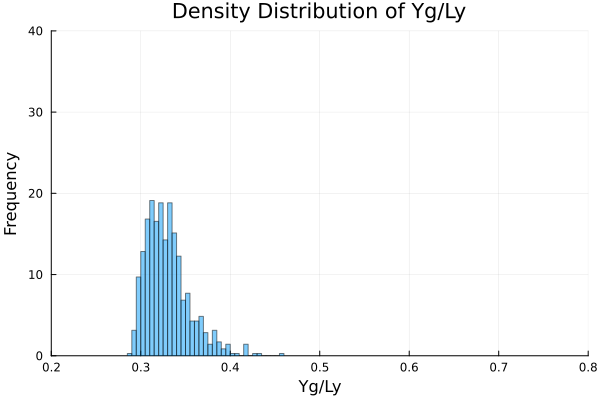
\includegraphics[width=\textwidth]{image/RaRtmap_drop_hist/2023-12-21T10:44:57.379_RaRtmap_chi1.265_Ay50_rho0.4_T0.43_dT0.04_Rd0.0_Rt0.0_Ra1.4081535_g0.0003999718779659611_run4.0e7.png}
      \subcaption{$\text{R}_\text{a}=1.408,\\\text{R}_\text{t}=0.0$}
      \label{}
    \end{minipage} &
    \begin{minipage}[t]{0.2\hsize}
      \centering
      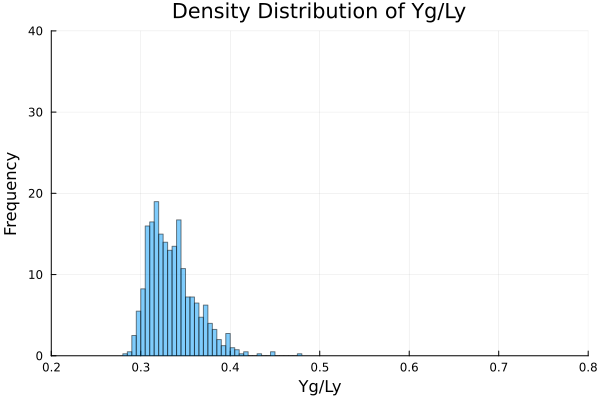
\includegraphics[width=\textwidth]{image/RaRtmap_drop_hist/2023-12-21T10:44:57.455_RaRtmap_chi1.265_Ay50_rho0.4_T0.43_dT0.04_Rd0.0_Rt0.0_Ra1.877538_g0.0003999718779659611_run4.0e7.png}
      \subcaption{$\text{R}_\text{a}=1.877,\\\text{R}_\text{t}=0.0$}
      \label{}
    \end{minipage} \\
    \begin{minipage}[t]{0.2\hsize}
      \centering
      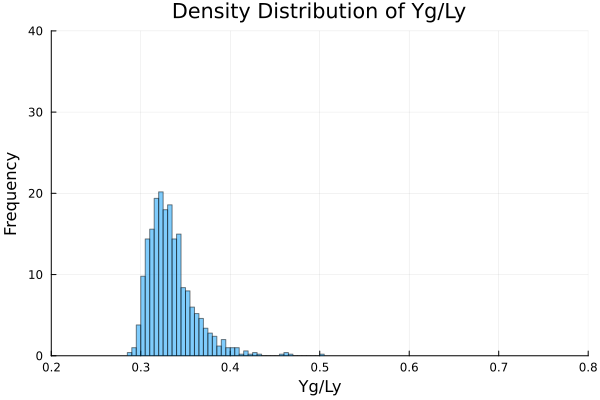
\includegraphics[width=\textwidth]{image/RaRtmap_drop_hist/2023-12-21T10:44:57.529_RaRtmap_chi1.265_Ay50_rho0.4_T0.43_dT0.04_Rd0.0_Rt0.125_Ra0.0_g0.0003999718779659611_run4.0e7.png}
      \subcaption{$\text{R}_\text{a}=0.0,\\\text{R}_\text{t}=0.125$}
      \label{}
    \end{minipage} &
    \begin{minipage}[t]{0.2\hsize}
      \centering
      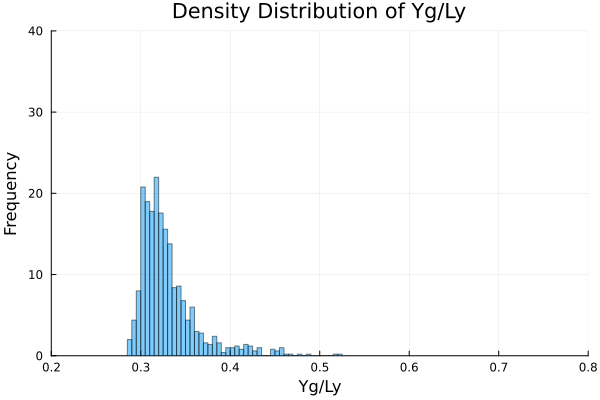
\includegraphics[width=\textwidth]{image/RaRtmap_drop_hist/2023-12-21T10:44:57.600_RaRtmap_chi1.265_Ay50_rho0.4_T0.43_dT0.04_Rd0.0_Rt0.125_Ra0.4693845_g0.0003999718779659611_run4.0e7.png}
      \subcaption{$\text{R}_\text{a}=0.469,\\\text{R}_\text{t}=0.125$}
      \label{}
    \end{minipage} &
    \begin{minipage}[t]{0.2\hsize}
      \centering
      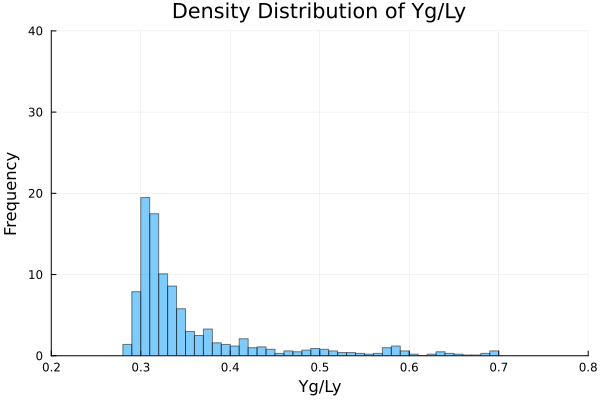
\includegraphics[width=\textwidth]{image/RaRtmap_drop_hist/2023-12-21T10:44:57.672_RaRtmap_chi1.265_Ay50_rho0.4_T0.43_dT0.04_Rd0.0_Rt0.125_Ra0.938769_g0.0003999718779659611_run4.0e7.png}
      \subcaption{$\text{R}_\text{a}=0.938,\\\text{R}_\text{t}=0.125$}
      \label{}
    \end{minipage} &
    \begin{minipage}[t]{0.2\hsize}
      \centering
      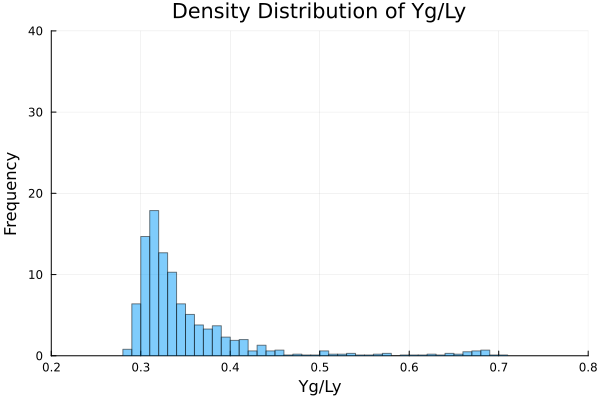
\includegraphics[width=\textwidth]{image/RaRtmap_drop_hist/2023-12-21T10:44:57.746_RaRtmap_chi1.265_Ay50_rho0.4_T0.43_dT0.04_Rd0.0_Rt0.125_Ra1.4081535_g0.0003999718779659611_run4.0e7.png}
      \subcaption{$\text{R}_\text{a}=1.408,\\\text{R}_\text{t}=0.125$}
      \label{}
    \end{minipage} &
    \begin{minipage}[t]{0.2\hsize}
      \centering
      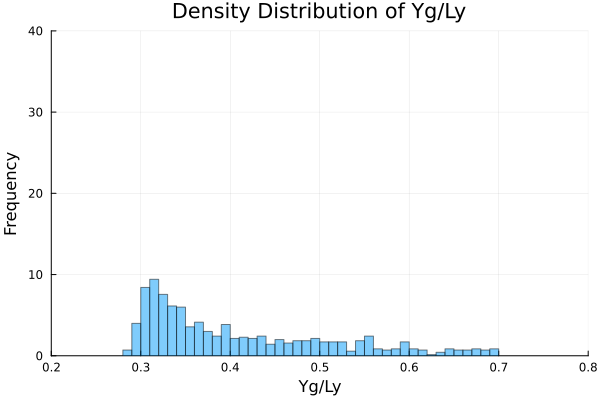
\includegraphics[width=\textwidth]{image/RaRtmap_drop_hist/2023-12-21T10:44:57.821_RaRtmap_chi1.265_Ay50_rho0.4_T0.43_dT0.04_Rd0.0_Rt0.125_Ra1.877538_g0.0003999718779659611_run4.0e7.png}
      \subcaption{$\text{R}_\text{a}=1.877,\\\text{R}_\text{t}=0.125$}
      \label{}
    \end{minipage} \\
    \begin{minipage}[t]{0.2\hsize}
      \centering
      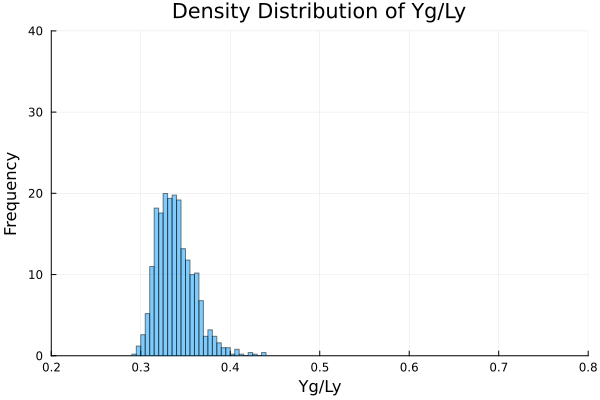
\includegraphics[width=\textwidth]{image/RaRtmap_drop_hist/2023-12-21T10:44:57.897_RaRtmap_chi1.265_Ay50_rho0.4_T0.43_dT0.04_Rd0.0_Rt0.25_Ra0.0_g0.0003999718779659611_run4.0e7.png}
      \subcaption{$\text{R}_\text{a}=0.0,\\\text{R}_\text{t}=0.250$}
      \label{}
    \end{minipage} &
    \begin{minipage}[t]{0.2\hsize}
      \centering
      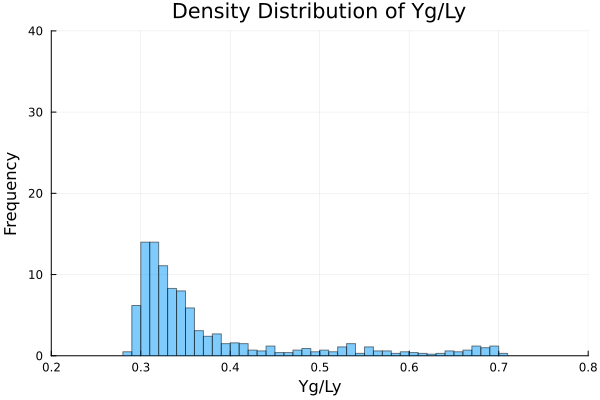
\includegraphics[width=\textwidth]{image/RaRtmap_drop_hist/2023-12-21T10:44:57.979_RaRtmap_chi1.265_Ay50_rho0.4_T0.43_dT0.04_Rd0.0_Rt0.25_Ra0.4693845_g0.0003999718779659611_run4.0e7.png}
      \subcaption{$\text{R}_\text{a}=0.469,\\\text{R}_\text{t}=0.250$}
      \label{}
    \end{minipage} &
    \begin{minipage}[t]{0.2\hsize}
      \centering
      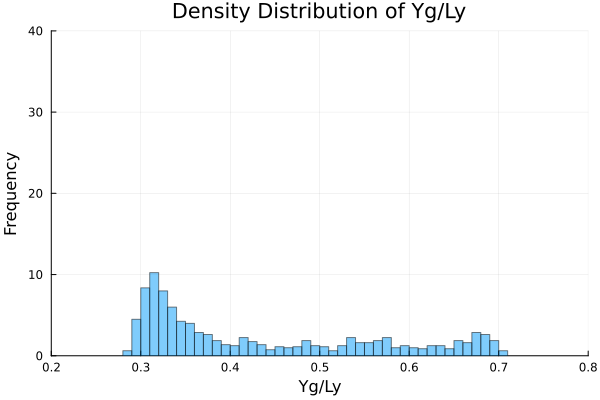
\includegraphics[width=\textwidth]{image/RaRtmap_drop_hist/2023-12-21T10:44:58.051_RaRtmap_chi1.265_Ay50_rho0.4_T0.43_dT0.04_Rd0.0_Rt0.25_Ra0.938769_g0.0003999718779659611_run4.0e7.png}
      \subcaption{$\text{R}_\text{a}=0.938,\\\text{R}_\text{t}=0.250$}
      \label{}
    \end{minipage} &
    \begin{minipage}[t]{0.2\hsize}
      \centering
      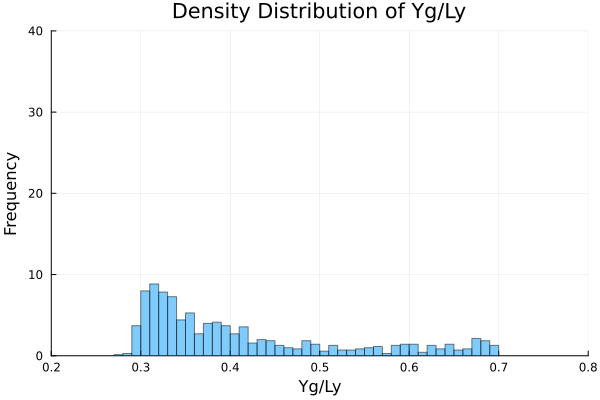
\includegraphics[width=\textwidth]{image/RaRtmap_drop_hist/2023-12-21T10:44:58.129_RaRtmap_chi1.265_Ay50_rho0.4_T0.43_dT0.04_Rd0.0_Rt0.25_Ra1.4081535_g0.0003999718779659611_run4.0e7.png}
      \subcaption{$\text{R}_\text{a}=1.408,\\\text{R}_\text{t}=0.250$}
      \label{}
    \end{minipage} &
    \begin{minipage}[t]{0.2\hsize}
      \centering
      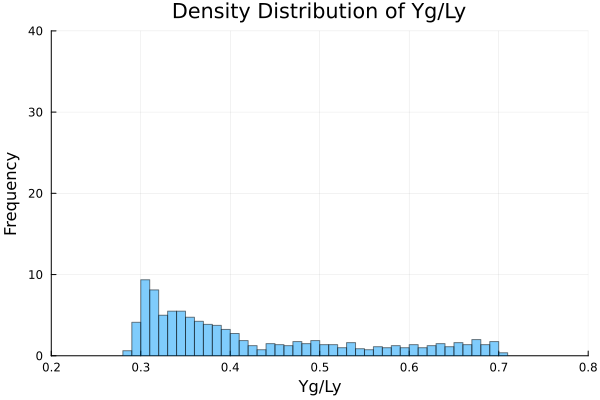
\includegraphics[width=\textwidth]{image/RaRtmap_drop_hist/2023-12-21T10:44:58.197_RaRtmap_chi1.265_Ay50_rho0.4_T0.43_dT0.04_Rd0.0_Rt0.25_Ra1.877538_g0.0003999718779659611_run4.0e7.png}
      \subcaption{$\text{R}_\text{a}=1.877,\\\text{R}_\text{t}=0.250$}
      \label{}
    \end{minipage} \\
    \begin{minipage}[t]{0.2\hsize}
      \centering
      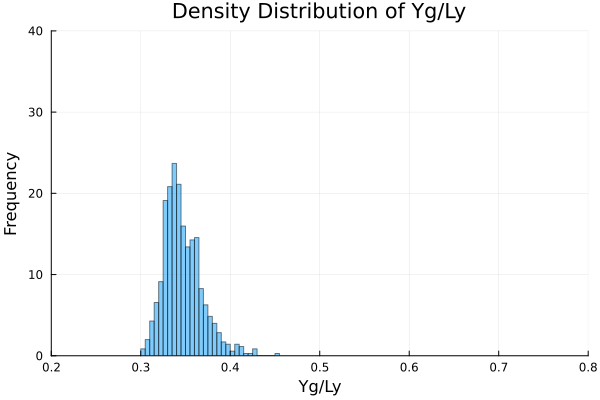
\includegraphics[width=\textwidth]{image/RaRtmap_drop_hist/2023-12-21T10:44:58.258_RaRtmap_chi1.265_Ay50_rho0.4_T0.43_dT0.04_Rd0.0_Rt0.375_Ra0.0_g0.0003999718779659611_run4.0e7.png}
      \subcaption{$\text{R}_\text{a}=0.0,\\\text{R}_\text{t}=0.375$}
      \label{}
    \end{minipage} &
    \begin{minipage}[t]{0.2\hsize}
      \centering
      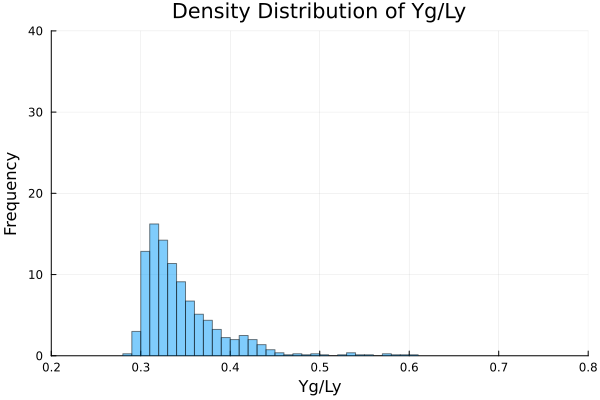
\includegraphics[width=\textwidth]{image/RaRtmap_drop_hist/2023-12-21T10:44:58.322_RaRtmap_chi1.265_Ay50_rho0.4_T0.43_dT0.04_Rd0.0_Rt0.375_Ra0.4693845_g0.0003999718779659611_run4.0e7.png}
      \subcaption{$\text{R}_\text{a}=0.469,\\\text{R}_\text{t}=0.375$}
      \label{}
    \end{minipage} &
    \begin{minipage}[t]{0.2\hsize}
      \centering
      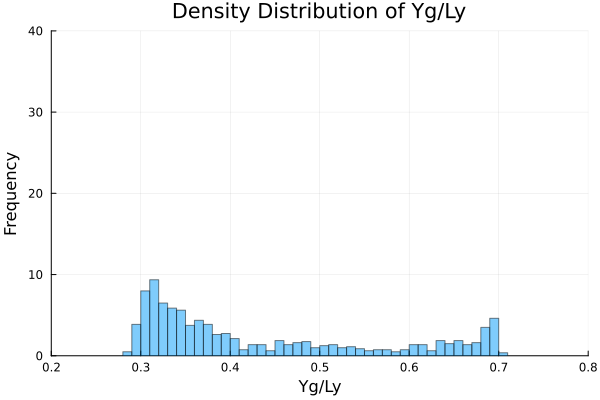
\includegraphics[width=\textwidth]{image/RaRtmap_drop_hist/2023-12-21T10:44:58.387_RaRtmap_chi1.265_Ay50_rho0.4_T0.43_dT0.04_Rd0.0_Rt0.375_Ra0.938769_g0.0003999718779659611_run4.0e7.png}
      \subcaption{$\text{R}_\text{a}=0.938,\\\text{R}_\text{t}=0.375$}
      \label{}
    \end{minipage} &
    \begin{minipage}[t]{0.2\hsize}
      \centering
      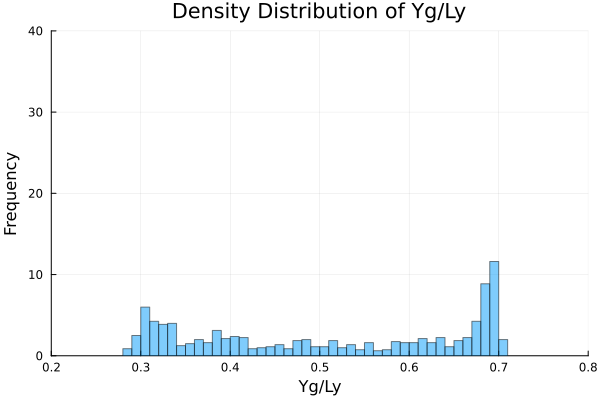
\includegraphics[width=\textwidth]{image/RaRtmap_drop_hist/2023-12-21T10:44:58.471_RaRtmap_chi1.265_Ay50_rho0.4_T0.43_dT0.04_Rd0.0_Rt0.375_Ra1.4081535_g0.0003999718779659611_run4.0e7.png}
      \subcaption{$\text{R}_\text{a}=1.408,\\\text{R}_\text{t}=0.375$}
      \label{}
    \end{minipage} &
    \begin{minipage}[t]{0.2\hsize}
      \centering
      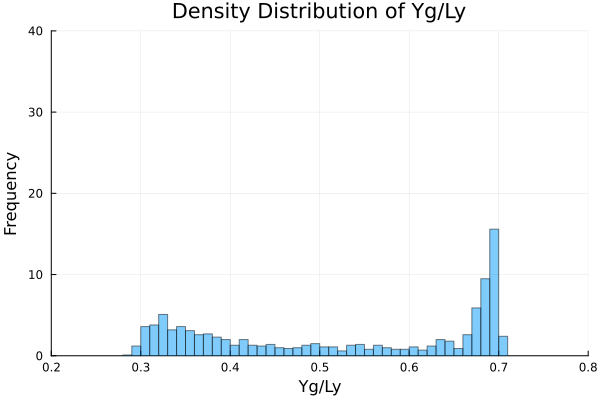
\includegraphics[width=\textwidth]{image/RaRtmap_drop_hist/2023-12-21T10:44:58.541_RaRtmap_chi1.265_Ay50_rho0.4_T0.43_dT0.04_Rd0.0_Rt0.375_Ra1.877538_g0.0003999718779659611_run4.0e7.png}
      \subcaption{$\text{R}_\text{a}=1.877,\\\text{R}_\text{t}=0.375$}
      \label{}
    \end{minipage} \\
    \begin{minipage}[t]{0.2\hsize}
      \centering
      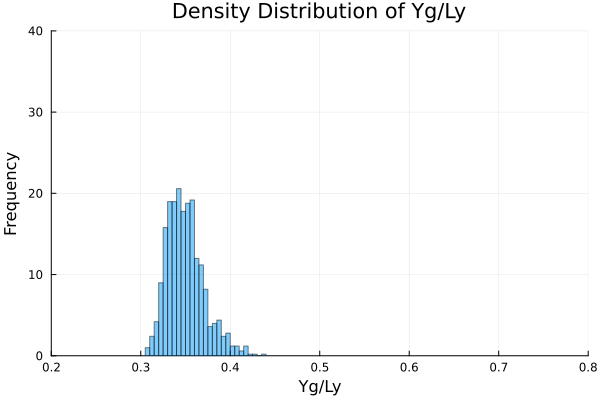
\includegraphics[width=\textwidth]{image/RaRtmap_drop_hist/2023-12-21T10:44:58.621_RaRtmap_chi1.265_Ay50_rho0.4_T0.43_dT0.04_Rd0.0_Rt0.5_Ra0.0_g0.0003999718779659611_run4.0e7.png}
      \subcaption{$\text{R}_\text{a}=0.0,\\\text{R}_\text{t}=0.500$}
      \label{}
    \end{minipage} &
    \begin{minipage}[t]{0.2\hsize}
      \centering
      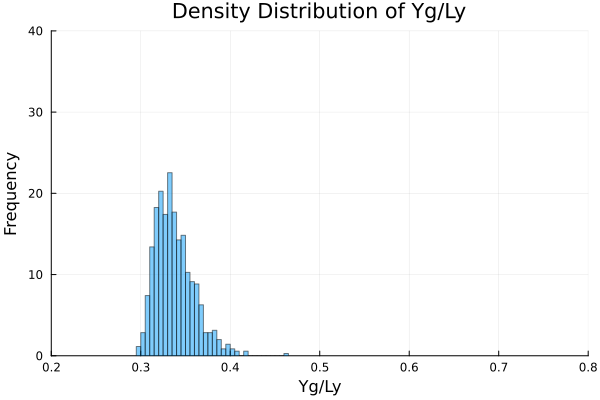
\includegraphics[width=\textwidth]{image/RaRtmap_drop_hist/2023-12-21T10:44:58.706_RaRtmap_chi1.265_Ay50_rho0.4_T0.43_dT0.04_Rd0.0_Rt0.5_Ra0.4693845_g0.0003999718779659611_run4.0e7.png}
      \subcaption{$\text{R}_\text{a}=0.469,\\\text{R}_\text{t}=0.500$}
      \label{fig:RaRtmap_drop_hist_Ra0.469_Rt0.500}
    \end{minipage} &
    \begin{minipage}[t]{0.2\hsize}
      \centering
      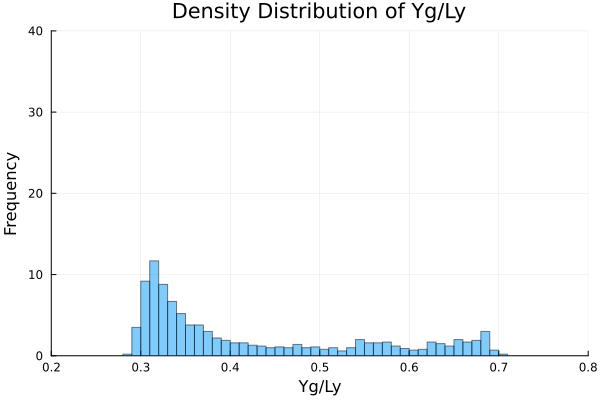
\includegraphics[width=\textwidth]{image/RaRtmap_drop_hist/2023-12-21T10:44:58.788_RaRtmap_chi1.265_Ay50_rho0.4_T0.43_dT0.04_Rd0.0_Rt0.5_Ra0.938769_g0.0003999718779659611_run4.0e7.png}
      \subcaption{$\text{R}_\text{a}=0.938,\\\text{R}_\text{t}=0.500$}
      \label{fig:RaRtmap_drop_hist_Ra0.938_Rt0.500}
    \end{minipage} &
    \begin{minipage}[t]{0.2\hsize}
      \centering
      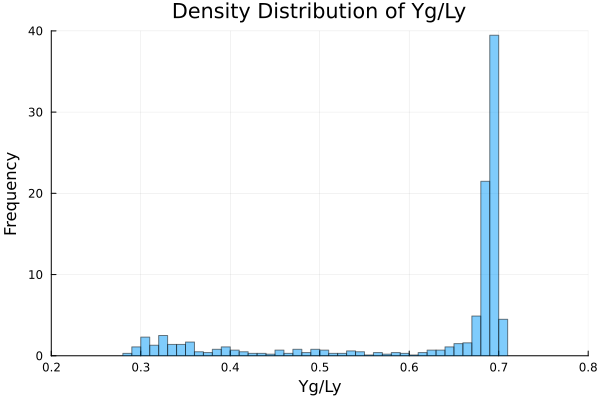
\includegraphics[width=\textwidth]{image/RaRtmap_drop_hist/2023-12-21T10:44:58.872_RaRtmap_chi1.265_Ay50_rho0.4_T0.43_dT0.04_Rd0.0_Rt0.5_Ra1.4081535_g0.0003999718779659611_run4.0e7.png}
      \subcaption{$\text{R}_\text{a}=1.408,\\\text{R}_\text{t}=0.500$}
      \label{}
    \end{minipage} &
    \begin{minipage}[t]{0.2\hsize}
      \centering
      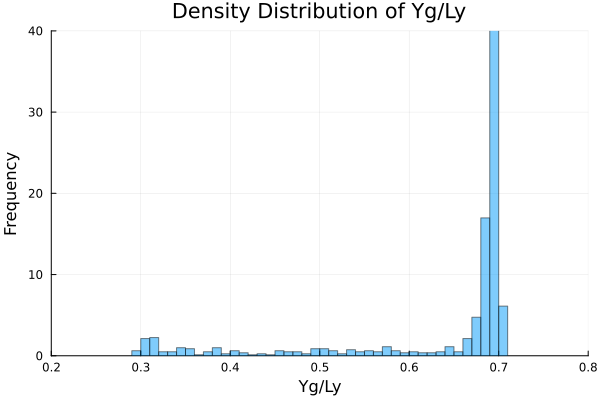
\includegraphics[width=\textwidth]{image/RaRtmap_drop_hist/2023-12-21T10:44:58.955_RaRtmap_chi1.265_Ay50_rho0.4_T0.43_dT0.04_Rd0.0_Rt0.5_Ra1.877538_g0.0003999718779659611_run4.0e7.png}
      \subcaption{$\text{R}_\text{a}=1.877,\\\text{R}_\text{t}=0.500$}
      \label{}
    \end{minipage} 
  \end{tabular}
  \caption{$t_i = 2.4 \times 10^5, t_f = 4.0 \times 10^5, \dd t \sqrt{\varepsilon / m \sigma^2}= 0.005, t \sqrt{\varepsilon / m \sigma^2} = 200 ごとにプロット.$}
  \label{fig:RaRtmap_drop_hist}
\end{figure}


\subsection{重力のみをかける}

\begin{figure}[H]
  \begin{tabular}{ccccc}
    \begin{minipage}[t]{0.2\hsize}
      \centering
      \includegraphics[width=\textwidth]{image/dT0_hist/2024-01-15T14:30:46.366_mapg0_chi0_Ay50_rho0.4_T0.43_dT0.0_Rd0.0_Rt0.0_Ra0.0_g0.0003999718779659611_run4.0e7.png}
      \subcaption{$\text{R}_\text{a}=0.0,\\\text{R}_\text{t}=0.0$}
      \label{fig:dT0_hist_Ra0.0_Rt0.0}
    \end{minipage} &
    \begin{minipage}[t]{0.2\hsize}
      \centering
      \includegraphics[width=\textwidth]{image/dT0_hist/2024-01-15T14:30:46.901_mapg0_chi0_Ay50_rho0.4_T0.43_dT0.0_Rd0.0_Rt0.0_Ra0.4693845_g0.0003999718779659611_run4.0e7.png}
      \subcaption{$\text{R}_\text{a}=0.469,\\\text{R}_\text{t}=0.0$}
      \label{}
    \end{minipage} &
    \begin{minipage}[t]{0.2\hsize}
      \centering
      \includegraphics[width=\textwidth]{image/dT0_hist/2024-01-15T14:30:46.968_mapg0_chi0_Ay50_rho0.4_T0.43_dT0.0_Rd0.0_Rt0.0_Ra0.938769_g0.0003999718779659611_run4.0e7.png}
      \subcaption{$\text{R}_\text{a}=0.938,\\\text{R}_\text{t}=0.0$}
      \label{}
    \end{minipage} &
    \begin{minipage}[t]{0.2\hsize}
      \centering
      \includegraphics[width=\textwidth]{image/dT0_hist/2024-01-15T14:30:47.037_mapg0_chi0_Ay50_rho0.4_T0.43_dT0.0_Rd0.0_Rt0.0_Ra1.4081535_g0.0003999718779659611_run4.0e7.png}
      \subcaption{$\text{R}_\text{a}=1.408,\\\text{R}_\text{t}=0.0$}
      \label{}
    \end{minipage} &
    \begin{minipage}[t]{0.2\hsize}
      \centering
      \includegraphics[width=\textwidth]{image/dT0_hist/2024-01-15T14:30:47.119_mapg0_chi0_Ay50_rho0.4_T0.43_dT0.0_Rd0.0_Rt0.0_Ra1.877538_g0.0003999718779659611_run4.0e7.png}
      \subcaption{$\text{R}_\text{a}=1.877,\\\text{R}_\text{t}=0.0$}
      \label{}
    \end{minipage} \\
    \begin{minipage}[t]{0.2\hsize}
      \centering
      \includegraphics[width=\textwidth]{image/dT0_hist/2024-01-15T14:30:47.186_mapg0_chi0_Ay50_rho0.4_T0.43_dT0.0_Rd0.0_Rt0.125_Ra0.0_g0.0003999718779659611_run4.0e7.png}
      \subcaption{$\text{R}_\text{a}=0.0,\\\text{R}_\text{t}=0.125$}
      \label{}
    \end{minipage} &
    \begin{minipage}[t]{0.2\hsize}
      \centering
      \includegraphics[width=\textwidth]{image/dT0_hist/2024-01-15T14:30:47.255_mapg0_chi0_Ay50_rho0.4_T0.43_dT0.0_Rd0.0_Rt0.125_Ra0.4693845_g0.0003999718779659611_run4.0e7.png}
      \subcaption{$\text{R}_\text{a}=0.469,\\\text{R}_\text{t}=0.125$}
      \label{}
    \end{minipage} &
    \begin{minipage}[t]{0.2\hsize}
      \centering
      \includegraphics[width=\textwidth]{image/dT0_hist/2024-01-15T14:30:47.323_mapg0_chi0_Ay50_rho0.4_T0.43_dT0.0_Rd0.0_Rt0.125_Ra0.938769_g0.0003999718779659611_run4.0e7.png}
      \subcaption{$\text{R}_\text{a}=0.938,\\\text{R}_\text{t}=0.125$}
      \label{}
    \end{minipage} &
    \begin{minipage}[t]{0.2\hsize}
      \centering
      \includegraphics[width=\textwidth]{image/dT0_hist/2024-01-15T14:30:47.390_mapg0_chi0_Ay50_rho0.4_T0.43_dT0.0_Rd0.0_Rt0.125_Ra1.4081535_g0.0003999718779659611_run4.0e7.png}
      \subcaption{$\text{R}_\text{a}=1.408,\\\text{R}_\text{t}=0.125$}
      \label{}
    \end{minipage} &
    \begin{minipage}[t]{0.2\hsize}
      \centering
      \includegraphics[width=\textwidth]{image/dT0_hist/2024-01-15T14:30:47.459_mapg0_chi0_Ay50_rho0.4_T0.43_dT0.0_Rd0.0_Rt0.125_Ra1.877538_g0.0003999718779659611_run4.0e7.png}
      \subcaption{$\text{R}_\text{a}=1.877,\\\text{R}_\text{t}=0.125$}
      \label{}
    \end{minipage} \\
    \begin{minipage}[t]{0.2\hsize}
      \centering
      \includegraphics[width=\textwidth]{image/dT0_hist/2024-01-15T14:30:47.525_mapg0_chi0_Ay50_rho0.4_T0.43_dT0.0_Rd0.0_Rt0.25_Ra0.0_g0.0003999718779659611_run4.0e7.png}
      \subcaption{$\text{R}_\text{a}=0.0,\\\text{R}_\text{t}=0.250$}
      \label{}
    \end{minipage} &
    \begin{minipage}[t]{0.2\hsize}
      \centering
      \includegraphics[width=\textwidth]{image/dT0_hist/2024-01-15T14:30:47.592_mapg0_chi0_Ay50_rho0.4_T0.43_dT0.0_Rd0.0_Rt0.25_Ra0.4693845_g0.0003999718779659611_run4.0e7.png}
      \subcaption{$\text{R}_\text{a}=0.469,\\\text{R}_\text{t}=0.250$}
      \label{}
    \end{minipage} &
    \begin{minipage}[t]{0.2\hsize}
      \centering
      \includegraphics[width=\textwidth]{image/dT0_hist/2024-01-15T14:30:47.659_mapg0_chi0_Ay50_rho0.4_T0.43_dT0.0_Rd0.0_Rt0.25_Ra0.938769_g0.0003999718779659611_run4.0e7.png}
      \subcaption{$\text{R}_\text{a}=0.938,\\\text{R}_\text{t}=0.250$}
      \label{}
    \end{minipage} &
    \begin{minipage}[t]{0.2\hsize}
      \centering
      \includegraphics[width=\textwidth]{image/dT0_hist/2024-01-15T14:30:47.726_mapg0_chi0_Ay50_rho0.4_T0.43_dT0.0_Rd0.0_Rt0.25_Ra1.4081535_g0.0003999718779659611_run4.0e7.png}
      \subcaption{$\text{R}_\text{a}=1.408,\\\text{R}_\text{t}=0.250$}
      \label{}
    \end{minipage} &
    \begin{minipage}[t]{0.2\hsize}
      \centering
      \includegraphics[width=\textwidth]{image/dT0_hist/2024-01-15T14:30:47.794_mapg0_chi0_Ay50_rho0.4_T0.43_dT0.0_Rd0.0_Rt0.25_Ra1.877538_g0.0003999718779659611_run4.0e7.png}
      \subcaption{$\text{R}_\text{a}=1.877,\\\text{R}_\text{t}=0.250$}
      \label{}
    \end{minipage} \\
    \begin{minipage}[t]{0.2\hsize}
      \centering
      \includegraphics[width=\textwidth]{image/dT0_hist/2024-01-15T14:30:47.876_mapg0_chi0_Ay50_rho0.4_T0.43_dT0.0_Rd0.0_Rt0.375_Ra0.0_g0.0003999718779659611_run4.0e7.png}
      \subcaption{$\text{R}_\text{a}=0.0,\\\text{R}_\text{t}=0.375$}
      \label{}
    \end{minipage} &
    \begin{minipage}[t]{0.2\hsize}
      \centering
      \includegraphics[width=\textwidth]{image/dT0_hist/2024-01-15T14:30:47.945_mapg0_chi0_Ay50_rho0.4_T0.43_dT0.0_Rd0.0_Rt0.375_Ra0.4693845_g0.0003999718779659611_run4.0e7.png}
      \subcaption{$\text{R}_\text{a}=0.469,\\\text{R}_\text{t}=0.375$}
      \label{}
    \end{minipage} &
    \begin{minipage}[t]{0.2\hsize}
      \centering
      \includegraphics[width=\textwidth]{image/dT0_hist/2024-01-15T14:30:48.012_mapg0_chi0_Ay50_rho0.4_T0.43_dT0.0_Rd0.0_Rt0.375_Ra0.938769_g0.0003999718779659611_run4.0e7.png}
      \subcaption{$\text{R}_\text{a}=0.938,\\\text{R}_\text{t}=0.375$}
      \label{}
    \end{minipage} &
    \begin{minipage}[t]{0.2\hsize}
      \centering
      \includegraphics[width=\textwidth]{image/dT0_hist/2024-01-15T14:30:48.081_mapg0_chi0_Ay50_rho0.4_T0.43_dT0.0_Rd0.0_Rt0.375_Ra1.4081535_g0.0003999718779659611_run4.0e7.png}
      \subcaption{$\text{R}_\text{a}=1.408,\\\text{R}_\text{t}=0.375$}
      \label{}
    \end{minipage} &
    \begin{minipage}[t]{0.2\hsize}
      \centering
      \includegraphics[width=\textwidth]{image/dT0_hist/2024-01-15T14:30:48.147_mapg0_chi0_Ay50_rho0.4_T0.43_dT0.0_Rd0.0_Rt0.375_Ra1.877538_g0.0003999718779659611_run4.0e7.png}
      \subcaption{$\text{R}_\text{a}=1.877,\\\text{R}_\text{t}=0.375$}
      \label{}
    \end{minipage} \\
    \begin{minipage}[t]{0.2\hsize}
      \centering
      \includegraphics[width=\textwidth]{image/dT0_hist/2024-01-15T14:30:48.227_mapg0_chi0_Ay50_rho0.4_T0.43_dT0.0_Rd0.0_Rt0.5_Ra0.0_g0.0003999718779659611_run4.0e7.png}
      \subcaption{$\text{R}_\text{a}=0.0,\\\text{R}_\text{t}=0.500$}
      \label{}
    \end{minipage} &
    \begin{minipage}[t]{0.2\hsize}
      \centering
      \includegraphics[width=\textwidth]{image/dT0_hist/2024-01-15T14:30:48.295_mapg0_chi0_Ay50_rho0.4_T0.43_dT0.0_Rd0.0_Rt0.5_Ra0.4693845_g0.0003999718779659611_run4.0e7.png}
      \subcaption{$\text{R}_\text{a}=0.469,\\\text{R}_\text{t}=0.500$}
      \label{fig:dT0_hist_Ra0.469_Rt0.500}
    \end{minipage} &
    \begin{minipage}[t]{0.2\hsize}
      \centering
      \includegraphics[width=\textwidth]{image/dT0_hist/2024-01-15T14:30:48.365_mapg0_chi0_Ay50_rho0.4_T0.43_dT0.0_Rd0.0_Rt0.5_Ra0.938769_g0.0003999718779659611_run4.0e7.png}
      \subcaption{$\text{R}_\text{a}=0.938,\\\text{R}_\text{t}=0.500$}
      \label{fig:dT0_hist_Ra0.938_Rt0.500}
    \end{minipage} &
    \begin{minipage}[t]{0.2\hsize}
      \centering
      \includegraphics[width=\textwidth]{image/dT0_hist/2024-01-15T14:30:48.432_mapg0_chi0_Ay50_rho0.4_T0.43_dT0.0_Rd0.0_Rt0.5_Ra1.4081535_g0.0003999718779659611_run4.0e7.png}
      \subcaption{$\text{R}_\text{a}=1.408,\\\text{R}_\text{t}=0.500$}
      \label{}
    \end{minipage} &
    \begin{minipage}[t]{0.2\hsize}
      \centering
      \includegraphics[width=\textwidth]{image/dT0_hist/2024-01-15T14:30:48.499_mapg0_chi0_Ay50_rho0.4_T0.43_dT0.0_Rd0.0_Rt0.5_Ra1.877538_g0.0003999718779659611_run4.0e7.png}
      \subcaption{$\text{R}_\text{a}=1.877,\\\text{R}_\text{t}=0.500$}
      \label{}
    \end{minipage} 
  \end{tabular}
  \caption{$t_i = 4.0 \times 10^4 , t_f = 2.0 \times 10^5, \dd t \sqrt{\varepsilon / m \sigma^2}= 0.005, t \sqrt{\varepsilon / m \sigma^2} = 200 ごとにプロット.$}
  \label{fig:dT0_hist}
\end{figure}


\subsection{熱流のみをかける}

\begin{figure}[H]
  \begin{tabular}{ccccc}
    \begin{minipage}[t]{0.2\hsize}
      \centering
      \includegraphics[width=\textwidth]{image/g0_hist/2024-01-15T14:07:33.905_mapg0_chiinf_Ay50_rho0.4_T0.43_dT0.04_Rd0.0_Rt0.0_Ra0.0_g0_run4.0e7.png}
      \subcaption{$\text{R}_\text{a}=0.0,\text{R}_\text{t}=0.0$} % あとで差し替え.
      \label{fig:g0_hist_Ra0.0_Rt0.0}
    \end{minipage} &
    \begin{minipage}[t]{0.2\hsize}
      \centering
      \includegraphics[width=\textwidth]{image/g0_hist/2024-01-15T14:07:34.556_mapg0_chiinf_Ay50_rho0.4_T0.43_dT0.04_Rd0.0_Rt0.0_Ra0.4693845_g0_run4.0e7.png}
      \subcaption{$\text{R}_\text{a}=0.469,\\\text{R}_\text{t}=0.0$}
      \label{}
    \end{minipage} &
    \begin{minipage}[t]{0.2\hsize}
      \centering
      \includegraphics[width=\textwidth]{image/g0_hist/2024-01-15T14:07:34.622_mapg0_chiinf_Ay50_rho0.4_T0.43_dT0.04_Rd0.0_Rt0.0_Ra0.938769_g0_run4.0e7.png}
      \subcaption{$\text{R}_\text{a}=0.938,\\\text{R}_\text{t}=0.0$}
      \label{}
    \end{minipage} &
    \begin{minipage}[t]{0.2\hsize}
      \centering
      \includegraphics[width=\textwidth]{image/g0_hist/2024-01-15T14:07:34.689_mapg0_chiinf_Ay50_rho0.4_T0.43_dT0.04_Rd0.0_Rt0.0_Ra1.4081535_g0_run4.0e7.png}
      \subcaption{$\text{R}_\text{a}=1.408,\\\text{R}_\text{t}=0.0$}
      \label{}
    \end{minipage} &
    \begin{minipage}[t]{0.2\hsize}
      \centering
      \includegraphics[width=\textwidth]{image/g0_hist/2024-01-15T14:07:34.770_mapg0_chiinf_Ay50_rho0.4_T0.43_dT0.04_Rd0.0_Rt0.0_Ra1.877538_g0_run4.0e7.png}
      \subcaption{$\text{R}_\text{a}=1.877,\\\text{R}_\text{t}=0.0$}
      \label{}
    \end{minipage} \\
    \begin{minipage}[t]{0.2\hsize}
      \centering
      \includegraphics[width=\textwidth]{image/g0_hist/2024-01-15T14:07:34.852_mapg0_chiinf_Ay50_rho0.4_T0.43_dT0.04_Rd0.0_Rt0.125_Ra0.0_g0_run4.0e7.png}
      \subcaption{$\text{R}_\text{a}=0.0,\\\text{R}_\text{t}=0.125$}
      \label{}
    \end{minipage} &
    \begin{minipage}[t]{0.2\hsize}
      \centering
      \includegraphics[width=\textwidth]{image/g0_hist/2024-01-15T14:07:34.918_mapg0_chiinf_Ay50_rho0.4_T0.43_dT0.04_Rd0.0_Rt0.125_Ra0.4693845_g0_run4.0e7.png}
      \subcaption{$\text{R}_\text{a}=0.469,\\\text{R}_\text{t}=0.125$}
      \label{}
    \end{minipage} &
    \begin{minipage}[t]{0.2\hsize}
      \centering
      \includegraphics[width=\textwidth]{image/g0_hist/2024-01-15T14:07:34.988_mapg0_chiinf_Ay50_rho0.4_T0.43_dT0.04_Rd0.0_Rt0.125_Ra0.938769_g0_run4.0e7.png}
      \subcaption{$\text{R}_\text{a}=0.938,\\\text{R}_\text{t}=0.125$}
      \label{}
    \end{minipage} &
    \begin{minipage}[t]{0.2\hsize}
      \centering
      \includegraphics[width=\textwidth]{image/g0_hist/2024-01-15T14:07:35.058_mapg0_chiinf_Ay50_rho0.4_T0.43_dT0.04_Rd0.0_Rt0.125_Ra1.4081535_g0_run4.0e7.png}
      \subcaption{$\text{R}_\text{a}=1.408,\\\text{R}_\text{t}=0.125$}
      \label{}
    \end{minipage} &
    \begin{minipage}[t]{0.2\hsize}
      \centering
      \includegraphics[width=\textwidth]{image/g0_hist/2024-01-15T14:07:35.126_mapg0_chiinf_Ay50_rho0.4_T0.43_dT0.04_Rd0.0_Rt0.125_Ra1.877538_g0_run4.0e7.png}
      \subcaption{$\text{R}_\text{a}=1.877,\\\text{R}_\text{t}=0.125$}
      \label{}
    \end{minipage} \\
    \begin{minipage}[t]{0.2\hsize}
      \centering
      \includegraphics[width=\textwidth]{image/g0_hist/2024-01-15T14:07:35.195_mapg0_chiinf_Ay50_rho0.4_T0.43_dT0.04_Rd0.0_Rt0.25_Ra0.0_g0_run4.0e7.png}
      \subcaption{$\text{R}_\text{a}=0.0,\\\text{R}_\text{t}=0.250$}
      \label{}
    \end{minipage} &
    \begin{minipage}[t]{0.2\hsize}
      \centering
      \includegraphics[width=\textwidth]{image/g0_hist/2024-01-15T14:07:35.278_mapg0_chiinf_Ay50_rho0.4_T0.43_dT0.04_Rd0.0_Rt0.25_Ra0.4693845_g0_run4.0e7.png}
      \subcaption{$\text{R}_\text{a}=0.469,\\\text{R}_\text{t}=0.250$}
      \label{}
    \end{minipage} &
    \begin{minipage}[t]{0.2\hsize}
      \centering
      \includegraphics[width=\textwidth]{image/g0_hist/2024-01-15T14:07:35.361_mapg0_chiinf_Ay50_rho0.4_T0.43_dT0.04_Rd0.0_Rt0.25_Ra0.938769_g0_run4.0e7.png}
      \subcaption{$\text{R}_\text{a}=0.938,\\\text{R}_\text{t}=0.250$}
      \label{}
    \end{minipage} &
    \begin{minipage}[t]{0.2\hsize}
      \centering
      \includegraphics[width=\textwidth]{image/g0_hist/2024-01-15T14:07:35.445_mapg0_chiinf_Ay50_rho0.4_T0.43_dT0.04_Rd0.0_Rt0.25_Ra1.4081535_g0_run4.0e7.png}
      \subcaption{$\text{R}_\text{a}=1.408,\\\text{R}_\text{t}=0.250$}
      \label{}
    \end{minipage} &
    \begin{minipage}[t]{0.2\hsize}
      \centering
      \includegraphics[width=\textwidth]{image/g0_hist/2024-01-15T14:07:35.515_mapg0_chiinf_Ay50_rho0.4_T0.43_dT0.04_Rd0.0_Rt0.25_Ra1.877538_g0_run4.0e7.png}
      \subcaption{$\text{R}_\text{a}=1.877,\\\text{R}_\text{t}=0.250$}
      \label{}
    \end{minipage} \\
    \begin{minipage}[t]{0.2\hsize}
      \centering
      \includegraphics[width=\textwidth]{image/g0_hist/2024-01-15T14:07:35.582_mapg0_chiinf_Ay50_rho0.4_T0.43_dT0.04_Rd0.0_Rt0.375_Ra0.0_g0_run4.0e7.png}
      \subcaption{$\text{R}_\text{a}=0.0,\\\text{R}_\text{t}=0.375$}
      \label{}
    \end{minipage} &
    \begin{minipage}[t]{0.2\hsize}
      \centering
      \includegraphics[width=\textwidth]{image/g0_hist/2024-01-15T14:07:35.651_mapg0_chiinf_Ay50_rho0.4_T0.43_dT0.04_Rd0.0_Rt0.375_Ra0.4693845_g0_run4.0e7.png}
      \subcaption{$\text{R}_\text{a}=0.469,\\\text{R}_\text{t}=0.375$}
      \label{}
    \end{minipage} &
    \begin{minipage}[t]{0.2\hsize}
      \centering
      \includegraphics[width=\textwidth]{image/g0_hist/2024-01-15T14:07:35.728_mapg0_chiinf_Ay50_rho0.4_T0.43_dT0.04_Rd0.0_Rt0.375_Ra0.938769_g0_run4.0e7.png}
      \subcaption{$\text{R}_\text{a}=0.938,\\\text{R}_\text{t}=0.375$}
      \label{}
    \end{minipage} &
    \begin{minipage}[t]{0.2\hsize}
      \centering
      \includegraphics[width=\textwidth]{image/g0_hist/2024-01-15T14:07:35.797_mapg0_chiinf_Ay50_rho0.4_T0.43_dT0.04_Rd0.0_Rt0.375_Ra1.4081535_g0_run4.0e7.png}
      \subcaption{$\text{R}_\text{a}=1.408,\\\text{R}_\text{t}=0.375$}
      \label{}
    \end{minipage} &
    \begin{minipage}[t]{0.2\hsize}
      \centering
      \includegraphics[width=\textwidth]{image/g0_hist/2024-01-15T14:07:35.863_mapg0_chiinf_Ay50_rho0.4_T0.43_dT0.04_Rd0.0_Rt0.375_Ra1.877538_g0_run4.0e7.png}
      \subcaption{$\text{R}_\text{a}=1.877,\\\text{R}_\text{t}=0.375$}
      \label{}
    \end{minipage} \\
    \begin{minipage}[t]{0.2\hsize}
      \centering
      \includegraphics[width=\textwidth]{image/g0_hist/2024-01-15T14:07:35.928_mapg0_chiinf_Ay50_rho0.4_T0.43_dT0.04_Rd0.0_Rt0.5_Ra0.0_g0_run4.0e7.png}
      \subcaption{$\text{R}_\text{a}=0.0,\\\text{R}_\text{t}=0.500$}
      \label{}
    \end{minipage} &
    \begin{minipage}[t]{0.2\hsize}
      \centering
      \includegraphics[width=\textwidth]{image/g0_hist/2024-01-15T14:07:36.002_mapg0_chiinf_Ay50_rho0.4_T0.43_dT0.04_Rd0.0_Rt0.5_Ra0.4693845_g0_run4.0e7.png}
      \subcaption{$\text{R}_\text{a}=0.469,\\\text{R}_\text{t}=0.500$}
      \label{fig:g0_hist_Ra0.469_Rt0.500}
    \end{minipage} &
    \begin{minipage}[t]{0.2\hsize}
      \centering
      \includegraphics[width=\textwidth]{image/g0_hist/2024-01-15T14:07:36.081_mapg0_chiinf_Ay50_rho0.4_T0.43_dT0.04_Rd0.0_Rt0.5_Ra0.938769_g0_run4.0e7.png}
      \subcaption{$\text{R}_\text{a}=0.938,\\\text{R}_\text{t}=0.500$}
      \label{fig:g0_hist_Ra0.938_Rt0.500}
    \end{minipage} &
    \begin{minipage}[t]{0.2\hsize}
      \centering
      \includegraphics[width=\textwidth]{image/g0_hist/2024-01-15T14:07:36.149_mapg0_chiinf_Ay50_rho0.4_T0.43_dT0.04_Rd0.0_Rt0.5_Ra1.4081535_g0_run4.0e7.png}
      \subcaption{$\text{R}_\text{a}=1.408,\\\text{R}_\text{t}=0.500$}
      \label{}
    \end{minipage} &
    \begin{minipage}[t]{0.2\hsize}
      \centering
      \includegraphics[width=\textwidth]{image/g0_hist/2024-01-15T14:07:36.228_mapg0_chiinf_Ay50_rho0.4_T0.43_dT0.04_Rd0.0_Rt0.5_Ra1.877538_g0_run4.0e7.png}
      \subcaption{$\text{R}_\text{a}=1.877,\\\text{R}_\text{t}=0.500$}
      \label{}
    \end{minipage} 
  \end{tabular}
  \caption{$t_i = 0, t_f = 2.0 \times 10^5, \dd t \sqrt{\varepsilon / m \sigma^2}= 0.005, t \sqrt{\varepsilon / m \sigma^2} = 200 ごとにプロット.$}
  \label{fig:g0_hist}
\end{figure}


\subsection{重力と熱流を同時にかける(10倍)}

\begin{figure}[H]
  \begin{tabular}{ccccc}
    \begin{minipage}[t]{0.2\hsize}
      \centering
      \includegraphics[width=\textwidth]{image/RaRtmap10_hist/2023-12-28T12:38:50.578_map_10times_chi1.265_Ay50_rho0.4_T0.43_dT0.04_Rd0.0_Rt0.0_Ra0.0_g0.0003999718779659611_run4.0e8.png}
      \subcaption{$\text{R}_\text{a}=0.0,\text{R}_\text{t}=0.0$}
      \label{fig:RaRtmap10_hist_Ra0.0_Rt0.0}
    \end{minipage} &
    \begin{minipage}[t]{0.2\hsize}
      \centering
      \includegraphics[width=\textwidth]{image/RaRtmap10_hist/2023-12-28T12:38:51.188_map_10times_chi1.265_Ay50_rho0.4_T0.43_dT0.04_Rd0.0_Rt0.0_Ra0.4693845_g0.0003999718779659611_run4.0e8.png}
      \subcaption{$\text{R}_\text{a}=0.469,\\\text{R}_\text{t}=0.0$}
      \label{}
    \end{minipage} &
    \begin{minipage}[t]{0.2\hsize}
      \centering
      \includegraphics[width=\textwidth]{image/RaRtmap10_hist/2023-12-28T12:38:51.270_map_10times_chi1.265_Ay50_rho0.4_T0.43_dT0.04_Rd0.0_Rt0.0_Ra0.938769_g0.0003999718779659611_run4.0e8.png}
      \subcaption{$\text{R}_\text{a}=0.938,\\\text{R}_\text{t}=0.0$}
      \label{}
    \end{minipage} &
    \begin{minipage}[t]{0.2\hsize}
      \centering
      \includegraphics[width=\textwidth]{image/RaRtmap10_hist/2023-12-28T12:38:51.353_map_10times_chi1.265_Ay50_rho0.4_T0.43_dT0.04_Rd0.0_Rt0.0_Ra1.4081535_g0.0003999718779659611_run4.0e8.png}
      \subcaption{$\text{R}_\text{a}=1.408,\\\text{R}_\text{t}=0.0$}
      \label{}
    \end{minipage} &
    \begin{minipage}[t]{0.2\hsize}
      \centering
      \includegraphics[width=\textwidth]{image/RaRtmap10_hist/2023-12-28T12:38:51.436_map_10times_chi1.265_Ay50_rho0.4_T0.43_dT0.04_Rd0.0_Rt0.0_Ra1.877538_g0.0003999718779659611_run4.0e8.png}
      \subcaption{$\text{R}_\text{a}=1.877,\\\text{R}_\text{t}=0.0$}
      \label{}
    \end{minipage} \\
    \begin{minipage}[t]{0.2\hsize}
      \centering
      \includegraphics[width=\textwidth]{image/RaRtmap10_hist/2023-12-28T12:38:51.519_map_10times_chi1.265_Ay50_rho0.4_T0.43_dT0.04_Rd0.0_Rt0.125_Ra0.0_g0.0003999718779659611_run4.0e8.png}
      \subcaption{$\text{R}_\text{a}=0.0,\\\text{R}_\text{t}=0.125$}
      \label{}
    \end{minipage} &
    \begin{minipage}[t]{0.2\hsize}
      \centering
      \includegraphics[width=\textwidth]{image/RaRtmap10_hist/2023-12-28T12:38:51.586_map_10times_chi1.265_Ay50_rho0.4_T0.43_dT0.04_Rd0.0_Rt0.125_Ra0.4693845_g0.0003999718779659611_run4.0e8.png}
      \subcaption{$\text{R}_\text{a}=0.469,\\\text{R}_\text{t}=0.125$}
      \label{}
    \end{minipage} &
    \begin{minipage}[t]{0.2\hsize}
      \centering
      \includegraphics[width=\textwidth]{image/RaRtmap10_hist/2023-12-28T12:38:51.670_map_10times_chi1.265_Ay50_rho0.4_T0.43_dT0.04_Rd0.0_Rt0.125_Ra0.938769_g0.0003999718779659611_run4.0e8.png}
      \subcaption{$\text{R}_\text{a}=0.938,\\\text{R}_\text{t}=0.125$}
      \label{}
    \end{minipage} &
    \begin{minipage}[t]{0.2\hsize}
      \centering
      \includegraphics[width=\textwidth]{image/RaRtmap10_hist/2023-12-28T12:38:51.752_map_10times_chi1.265_Ay50_rho0.4_T0.43_dT0.04_Rd0.0_Rt0.125_Ra1.4081535_g0.0003999718779659611_run4.0e8.png}
      \subcaption{$\text{R}_\text{a}=1.408,\\\text{R}_\text{t}=0.125$}
      \label{}
    \end{minipage} &
    \begin{minipage}[t]{0.2\hsize}
      \centering
      \includegraphics[width=\textwidth]{image/RaRtmap10_hist/2023-12-28T12:38:51.827_map_10times_chi1.265_Ay50_rho0.4_T0.43_dT0.04_Rd0.0_Rt0.125_Ra1.877538_g0.0003999718779659611_run4.0e8.png}
      \subcaption{$\text{R}_\text{a}=1.877,\\\text{R}_\text{t}=0.125$}
      \label{}
    \end{minipage} \\
    \begin{minipage}[t]{0.2\hsize}
      \centering
      \includegraphics[width=\textwidth]{image/RaRtmap10_hist/2023-12-28T12:38:51.912_map_10times_chi1.265_Ay50_rho0.4_T0.43_dT0.04_Rd0.0_Rt0.25_Ra0.0_g0.0003999718779659611_run4.0e8.png}
      \subcaption{$\text{R}_\text{a}=0.0,\\\text{R}_\text{t}=0.250$}
      \label{}
    \end{minipage} &
    \begin{minipage}[t]{0.2\hsize}
      \centering
      \includegraphics[width=\textwidth]{image/RaRtmap10_hist/2023-12-28T12:38:51.994_map_10times_chi1.265_Ay50_rho0.4_T0.43_dT0.04_Rd0.0_Rt0.25_Ra0.4693845_g0.0003999718779659611_run4.0e8.png}
      \subcaption{$\text{R}_\text{a}=0.469,\\\text{R}_\text{t}=0.250$}
      \label{}
    \end{minipage} &
    \begin{minipage}[t]{0.2\hsize}
      \centering
      \includegraphics[width=\textwidth]{image/RaRtmap10_hist/2023-12-28T12:38:52.075_map_10times_chi1.265_Ay50_rho0.4_T0.43_dT0.04_Rd0.0_Rt0.25_Ra0.938769_g0.0003999718779659611_run4.0e8.png}
      \subcaption{$\text{R}_\text{a}=0.938,\\\text{R}_\text{t}=0.250$}
      \label{}
    \end{minipage} &
    \begin{minipage}[t]{0.2\hsize}
      \centering
      \includegraphics[width=\textwidth]{image/RaRtmap10_hist/2023-12-28T12:38:52.153_map_10times_chi1.265_Ay50_rho0.4_T0.43_dT0.04_Rd0.0_Rt0.25_Ra1.4081535_g0.0003999718779659611_run4.0e8.png}
      \subcaption{$\text{R}_\text{a}=1.408,\\\text{R}_\text{t}=0.250$}
      \label{}
    \end{minipage} &
    \begin{minipage}[t]{0.2\hsize}
      \centering
      \includegraphics[width=\textwidth]{image/RaRtmap10_hist/2023-12-28T12:38:52.236_map_10times_chi1.265_Ay50_rho0.4_T0.43_dT0.04_Rd0.0_Rt0.25_Ra1.877538_g0.0003999718779659611_run4.0e8.png}
      \subcaption{$\text{R}_\text{a}=1.877,\\\text{R}_\text{t}=0.250$}
      \label{}
    \end{minipage} \\
    \begin{minipage}[t]{0.2\hsize}
      \centering
      \includegraphics[width=\textwidth]{image/RaRtmap10_hist/2023-12-28T12:38:52.311_map_10times_chi1.265_Ay50_rho0.4_T0.43_dT0.04_Rd0.0_Rt0.375_Ra0.0_g0.0003999718779659611_run4.0e8.png}
      \subcaption{$\text{R}_\text{a}=0.0,\\\text{R}_\text{t}=0.375$}
      \label{}
    \end{minipage} &
    \begin{minipage}[t]{0.2\hsize}
      \centering
      \includegraphics[width=\textwidth]{image/RaRtmap10_hist/2023-12-28T12:38:52.386_map_10times_chi1.265_Ay50_rho0.4_T0.43_dT0.04_Rd0.0_Rt0.375_Ra0.4693845_g0.0003999718779659611_run4.0e8.png}
      \subcaption{$\text{R}_\text{a}=0.469,\\\text{R}_\text{t}=0.375$}
      \label{}
    \end{minipage} &
    \begin{minipage}[t]{0.2\hsize}
      \centering
      \includegraphics[width=\textwidth]{image/RaRtmap10_hist/2023-12-28T12:38:52.469_map_10times_chi1.265_Ay50_rho0.4_T0.43_dT0.04_Rd0.0_Rt0.375_Ra0.938769_g0.0003999718779659611_run4.0e8.png}
      \subcaption{$\text{R}_\text{a}=0.938,\\\text{R}_\text{t}=0.375$}
      \label{}
    \end{minipage} &
    \begin{minipage}[t]{0.2\hsize}
      \centering
      \includegraphics[width=\textwidth]{image/RaRtmap10_hist/2023-12-28T12:38:52.536_map_10times_chi1.265_Ay50_rho0.4_T0.43_dT0.04_Rd0.0_Rt0.375_Ra1.4081535_g0.0003999718779659611_run4.0e8.png}
      \subcaption{$\text{R}_\text{a}=1.408,\\\text{R}_\text{t}=0.375$}
      \label{}
    \end{minipage} &
    \begin{minipage}[t]{0.2\hsize}
      \centering
      \includegraphics[width=\textwidth]{image/RaRtmap10_hist/2023-12-28T12:38:52.620_map_10times_chi1.265_Ay50_rho0.4_T0.43_dT0.04_Rd0.0_Rt0.375_Ra1.877538_g0.0003999718779659611_run4.0e8.png}
      \subcaption{$\text{R}_\text{a}=1.877,\\\text{R}_\text{t}=0.375$}
      \label{}
    \end{minipage} \\
    \begin{minipage}[t]{0.2\hsize}
      \centering
      \includegraphics[width=\textwidth]{image/RaRtmap10_hist/2023-12-28T12:38:52.686_map_10times_chi1.265_Ay50_rho0.4_T0.43_dT0.04_Rd0.0_Rt0.5_Ra0.0_g0.0003999718779659611_run4.0e8.png}
      \subcaption{$\text{R}_\text{a}=0.0,\\\text{R}_\text{t}=0.500$}
      \label{}
    \end{minipage} &
    \begin{minipage}[t]{0.2\hsize}
      \centering
      \includegraphics[width=\textwidth]{image/RaRtmap10_hist/2023-12-28T12:38:52.752_map_10times_chi1.265_Ay50_rho0.4_T0.43_dT0.04_Rd0.0_Rt0.5_Ra0.4693845_g0.0003999718779659611_run4.0e8.png}
      \subcaption{$\text{R}_\text{a}=0.469,\\\text{R}_\text{t}=0.500$}
      \label{fig:RaRtmap10_hist_Ra0.469_Rt0.500}
    \end{minipage} &
    \begin{minipage}[t]{0.2\hsize}
      \centering
      \includegraphics[width=\textwidth]{image/RaRtmap10_hist/2023-12-28T12:38:52.836_map_10times_chi1.265_Ay50_rho0.4_T0.43_dT0.04_Rd0.0_Rt0.5_Ra0.938769_g0.0003999718779659611_run4.0e8.png}
      \subcaption{$\text{R}_\text{a}=0.938,\\\text{R}_\text{t}=0.500$}
      \label{fig:RaRtmap10_hist_Ra0.938_Rt0.500}
    \end{minipage} &
    \begin{minipage}[t]{0.2\hsize}
      \centering
      \includegraphics[width=\textwidth]{image/RaRtmap10_hist/2023-12-28T12:38:52.911_map_10times_chi1.265_Ay50_rho0.4_T0.43_dT0.04_Rd0.0_Rt0.5_Ra1.4081535_g0.0003999718779659611_run4.0e8.png}
      \subcaption{$\text{R}_\text{a}=1.408,\\\text{R}_\text{t}=0.500$}
      \label{}
    \end{minipage} &
    \begin{minipage}[t]{0.2\hsize}
      \centering
      \includegraphics[width=\textwidth]{image/RaRtmap10_hist/2023-12-28T12:38:52.986_map_10times_chi1.265_Ay50_rho0.4_T0.43_dT0.04_Rd0.0_Rt0.5_Ra1.877538_g0.0003999718779659611_run4.0e8.png}
      \subcaption{$\text{R}_\text{a}=1.877,\\\text{R}_\text{t}=0.500$}
      \label{}
    \end{minipage} 
  \end{tabular}
  \caption{$t_i = 4.0 \times 10^4 , t_f = 2.0 \times 10^6, \dd t \sqrt{\varepsilon / m \sigma^2}= 0.005, t \sqrt{\varepsilon / m \sigma^2} = 2000 ごとにプロット.$}
  \label{fig:RaRtmap10_hist}
\end{figure}


\subsection{重力を先にかけて, 熱流を後からかける(10倍)}

\begin{figure}[H]
  \centering
  \begin{tabular}{ccc}
    \begin{minipage}[t]{0.2\hsize}
      \centering
      \includegraphics[width=\textwidth]{image/qrs10_drop_hist/2023-12-28T10:59:29.242_qrs_gap_chi1.265_Ay50_rho0.4_T0.43_dT0.04_Rd0.0_Rt0.375_Ra0.4693845_g0.0003999718779659611_run4.0e8.png}
      \subcaption{Ra0.469}
      \label{}
    \end{minipage} &
    \begin{minipage}[t]{0.2\hsize}
      \centering
      \includegraphics[width=\textwidth]{image/qrs10_drop_hist/2023-12-28T10:59:29.748_qrs_gap_chi1.265_Ay50_rho0.4_T0.43_dT0.04_Rd0.0_Rt0.375_Ra0.938769_g0.0003999718779659611_run4.0e8.png}
      \subcaption{Ra0.938}
      \label{}
    \end{minipage} &
    \begin{minipage}[t]{0.2\hsize}
      \centering
      \includegraphics[width=\textwidth]{image/qrs10_drop_hist/2023-12-28T10:59:29.846_qrs_gap_chi1.265_Ay50_rho0.4_T0.43_dT0.04_Rd0.0_Rt0.375_Ra1.4081535_g0.0003999718779659611_run4.0e8.png}
      \subcaption{Ra1.408}
      \label{}
    \end{minipage} 
  \end{tabular}
  \caption{$t_i = 2.0 \times 10^5 , t_f = 2.2 \times 10^6, t\sqrt{\epsilon/m{\sigma}^2} = 2000$ごとにプロット.}
  \label{}
\end{figure}


\section{空間的な揺らぎ}

粒子集団のばらつき具合, 空間的な揺らぎを時系列で考える.

\begin{align}
  \sigma_{y} (t)
  &= \sqrt{\frac{1}{N} \sum_{i=1}^{N} (y_i (t) - \bar{y_i}(t) )^2} \\
  &= \sqrt{\frac{1}{N} \sum_{i=1}^{N} (y_i (t) - Y_g (t) )^2} \\
  &= \sqrt{\frac{1}{N} \sum_{i=1}^{N} {{y_i} (t)}^2 - {{Y_g} (t)}^2}
\end{align}

\subsection{重力と熱流を同時にかける}

\begin{figure}[H]
  \begin{tabular}{ccccc}
    \begin{minipage}[t]{0.2\hsize}
      \centering
      \includegraphics[width=\textwidth]{image/RaRtmap_stdy/2023-11-14T18:19:29.358__chi1.265_Ay50_rho0.4_T0.43_dT0.04_Rd0.0_Rt0.0_Ra0.0_g0.0003999718779659611_run4.0e7_output.png}
      \subcaption{$\text{R}_\text{a}=0.0,\text{R}_\text{t}=0.0$}
      \label{fig:RaRtmap_stdy_Ra0.0_Rt0.0}
    \end{minipage} &
    \begin{minipage}[t]{0.2\hsize}
      \centering
      \includegraphics[width=\textwidth]{image/RaRtmap_stdy/2023-11-14T19:14:52.710__chi1.265_Ay50_rho0.4_T0.43_dT0.04_Rd0.0_Rt0.0_Ra0.4693845_g0.0003999718779659611_run4.0e7_output.png}
      \subcaption{$\text{R}_\text{a}=0.469,\\\text{R}_\text{t}=0.0$}
      \label{}
    \end{minipage} &
    \begin{minipage}[t]{0.2\hsize}
      \centering
      \includegraphics[width=\textwidth]{image/RaRtmap_stdy/2023-11-14T20:07:58.625__chi1.265_Ay50_rho0.4_T0.43_dT0.04_Rd0.0_Rt0.0_Ra0.938769_g0.0003999718779659611_run4.0e7_output.png}
      \subcaption{$\text{R}_\text{a}=0.938,\\\text{R}_\text{t}=0.0$}
      \label{}
    \end{minipage} &
    \begin{minipage}[t]{0.2\hsize}
      \centering
      \includegraphics[width=\textwidth]{image/RaRtmap_stdy/2023-11-14T21:01:09.992__chi1.265_Ay50_rho0.4_T0.43_dT0.04_Rd0.0_Rt0.0_Ra1.4081535_g0.0003999718779659611_run4.0e7_output.png}
      \subcaption{$\text{R}_\text{a}=1.408,\\\text{R}_\text{t}=0.0$}
      \label{}
    \end{minipage} &
    \begin{minipage}[t]{0.2\hsize}
      \centering
      \includegraphics[width=\textwidth]{image/RaRtmap_stdy/2023-11-14T21:54:59.835__chi1.265_Ay50_rho0.4_T0.43_dT0.04_Rd0.0_Rt0.0_Ra1.877538_g0.0003999718779659611_run4.0e7_output.png}
      \subcaption{$\text{R}_\text{a}=1.877,\\\text{R}_\text{t}=0.0$}
      \label{}
    \end{minipage} \\
    \begin{minipage}[t]{0.2\hsize}
      \centering
      \includegraphics[width=\textwidth]{image/RaRtmap_stdy/2023-11-14T22:51:24.191__chi1.265_Ay50_rho0.4_T0.43_dT0.04_Rd0.0_Rt0.125_Ra0.0_g0.0003999718779659611_run4.0e7_output.png}
      \subcaption{$\text{R}_\text{a}=0.0,\\\text{R}_\text{t}=0.125$}
      \label{}
    \end{minipage} &
    \begin{minipage}[t]{0.2\hsize}
      \centering
      \includegraphics[width=\textwidth]{image/RaRtmap_stdy/2023-11-14T23:48:31.439__chi1.265_Ay50_rho0.4_T0.43_dT0.04_Rd0.0_Rt0.125_Ra0.4693845_g0.0003999718779659611_run4.0e7_output.png}
      \subcaption{$\text{R}_\text{a}=0.469,\\\text{R}_\text{t}=0.125$}
      \label{}
    \end{minipage} &
    \begin{minipage}[t]{0.2\hsize}
      \centering
      \includegraphics[width=\textwidth]{image/RaRtmap_stdy/2023-11-15T00:43:33.781__chi1.265_Ay50_rho0.4_T0.43_dT0.04_Rd0.0_Rt0.125_Ra0.938769_g0.0003999718779659611_run4.0e7_output.png}
      \subcaption{$\text{R}_\text{a}=0.938,\\\text{R}_\text{t}=0.125$}
      \label{}
    \end{minipage} &
    \begin{minipage}[t]{0.2\hsize}
      \centering
      \includegraphics[width=\textwidth]{image/RaRtmap_stdy/2023-11-15T01:35:17.404__chi1.265_Ay50_rho0.4_T0.43_dT0.04_Rd0.0_Rt0.125_Ra1.4081535_g0.0003999718779659611_run4.0e7_output.png}
      \subcaption{$\text{R}_\text{a}=1.408,\\\text{R}_\text{t}=0.125$}
      \label{}
    \end{minipage} &
    \begin{minipage}[t]{0.2\hsize}
      \centering
      \includegraphics[width=\textwidth]{image/RaRtmap_stdy/2023-11-15T02:27:34.337__chi1.265_Ay50_rho0.4_T0.43_dT0.04_Rd0.0_Rt0.125_Ra1.877538_g0.0003999718779659611_run4.0e7_output.png}
      \subcaption{$\text{R}_\text{a}=1.877,\\\text{R}_\text{t}=0.125$}
      \label{}
    \end{minipage} \\
    \begin{minipage}[t]{0.2\hsize}
      \centering
      \includegraphics[width=\textwidth]{image/RaRtmap_stdy/2023-11-15T03:19:32.715__chi1.265_Ay50_rho0.4_T0.43_dT0.04_Rd0.0_Rt0.25_Ra0.0_g0.0003999718779659611_run4.0e7_output.png}
      \subcaption{$\text{R}_\text{a}=0.0,\\\text{R}_\text{t}=0.250$}
      \label{}
    \end{minipage} &
    \begin{minipage}[t]{0.2\hsize}
      \centering
      \includegraphics[width=\textwidth]{image/RaRtmap_stdy/2023-11-15T04:11:00.956__chi1.265_Ay50_rho0.4_T0.43_dT0.04_Rd0.0_Rt0.25_Ra0.4693845_g0.0003999718779659611_run4.0e7_output.png}
      \subcaption{$\text{R}_\text{a}=0.469,\\\text{R}_\text{t}=0.250$}
      \label{}
    \end{minipage} &
    \begin{minipage}[t]{0.2\hsize}
      \centering
      \includegraphics[width=\textwidth]{image/RaRtmap_stdy/2023-11-15T05:03:45.973__chi1.265_Ay50_rho0.4_T0.43_dT0.04_Rd0.0_Rt0.25_Ra0.938769_g0.0003999718779659611_run4.0e7_output.png}
      \subcaption{$\text{R}_\text{a}=0.938,\\\text{R}_\text{t}=0.250$}
      \label{}
    \end{minipage} &
    \begin{minipage}[t]{0.2\hsize}
      \centering
      \includegraphics[width=\textwidth]{image/RaRtmap_stdy/2023-11-15T05:53:00.667__chi1.265_Ay50_rho0.4_T0.43_dT0.04_Rd0.0_Rt0.25_Ra1.4081535_g0.0003999718779659611_run4.0e7_output.png}
      \subcaption{$\text{R}_\text{a}=1.408,\\\text{R}_\text{t}=0.250$}
      \label{}
    \end{minipage} &
    \begin{minipage}[t]{0.2\hsize}
      \centering
      \includegraphics[width=\textwidth]{image/RaRtmap_stdy/2023-11-15T06:43:21.554__chi1.265_Ay50_rho0.4_T0.43_dT0.04_Rd0.0_Rt0.25_Ra1.877538_g0.0003999718779659611_run4.0e7_output.png}
      \subcaption{$\text{R}_\text{a}=1.877,\\\text{R}_\text{t}=0.250$}
      \label{}
    \end{minipage} \\
    \begin{minipage}[t]{0.2\hsize}
      \centering
      \includegraphics[width=\textwidth]{image/RaRtmap_stdy/2023-11-15T07:34:00.555__chi1.265_Ay50_rho0.4_T0.43_dT0.04_Rd0.0_Rt0.375_Ra0.0_g0.0003999718779659611_run4.0e7_output.png}
      \subcaption{$\text{R}_\text{a}=0.0,\\\text{R}_\text{t}=0.375$}
      \label{}
    \end{minipage} &
    \begin{minipage}[t]{0.2\hsize}
      \centering
      \includegraphics[width=\textwidth]{image/RaRtmap_stdy/2023-11-15T08:24:37.362__chi1.265_Ay50_rho0.4_T0.43_dT0.04_Rd0.0_Rt0.375_Ra0.4693845_g0.0003999718779659611_run4.0e7_output.png}
      \subcaption{$\text{R}_\text{a}=0.469,\\\text{R}_\text{t}=0.375$}
      \label{}
    \end{minipage} &
    \begin{minipage}[t]{0.2\hsize}
      \centering
      \includegraphics[width=\textwidth]{image/RaRtmap_stdy/2023-11-15T09:16:40.082__chi1.265_Ay50_rho0.4_T0.43_dT0.04_Rd0.0_Rt0.375_Ra0.938769_g0.0003999718779659611_run4.0e7_output.png}
      \subcaption{$\text{R}_\text{a}=0.938,\\\text{R}_\text{t}=0.375$}
      \label{}
    \end{minipage} &
    \begin{minipage}[t]{0.2\hsize}
      \centering
      \includegraphics[width=\textwidth]{image/RaRtmap_stdy/2023-11-15T10:07:20.945__chi1.265_Ay50_rho0.4_T0.43_dT0.04_Rd0.0_Rt0.375_Ra1.4081535_g0.0003999718779659611_run4.0e7_output.png}
      \subcaption{$\text{R}_\text{a}=1.408,\\\text{R}_\text{t}=0.375$}
      \label{}
    \end{minipage} &
    \begin{minipage}[t]{0.2\hsize}
      \centering
      \includegraphics[width=\textwidth]{image/RaRtmap_stdy/2023-11-15T10:59:30.665__chi1.265_Ay50_rho0.4_T0.43_dT0.04_Rd0.0_Rt0.375_Ra1.877538_g0.0003999718779659611_run4.0e7_output.png}
      \subcaption{$\text{R}_\text{a}=1.877,\\\text{R}_\text{t}=0.375$}
      \label{}
    \end{minipage} \\
    \begin{minipage}[t]{0.2\hsize}
      \centering
      \includegraphics[width=\textwidth]{image/RaRtmap_stdy/2023-11-15T11:53:37.697__chi1.265_Ay50_rho0.4_T0.43_dT0.04_Rd0.0_Rt0.5_Ra0.0_g0.0003999718779659611_run4.0e7_output.png}
      \subcaption{$\text{R}_\text{a}=0.0,\\\text{R}_\text{t}=0.500$}
      \label{}
    \end{minipage} &
    \begin{minipage}[t]{0.2\hsize}
      \centering
      \includegraphics[width=\textwidth]{image/RaRtmap_stdy/2023-11-15T12:45:26.303__chi1.265_Ay50_rho0.4_T0.43_dT0.04_Rd0.0_Rt0.5_Ra0.4693845_g0.0003999718779659611_run4.0e7_output.png}
      \subcaption{$\text{R}_\text{a}=0.469,\\\text{R}_\text{t}=0.500$}
      \label{fig:RaRtmap_stdy_Ra0.469_Rt0.500}
    \end{minipage} &
    \begin{minipage}[t]{0.2\hsize}
      \centering
      \includegraphics[width=\textwidth]{image/RaRtmap_stdy/2023-11-15T13:37:58.058__chi1.265_Ay50_rho0.4_T0.43_dT0.04_Rd0.0_Rt0.5_Ra0.938769_g0.0003999718779659611_run4.0e7_output.png}
      \subcaption{$\text{R}_\text{a}=0.938,\\\text{R}_\text{t}=0.500$}
      \label{fig:RaRtmap_stdy_Ra0.938_Rt0.500}
    \end{minipage} &
    \begin{minipage}[t]{0.2\hsize}
      \centering
      \includegraphics[width=\textwidth]{image/RaRtmap_stdy/2023-11-15T14:30:22.529__chi1.265_Ay50_rho0.4_T0.43_dT0.04_Rd0.0_Rt0.5_Ra1.4081535_g0.0003999718779659611_run4.0e7_output.png}
      \subcaption{$\text{R}_\text{a}=1.408,\\\text{R}_\text{t}=0.500$}
      \label{}
    \end{minipage} &
    \begin{minipage}[t]{0.2\hsize}
      \centering
      \includegraphics[width=\textwidth]{image/RaRtmap_stdy/2023-11-15T15:21:59.073__chi1.265_Ay50_rho0.4_T0.43_dT0.04_Rd0.0_Rt0.5_Ra1.877538_g0.0003999718779659611_run4.0e7_output.png}
      \subcaption{$\text{R}_\text{a}=1.877,\\\text{R}_\text{t}=0.500$}
      \label{}
    \end{minipage} 
  \end{tabular}
  \caption{$t_i = 0, t_f = 2.0 \times 10^5, \dd t \sqrt{\varepsilon / m \sigma^2}= 0.005, t \sqrt{\varepsilon / m \sigma^2} = 200 ごとに重心の空間的な揺らぎを時系列プロット.$}
  \label{}
\end{figure}


\subsection{重力を先にかけて, 熱流を後からかける}

\begin{figure}[H]
  \begin{tabular}{ccccc}
    \begin{minipage}[t]{0.2\hsize}
      \centering
      \includegraphics[width=\textwidth]{image/RaRtmap_drop_stdy/2023-12-21T10:44:56.628_RaRtmap_chi1.265_Ay50_rho0.4_T0.43_dT0.04_Rd0.0_Rt0.0_Ra0.0_g0.0003999718779659611_run4.0e7.png}
      \subcaption{$\text{R}_\text{a}=0.0,\text{R}_\text{t}=0.0$}
      \label{fig:RaRtmap_drop_stdy_Ra0.0_Rt0.0}
    \end{minipage} &
    \begin{minipage}[t]{0.2\hsize}
      \centering
      \includegraphics[width=\textwidth]{image/RaRtmap_drop_stdy/2023-12-21T10:44:57.232_RaRtmap_chi1.265_Ay50_rho0.4_T0.43_dT0.04_Rd0.0_Rt0.0_Ra0.4693845_g0.0003999718779659611_run4.0e7.png}
      \subcaption{$\text{R}_\text{a}=0.469,\\\text{R}_\text{t}=0.0$}
      \label{}
    \end{minipage} &
    \begin{minipage}[t]{0.2\hsize}
      \centering
      \includegraphics[width=\textwidth]{image/RaRtmap_drop_stdy/2023-12-21T10:44:57.302_RaRtmap_chi1.265_Ay50_rho0.4_T0.43_dT0.04_Rd0.0_Rt0.0_Ra0.938769_g0.0003999718779659611_run4.0e7.png}
      \subcaption{$\text{R}_\text{a}=0.938,\\\text{R}_\text{t}=0.0$}
      \label{}
    \end{minipage} &
    \begin{minipage}[t]{0.2\hsize}
      \centering
      \includegraphics[width=\textwidth]{image/RaRtmap_drop_stdy/2023-12-21T10:44:57.379_RaRtmap_chi1.265_Ay50_rho0.4_T0.43_dT0.04_Rd0.0_Rt0.0_Ra1.4081535_g0.0003999718779659611_run4.0e7.png}
      \subcaption{$\text{R}_\text{a}=1.408,\\\text{R}_\text{t}=0.0$}
      \label{}
    \end{minipage} &
    \begin{minipage}[t]{0.2\hsize}
      \centering
      \includegraphics[width=\textwidth]{image/RaRtmap_drop_stdy/2023-12-21T10:44:57.455_RaRtmap_chi1.265_Ay50_rho0.4_T0.43_dT0.04_Rd0.0_Rt0.0_Ra1.877538_g0.0003999718779659611_run4.0e7.png}
      \subcaption{$\text{R}_\text{a}=1.877,\\\text{R}_\text{t}=0.0$}
      \label{}
    \end{minipage} \\
    \begin{minipage}[t]{0.2\hsize}
      \centering
      \includegraphics[width=\textwidth]{image/RaRtmap_drop_stdy/2023-12-21T10:44:57.529_RaRtmap_chi1.265_Ay50_rho0.4_T0.43_dT0.04_Rd0.0_Rt0.125_Ra0.0_g0.0003999718779659611_run4.0e7.png}
      \subcaption{$\text{R}_\text{a}=0.0,\\\text{R}_\text{t}=0.125$}
      \label{}
    \end{minipage} &
    \begin{minipage}[t]{0.2\hsize}
      \centering
      \includegraphics[width=\textwidth]{image/RaRtmap_drop_stdy/2023-12-21T10:44:57.600_RaRtmap_chi1.265_Ay50_rho0.4_T0.43_dT0.04_Rd0.0_Rt0.125_Ra0.4693845_g0.0003999718779659611_run4.0e7.png}
      \subcaption{$\text{R}_\text{a}=0.469,\\\text{R}_\text{t}=0.125$}
      \label{}
    \end{minipage} &
    \begin{minipage}[t]{0.2\hsize}
      \centering
      \includegraphics[width=\textwidth]{image/RaRtmap_drop_stdy/2023-12-21T10:44:57.672_RaRtmap_chi1.265_Ay50_rho0.4_T0.43_dT0.04_Rd0.0_Rt0.125_Ra0.938769_g0.0003999718779659611_run4.0e7.png}
      \subcaption{$\text{R}_\text{a}=0.938,\\\text{R}_\text{t}=0.125$}
      \label{}
    \end{minipage} &
    \begin{minipage}[t]{0.2\hsize}
      \centering
      \includegraphics[width=\textwidth]{image/RaRtmap_drop_stdy/2023-12-21T10:44:57.746_RaRtmap_chi1.265_Ay50_rho0.4_T0.43_dT0.04_Rd0.0_Rt0.125_Ra1.4081535_g0.0003999718779659611_run4.0e7.png}
      \subcaption{$\text{R}_\text{a}=1.408,\\\text{R}_\text{t}=0.125$}
      \label{}
    \end{minipage} &
    \begin{minipage}[t]{0.2\hsize}
      \centering
      \includegraphics[width=\textwidth]{image/RaRtmap_drop_stdy/2023-12-21T10:44:57.821_RaRtmap_chi1.265_Ay50_rho0.4_T0.43_dT0.04_Rd0.0_Rt0.125_Ra1.877538_g0.0003999718779659611_run4.0e7.png}
      \subcaption{$\text{R}_\text{a}=1.877,\\\text{R}_\text{t}=0.125$}
      \label{}
    \end{minipage} \\
    \begin{minipage}[t]{0.2\hsize}
      \centering
      \includegraphics[width=\textwidth]{image/RaRtmap_drop_stdy/2023-12-21T10:44:57.897_RaRtmap_chi1.265_Ay50_rho0.4_T0.43_dT0.04_Rd0.0_Rt0.25_Ra0.0_g0.0003999718779659611_run4.0e7.png}
      \subcaption{$\text{R}_\text{a}=0.0,\\\text{R}_\text{t}=0.250$}
      \label{}
    \end{minipage} &
    \begin{minipage}[t]{0.2\hsize}
      \centering
      \includegraphics[width=\textwidth]{image/RaRtmap_drop_stdy/2023-12-21T10:44:57.979_RaRtmap_chi1.265_Ay50_rho0.4_T0.43_dT0.04_Rd0.0_Rt0.25_Ra0.4693845_g0.0003999718779659611_run4.0e7.png}
      \subcaption{$\text{R}_\text{a}=0.469,\\\text{R}_\text{t}=0.250$}
      \label{}
    \end{minipage} &
    \begin{minipage}[t]{0.2\hsize}
      \centering
      \includegraphics[width=\textwidth]{image/RaRtmap_drop_stdy/2023-12-21T10:44:58.051_RaRtmap_chi1.265_Ay50_rho0.4_T0.43_dT0.04_Rd0.0_Rt0.25_Ra0.938769_g0.0003999718779659611_run4.0e7.png}
      \subcaption{$\text{R}_\text{a}=0.938,\\\text{R}_\text{t}=0.250$}
      \label{}
    \end{minipage} &
    \begin{minipage}[t]{0.2\hsize}
      \centering
      \includegraphics[width=\textwidth]{image/RaRtmap_drop_stdy/2023-12-21T10:44:58.129_RaRtmap_chi1.265_Ay50_rho0.4_T0.43_dT0.04_Rd0.0_Rt0.25_Ra1.4081535_g0.0003999718779659611_run4.0e7.png}
      \subcaption{$\text{R}_\text{a}=1.408,\\\text{R}_\text{t}=0.250$}
      \label{}
    \end{minipage} &
    \begin{minipage}[t]{0.2\hsize}
      \centering
      \includegraphics[width=\textwidth]{image/RaRtmap_drop_stdy/2023-12-21T10:44:58.197_RaRtmap_chi1.265_Ay50_rho0.4_T0.43_dT0.04_Rd0.0_Rt0.25_Ra1.877538_g0.0003999718779659611_run4.0e7.png}
      \subcaption{$\text{R}_\text{a}=1.877,\\\text{R}_\text{t}=0.250$}
      \label{}
    \end{minipage} \\
    \begin{minipage}[t]{0.2\hsize}
      \centering
      \includegraphics[width=\textwidth]{image/RaRtmap_drop_stdy/2023-12-21T10:44:58.258_RaRtmap_chi1.265_Ay50_rho0.4_T0.43_dT0.04_Rd0.0_Rt0.375_Ra0.0_g0.0003999718779659611_run4.0e7.png}
      \subcaption{$\text{R}_\text{a}=0.0,\\\text{R}_\text{t}=0.375$}
      \label{}
    \end{minipage} &
    \begin{minipage}[t]{0.2\hsize}
      \centering
      \includegraphics[width=\textwidth]{image/RaRtmap_drop_stdy/2023-12-21T10:44:58.322_RaRtmap_chi1.265_Ay50_rho0.4_T0.43_dT0.04_Rd0.0_Rt0.375_Ra0.4693845_g0.0003999718779659611_run4.0e7.png}
      \subcaption{$\text{R}_\text{a}=0.469,\\\text{R}_\text{t}=0.375$}
      \label{}
    \end{minipage} &
    \begin{minipage}[t]{0.2\hsize}
      \centering
      \includegraphics[width=\textwidth]{image/RaRtmap_drop_stdy/2023-12-21T10:44:58.387_RaRtmap_chi1.265_Ay50_rho0.4_T0.43_dT0.04_Rd0.0_Rt0.375_Ra0.938769_g0.0003999718779659611_run4.0e7.png}
      \subcaption{$\text{R}_\text{a}=0.938,\\\text{R}_\text{t}=0.375$}
      \label{}
    \end{minipage} &
    \begin{minipage}[t]{0.2\hsize}
      \centering
      \includegraphics[width=\textwidth]{image/RaRtmap_drop_stdy/2023-12-21T10:44:58.471_RaRtmap_chi1.265_Ay50_rho0.4_T0.43_dT0.04_Rd0.0_Rt0.375_Ra1.4081535_g0.0003999718779659611_run4.0e7.png}
      \subcaption{$\text{R}_\text{a}=1.408,\\\text{R}_\text{t}=0.375$}
      \label{}
    \end{minipage} &
    \begin{minipage}[t]{0.2\hsize}
      \centering
      \includegraphics[width=\textwidth]{image/RaRtmap_drop_stdy/2023-12-21T10:44:58.541_RaRtmap_chi1.265_Ay50_rho0.4_T0.43_dT0.04_Rd0.0_Rt0.375_Ra1.877538_g0.0003999718779659611_run4.0e7.png}
      \subcaption{$\text{R}_\text{a}=1.877,\\\text{R}_\text{t}=0.375$}
      \label{}
    \end{minipage} \\
    \begin{minipage}[t]{0.2\hsize}
      \centering
      \includegraphics[width=\textwidth]{image/RaRtmap_drop_stdy/2023-12-21T10:44:58.621_RaRtmap_chi1.265_Ay50_rho0.4_T0.43_dT0.04_Rd0.0_Rt0.5_Ra0.0_g0.0003999718779659611_run4.0e7.png}
      \subcaption{$\text{R}_\text{a}=0.0,\\\text{R}_\text{t}=0.500$}
      \label{}
    \end{minipage} &
    \begin{minipage}[t]{0.2\hsize}
      \centering
      \includegraphics[width=\textwidth]{image/RaRtmap_drop_stdy/2023-12-21T10:44:58.706_RaRtmap_chi1.265_Ay50_rho0.4_T0.43_dT0.04_Rd0.0_Rt0.5_Ra0.4693845_g0.0003999718779659611_run4.0e7.png}
      \subcaption{$\text{R}_\text{a}=0.469,\\\text{R}_\text{t}=0.500$}
      \label{fig:RaRtmap_drop_stdy_Ra0.469_Rt0.500}
    \end{minipage} &
    \begin{minipage}[t]{0.2\hsize}
      \centering
      \includegraphics[width=\textwidth]{image/RaRtmap_drop_stdy/2023-12-21T10:44:58.788_RaRtmap_chi1.265_Ay50_rho0.4_T0.43_dT0.04_Rd0.0_Rt0.5_Ra0.938769_g0.0003999718779659611_run4.0e7.png}
      \subcaption{$\text{R}_\text{a}=0.938,\\\text{R}_\text{t}=0.500$}
      \label{fig:RaRtmap_drop_stdy_Ra0.938_Rt0.500}
    \end{minipage} &
    \begin{minipage}[t]{0.2\hsize}
      \centering
      \includegraphics[width=\textwidth]{image/RaRtmap_drop_stdy/2023-12-21T10:44:58.872_RaRtmap_chi1.265_Ay50_rho0.4_T0.43_dT0.04_Rd0.0_Rt0.5_Ra1.4081535_g0.0003999718779659611_run4.0e7.png}
      \subcaption{$\text{R}_\text{a}=1.408,\\\text{R}_\text{t}=0.500$}
      \label{}
    \end{minipage} &
    \begin{minipage}[t]{0.2\hsize}
      \centering
      \includegraphics[width=\textwidth]{image/RaRtmap_drop_stdy/2023-12-21T10:44:58.955_RaRtmap_chi1.265_Ay50_rho0.4_T0.43_dT0.04_Rd0.0_Rt0.5_Ra1.877538_g0.0003999718779659611_run4.0e7.png}
      \subcaption{$\text{R}_\text{a}=1.877,\\\text{R}_\text{t}=0.500$}
      \label{}
    \end{minipage} 
  \end{tabular}
  \caption{$t_i = 2.0 \times 10^5, t_f = 4.0 \times 10^5, \dd t \sqrt{\varepsilon / m \sigma^2}= 0.005, t \sqrt{\varepsilon / m \sigma^2} = 200 ごとに重心の空間的な揺らぎを時系列プロット.$}
  \label{fig:RaRtmap_drop_stdy}
\end{figure}


\subsection{重力のみをかける}

\begin{figure}[H]
  \begin{tabular}{ccccc}
    \begin{minipage}[t]{0.2\hsize}
      \centering
      \includegraphics[width=\textwidth]{image/dT0_stdy/2024-01-15T14:30:46.366_mapg0_chi0_Ay50_rho0.4_T0.43_dT0.0_Rd0.0_Rt0.0_Ra0.0_g0.0003999718779659611_run4.0e7.png}
      \subcaption{$\text{R}_\text{a}=0.0,\text{R}_\text{t}=0.0$}
      \label{fig:dT0_stdy_Ra0.0_Rt0.0}
    \end{minipage} &
    \begin{minipage}[t]{0.2\hsize}
      \centering
      \includegraphics[width=\textwidth]{image/dT0_stdy/2024-01-15T14:30:46.901_mapg0_chi0_Ay50_rho0.4_T0.43_dT0.0_Rd0.0_Rt0.0_Ra0.4693845_g0.0003999718779659611_run4.0e7.png}
      \subcaption{$\text{R}_\text{a}=0.469,\\\text{R}_\text{t}=0.0$}
      \label{}
    \end{minipage} &
    \begin{minipage}[t]{0.2\hsize}
      \centering
      \includegraphics[width=\textwidth]{image/dT0_stdy/2024-01-15T14:30:46.968_mapg0_chi0_Ay50_rho0.4_T0.43_dT0.0_Rd0.0_Rt0.0_Ra0.938769_g0.0003999718779659611_run4.0e7.png}
      \subcaption{$\text{R}_\text{a}=0.938,\\\text{R}_\text{t}=0.0$}
      \label{}
    \end{minipage} &
    \begin{minipage}[t]{0.2\hsize}
      \centering
      \includegraphics[width=\textwidth]{image/dT0_stdy/2024-01-15T14:30:47.037_mapg0_chi0_Ay50_rho0.4_T0.43_dT0.0_Rd0.0_Rt0.0_Ra1.4081535_g0.0003999718779659611_run4.0e7.png}
      \subcaption{$\text{R}_\text{a}=1.408,\\\text{R}_\text{t}=0.0$}
      \label{}
    \end{minipage} &
    \begin{minipage}[t]{0.2\hsize}
      \centering
      \includegraphics[width=\textwidth]{image/dT0_stdy/2024-01-15T14:30:47.119_mapg0_chi0_Ay50_rho0.4_T0.43_dT0.0_Rd0.0_Rt0.0_Ra1.877538_g0.0003999718779659611_run4.0e7.png}
      \subcaption{$\text{R}_\text{a}=1.877,\\\text{R}_\text{t}=0.0$}
      \label{}
    \end{minipage} \\
    \begin{minipage}[t]{0.2\hsize}
      \centering
      \includegraphics[width=\textwidth]{image/dT0_stdy/2024-01-15T14:30:47.186_mapg0_chi0_Ay50_rho0.4_T0.43_dT0.0_Rd0.0_Rt0.125_Ra0.0_g0.0003999718779659611_run4.0e7.png}
      \subcaption{$\text{R}_\text{a}=0.0,\\\text{R}_\text{t}=0.125$}
      \label{}
    \end{minipage} &
    \begin{minipage}[t]{0.2\hsize}
      \centering
      \includegraphics[width=\textwidth]{image/dT0_stdy/2024-01-15T14:30:47.255_mapg0_chi0_Ay50_rho0.4_T0.43_dT0.0_Rd0.0_Rt0.125_Ra0.4693845_g0.0003999718779659611_run4.0e7.png}
      \subcaption{$\text{R}_\text{a}=0.469,\\\text{R}_\text{t}=0.125$}
      \label{}
    \end{minipage} &
    \begin{minipage}[t]{0.2\hsize}
      \centering
      \includegraphics[width=\textwidth]{image/dT0_stdy/2024-01-15T14:30:47.323_mapg0_chi0_Ay50_rho0.4_T0.43_dT0.0_Rd0.0_Rt0.125_Ra0.938769_g0.0003999718779659611_run4.0e7.png}
      \subcaption{$\text{R}_\text{a}=0.938,\\\text{R}_\text{t}=0.125$}
      \label{}
    \end{minipage} &
    \begin{minipage}[t]{0.2\hsize}
      \centering
      \includegraphics[width=\textwidth]{image/dT0_stdy/2024-01-15T14:30:47.390_mapg0_chi0_Ay50_rho0.4_T0.43_dT0.0_Rd0.0_Rt0.125_Ra1.4081535_g0.0003999718779659611_run4.0e7.png}
      \subcaption{$\text{R}_\text{a}=1.408,\\\text{R}_\text{t}=0.125$}
      \label{}
    \end{minipage} &
    \begin{minipage}[t]{0.2\hsize}
      \centering
      \includegraphics[width=\textwidth]{image/dT0_stdy/2024-01-15T14:30:47.459_mapg0_chi0_Ay50_rho0.4_T0.43_dT0.0_Rd0.0_Rt0.125_Ra1.877538_g0.0003999718779659611_run4.0e7.png}
      \subcaption{$\text{R}_\text{a}=1.877,\\\text{R}_\text{t}=0.125$}
      \label{}
    \end{minipage} \\
    \begin{minipage}[t]{0.2\hsize}
      \centering
      \includegraphics[width=\textwidth]{image/dT0_stdy/2024-01-15T14:30:47.525_mapg0_chi0_Ay50_rho0.4_T0.43_dT0.0_Rd0.0_Rt0.25_Ra0.0_g0.0003999718779659611_run4.0e7.png}
      \subcaption{$\text{R}_\text{a}=0.0,\\\text{R}_\text{t}=0.250$}
      \label{}
    \end{minipage} &
    \begin{minipage}[t]{0.2\hsize}
      \centering
      \includegraphics[width=\textwidth]{image/dT0_stdy/2024-01-15T14:30:47.592_mapg0_chi0_Ay50_rho0.4_T0.43_dT0.0_Rd0.0_Rt0.25_Ra0.4693845_g0.0003999718779659611_run4.0e7.png}
      \subcaption{$\text{R}_\text{a}=0.469,\\\text{R}_\text{t}=0.250$}
      \label{}
    \end{minipage} &
    \begin{minipage}[t]{0.2\hsize}
      \centering
      \includegraphics[width=\textwidth]{image/dT0_stdy/2024-01-15T14:30:47.659_mapg0_chi0_Ay50_rho0.4_T0.43_dT0.0_Rd0.0_Rt0.25_Ra0.938769_g0.0003999718779659611_run4.0e7.png}
      \subcaption{$\text{R}_\text{a}=0.938,\\\text{R}_\text{t}=0.250$}
      \label{}
    \end{minipage} &
    \begin{minipage}[t]{0.2\hsize}
      \centering
      \includegraphics[width=\textwidth]{image/dT0_stdy/2024-01-15T14:30:47.726_mapg0_chi0_Ay50_rho0.4_T0.43_dT0.0_Rd0.0_Rt0.25_Ra1.4081535_g0.0003999718779659611_run4.0e7.png}
      \subcaption{$\text{R}_\text{a}=1.408,\\\text{R}_\text{t}=0.250$}
      \label{}
    \end{minipage} &
    \begin{minipage}[t]{0.2\hsize}
      \centering
      \includegraphics[width=\textwidth]{image/dT0_stdy/2024-01-15T14:30:47.794_mapg0_chi0_Ay50_rho0.4_T0.43_dT0.0_Rd0.0_Rt0.25_Ra1.877538_g0.0003999718779659611_run4.0e7.png}
      \subcaption{$\text{R}_\text{a}=1.877,\\\text{R}_\text{t}=0.250$}
      \label{}
    \end{minipage} \\
    \begin{minipage}[t]{0.2\hsize}
      \centering
      \includegraphics[width=\textwidth]{image/dT0_stdy/2024-01-15T14:30:47.876_mapg0_chi0_Ay50_rho0.4_T0.43_dT0.0_Rd0.0_Rt0.375_Ra0.0_g0.0003999718779659611_run4.0e7.png}
      \subcaption{$\text{R}_\text{a}=0.0,\\\text{R}_\text{t}=0.375$}
      \label{}
    \end{minipage} &
    \begin{minipage}[t]{0.2\hsize}
      \centering
      \includegraphics[width=\textwidth]{image/dT0_stdy/2024-01-15T14:30:47.945_mapg0_chi0_Ay50_rho0.4_T0.43_dT0.0_Rd0.0_Rt0.375_Ra0.4693845_g0.0003999718779659611_run4.0e7.png}
      \subcaption{$\text{R}_\text{a}=0.469,\\\text{R}_\text{t}=0.375$}
      \label{}
    \end{minipage} &
    \begin{minipage}[t]{0.2\hsize}
      \centering
      \includegraphics[width=\textwidth]{image/dT0_stdy/2024-01-15T14:30:48.012_mapg0_chi0_Ay50_rho0.4_T0.43_dT0.0_Rd0.0_Rt0.375_Ra0.938769_g0.0003999718779659611_run4.0e7.png}
      \subcaption{$\text{R}_\text{a}=0.938,\\\text{R}_\text{t}=0.375$}
      \label{}
    \end{minipage} &
    \begin{minipage}[t]{0.2\hsize}
      \centering
      \includegraphics[width=\textwidth]{image/dT0_stdy/2024-01-15T14:30:48.081_mapg0_chi0_Ay50_rho0.4_T0.43_dT0.0_Rd0.0_Rt0.375_Ra1.4081535_g0.0003999718779659611_run4.0e7.png}
      \subcaption{$\text{R}_\text{a}=1.408,\\\text{R}_\text{t}=0.375$}
      \label{}
    \end{minipage} &
    \begin{minipage}[t]{0.2\hsize}
      \centering
      \includegraphics[width=\textwidth]{image/dT0_stdy/2024-01-15T14:30:48.147_mapg0_chi0_Ay50_rho0.4_T0.43_dT0.0_Rd0.0_Rt0.375_Ra1.877538_g0.0003999718779659611_run4.0e7.png}
      \subcaption{$\text{R}_\text{a}=1.877,\\\text{R}_\text{t}=0.375$}
      \label{}
    \end{minipage} \\
    \begin{minipage}[t]{0.2\hsize}
      \centering
      \includegraphics[width=\textwidth]{image/dT0_stdy/2024-01-15T14:30:48.227_mapg0_chi0_Ay50_rho0.4_T0.43_dT0.0_Rd0.0_Rt0.5_Ra0.0_g0.0003999718779659611_run4.0e7.png}
      \subcaption{$\text{R}_\text{a}=0.0,\\\text{R}_\text{t}=0.500$}
      \label{}
    \end{minipage} &
    \begin{minipage}[t]{0.2\hsize}
      \centering
      \includegraphics[width=\textwidth]{image/dT0_stdy/2024-01-15T14:30:48.295_mapg0_chi0_Ay50_rho0.4_T0.43_dT0.0_Rd0.0_Rt0.5_Ra0.4693845_g0.0003999718779659611_run4.0e7.png}
      \subcaption{$\text{R}_\text{a}=0.469,\\\text{R}_\text{t}=0.500$}
      \label{fig:dT0_stdy_Ra0.469_Rt0.500}
    \end{minipage} &
    \begin{minipage}[t]{0.2\hsize}
      \centering
      \includegraphics[width=\textwidth]{image/dT0_stdy/2024-01-15T14:30:48.365_mapg0_chi0_Ay50_rho0.4_T0.43_dT0.0_Rd0.0_Rt0.5_Ra0.938769_g0.0003999718779659611_run4.0e7.png}
      \subcaption{$\text{R}_\text{a}=0.938,\\\text{R}_\text{t}=0.500$}
      \label{fig:dT0_stdy_Ra0.938_Rt0.500}
    \end{minipage} &
    \begin{minipage}[t]{0.2\hsize}
      \centering
      \includegraphics[width=\textwidth]{image/dT0_stdy/2024-01-15T14:30:48.432_mapg0_chi0_Ay50_rho0.4_T0.43_dT0.0_Rd0.0_Rt0.5_Ra1.4081535_g0.0003999718779659611_run4.0e7.png}
      \subcaption{$\text{R}_\text{a}=1.408,\\\text{R}_\text{t}=0.500$}
      \label{}
    \end{minipage} &
    \begin{minipage}[t]{0.2\hsize}
      \centering
      \includegraphics[width=\textwidth]{image/dT0_stdy/2024-01-15T14:30:48.499_mapg0_chi0_Ay50_rho0.4_T0.43_dT0.0_Rd0.0_Rt0.5_Ra1.877538_g0.0003999718779659611_run4.0e7.png}
      \subcaption{$\text{R}_\text{a}=1.877,\\\text{R}_\text{t}=0.500$}
      \label{}
    \end{minipage} 
  \end{tabular}
  \caption{$t_i = 0, t_f = 2.0 \times 10^5, \dd t \sqrt{\varepsilon / m \sigma^2}= 0.005, t \sqrt{\varepsilon / m \sigma^2} = 200 ごとにプロット.$}
  \label{fig:dT0_stdy}
\end{figure}


\subsection{熱流のみをかける}

\begin{figure}[H]
  \begin{tabular}{ccccc}
    \begin{minipage}[t]{0.2\hsize}
      \centering
      \includegraphics[width=\textwidth]{image/g0_stdy/2024-01-15T14:07:33.905_mapg0_chiinf_Ay50_rho0.4_T0.43_dT0.04_Rd0.0_Rt0.0_Ra0.0_g0_run4.0e7.png}
      \subcaption{$\text{R}_\text{a}=0.0,\\\text{R}_\text{t}=0.0$} % あとで差し替え.
      \label{fig:g0_stdy_Ra0.0_Rt0.0}
    \end{minipage} &
    \begin{minipage}[t]{0.2\hsize}
      \centering
      \includegraphics[width=\textwidth]{image/g0_stdy/2024-01-15T14:07:34.556_mapg0_chiinf_Ay50_rho0.4_T0.43_dT0.04_Rd0.0_Rt0.0_Ra0.4693845_g0_run4.0e7.png}
      \subcaption{$\text{R}_\text{a}=0.469,\\\text{R}_\text{t}=0.0$}
      \label{}
    \end{minipage} &
    \begin{minipage}[t]{0.2\hsize}
      \centering
      \includegraphics[width=\textwidth]{image/g0_stdy/2024-01-15T14:07:34.622_mapg0_chiinf_Ay50_rho0.4_T0.43_dT0.04_Rd0.0_Rt0.0_Ra0.938769_g0_run4.0e7.png}
      \subcaption{$\text{R}_\text{a}=0.938,\\\text{R}_\text{t}=0.0$}
      \label{}
    \end{minipage} &
    \begin{minipage}[t]{0.2\hsize}
      \centering
      \includegraphics[width=\textwidth]{image/g0_stdy/2024-01-15T14:07:34.689_mapg0_chiinf_Ay50_rho0.4_T0.43_dT0.04_Rd0.0_Rt0.0_Ra1.4081535_g0_run4.0e7.png}
      \subcaption{$\text{R}_\text{a}=1.408,\\\text{R}_\text{t}=0.0$}
      \label{}
    \end{minipage} &
    \begin{minipage}[t]{0.2\hsize}
      \centering
      \includegraphics[width=\textwidth]{image/g0_stdy/2024-01-15T14:07:34.770_mapg0_chiinf_Ay50_rho0.4_T0.43_dT0.04_Rd0.0_Rt0.0_Ra1.877538_g0_run4.0e7.png}
      \subcaption{$\text{R}_\text{a}=1.877,\\\text{R}_\text{t}=0.0$}
      \label{}
    \end{minipage} \\
    \begin{minipage}[t]{0.2\hsize}
      \centering
      \includegraphics[width=\textwidth]{image/g0_stdy/2024-01-15T14:07:34.852_mapg0_chiinf_Ay50_rho0.4_T0.43_dT0.04_Rd0.0_Rt0.125_Ra0.0_g0_run4.0e7.png}
      \subcaption{$\text{R}_\text{a}=0.0,\\\text{R}_\text{t}=0.125$}
      \label{}
    \end{minipage} &
    \begin{minipage}[t]{0.2\hsize}
      \centering
      \includegraphics[width=\textwidth]{image/g0_stdy/2024-01-15T14:07:34.918_mapg0_chiinf_Ay50_rho0.4_T0.43_dT0.04_Rd0.0_Rt0.125_Ra0.4693845_g0_run4.0e7.png}
      \subcaption{$\text{R}_\text{a}=0.469,\\\text{R}_\text{t}=0.125$}
      \label{}
    \end{minipage} &
    \begin{minipage}[t]{0.2\hsize}
      \centering
      \includegraphics[width=\textwidth]{image/g0_stdy/2024-01-15T14:07:34.988_mapg0_chiinf_Ay50_rho0.4_T0.43_dT0.04_Rd0.0_Rt0.125_Ra0.938769_g0_run4.0e7.png}
      \subcaption{$\text{R}_\text{a}=0.938,\\\text{R}_\text{t}=0.125$}
      \label{}
    \end{minipage} &
    \begin{minipage}[t]{0.2\hsize}
      \centering
      \includegraphics[width=\textwidth]{image/g0_stdy/2024-01-15T14:07:35.058_mapg0_chiinf_Ay50_rho0.4_T0.43_dT0.04_Rd0.0_Rt0.125_Ra1.4081535_g0_run4.0e7.png}
      \subcaption{$\text{R}_\text{a}=1.408,\\\text{R}_\text{t}=0.125$}
      \label{}
    \end{minipage} &
    \begin{minipage}[t]{0.2\hsize}
      \centering
      \includegraphics[width=\textwidth]{image/g0_stdy/2024-01-15T14:07:35.126_mapg0_chiinf_Ay50_rho0.4_T0.43_dT0.04_Rd0.0_Rt0.125_Ra1.877538_g0_run4.0e7.png}
      \subcaption{$\text{R}_\text{a}=1.877,\\\text{R}_\text{t}=0.125$}
      \label{}
    \end{minipage} \\
    \begin{minipage}[t]{0.2\hsize}
      \centering
      \includegraphics[width=\textwidth]{image/g0_stdy/2024-01-15T14:07:35.195_mapg0_chiinf_Ay50_rho0.4_T0.43_dT0.04_Rd0.0_Rt0.25_Ra0.0_g0_run4.0e7.png}
      \subcaption{$\text{R}_\text{a}=0.0,\\\text{R}_\text{t}=0.250$}
      \label{}
    \end{minipage} &
    \begin{minipage}[t]{0.2\hsize}
      \centering
      \includegraphics[width=\textwidth]{image/g0_stdy/2024-01-15T14:07:35.278_mapg0_chiinf_Ay50_rho0.4_T0.43_dT0.04_Rd0.0_Rt0.25_Ra0.4693845_g0_run4.0e7.png}
      \subcaption{$\text{R}_\text{a}=0.469,\\\text{R}_\text{t}=0.250$}
      \label{}
    \end{minipage} &
    \begin{minipage}[t]{0.2\hsize}
      \centering
      \includegraphics[width=\textwidth]{image/g0_stdy/2024-01-15T14:07:35.361_mapg0_chiinf_Ay50_rho0.4_T0.43_dT0.04_Rd0.0_Rt0.25_Ra0.938769_g0_run4.0e7.png}
      \subcaption{$\text{R}_\text{a}=0.938,\\\text{R}_\text{t}=0.250$}
      \label{}
    \end{minipage} &
    \begin{minipage}[t]{0.2\hsize}
      \centering
      \includegraphics[width=\textwidth]{image/g0_stdy/2024-01-15T14:07:35.445_mapg0_chiinf_Ay50_rho0.4_T0.43_dT0.04_Rd0.0_Rt0.25_Ra1.4081535_g0_run4.0e7.png}
      \subcaption{$\text{R}_\text{a}=1.408,\\\text{R}_\text{t}=0.250$}
      \label{}
    \end{minipage} &
    \begin{minipage}[t]{0.2\hsize}
      \centering
      \includegraphics[width=\textwidth]{image/g0_stdy/2024-01-15T14:07:35.515_mapg0_chiinf_Ay50_rho0.4_T0.43_dT0.04_Rd0.0_Rt0.25_Ra1.877538_g0_run4.0e7.png}
      \subcaption{$\text{R}_\text{a}=1.877,\\\text{R}_\text{t}=0.250$}
      \label{}
    \end{minipage} \\
    \begin{minipage}[t]{0.2\hsize}
      \centering
      \includegraphics[width=\textwidth]{image/g0_stdy/2024-01-15T14:07:35.582_mapg0_chiinf_Ay50_rho0.4_T0.43_dT0.04_Rd0.0_Rt0.375_Ra0.0_g0_run4.0e7.png}
      \subcaption{$\text{R}_\text{a}=0.0,\\\text{R}_\text{t}=0.375$}
      \label{}
    \end{minipage} &
    \begin{minipage}[t]{0.2\hsize}
      \centering
      \includegraphics[width=\textwidth]{image/g0_stdy/2024-01-15T14:07:35.651_mapg0_chiinf_Ay50_rho0.4_T0.43_dT0.04_Rd0.0_Rt0.375_Ra0.4693845_g0_run4.0e7.png}
      \subcaption{$\text{R}_\text{a}=0.469,\\\text{R}_\text{t}=0.375$}
      \label{}
    \end{minipage} &
    \begin{minipage}[t]{0.2\hsize}
      \centering
      \includegraphics[width=\textwidth]{image/g0_stdy/2024-01-15T14:07:35.728_mapg0_chiinf_Ay50_rho0.4_T0.43_dT0.04_Rd0.0_Rt0.375_Ra0.938769_g0_run4.0e7.png}
      \subcaption{$\text{R}_\text{a}=0.938,\\\text{R}_\text{t}=0.375$}
      \label{}
    \end{minipage} &
    \begin{minipage}[t]{0.2\hsize}
      \centering
      \includegraphics[width=\textwidth]{image/g0_stdy/2024-01-15T14:07:35.797_mapg0_chiinf_Ay50_rho0.4_T0.43_dT0.04_Rd0.0_Rt0.375_Ra1.4081535_g0_run4.0e7.png}
      \subcaption{$\text{R}_\text{a}=1.408,\\\text{R}_\text{t}=0.375$}
      \label{}
    \end{minipage} &
    \begin{minipage}[t]{0.2\hsize}
      \centering
      \includegraphics[width=\textwidth]{image/g0_stdy/2024-01-15T14:07:35.863_mapg0_chiinf_Ay50_rho0.4_T0.43_dT0.04_Rd0.0_Rt0.375_Ra1.877538_g0_run4.0e7.png}
      \subcaption{$\text{R}_\text{a}=1.877,\\\text{R}_\text{t}=0.375$}
      \label{}
    \end{minipage} \\
    \begin{minipage}[t]{0.2\hsize}
      \centering
      \includegraphics[width=\textwidth]{image/g0_stdy/2024-01-15T14:07:35.928_mapg0_chiinf_Ay50_rho0.4_T0.43_dT0.04_Rd0.0_Rt0.5_Ra0.0_g0_run4.0e7.png}
      \subcaption{$\text{R}_\text{a}=0.0,\\\text{R}_\text{t}=0.500$}
      \label{}
    \end{minipage} &
    \begin{minipage}[t]{0.2\hsize}
      \centering
      \includegraphics[width=\textwidth]{image/g0_stdy/2024-01-15T14:07:36.002_mapg0_chiinf_Ay50_rho0.4_T0.43_dT0.04_Rd0.0_Rt0.5_Ra0.4693845_g0_run4.0e7.png}
      \subcaption{$\text{R}_\text{a}=0.469,\\\text{R}_\text{t}=0.500$}
      \label{fig:g0_stdy_Ra0.469_Rt0.500}
    \end{minipage} &
    \begin{minipage}[t]{0.2\hsize}
      \centering
      \includegraphics[width=\textwidth]{image/g0_stdy/2024-01-15T14:07:36.081_mapg0_chiinf_Ay50_rho0.4_T0.43_dT0.04_Rd0.0_Rt0.5_Ra0.938769_g0_run4.0e7.png}
      \subcaption{$\text{R}_\text{a}=0.938,\\\text{R}_\text{t}=0.500$}
      \label{fig:g0_stdy_Ra0.938_Rt0.500}
    \end{minipage} &
    \begin{minipage}[t]{0.2\hsize}
      \centering
      \includegraphics[width=\textwidth]{image/g0_stdy/2024-01-15T14:07:36.149_mapg0_chiinf_Ay50_rho0.4_T0.43_dT0.04_Rd0.0_Rt0.5_Ra1.4081535_g0_run4.0e7.png}
      \subcaption{$\text{R}_\text{a}=1.408,\\\text{R}_\text{t}=0.500$}
      \label{}
    \end{minipage} &
    \begin{minipage}[t]{0.2\hsize}
      \centering
      \includegraphics[width=\textwidth]{image/g0_stdy/2024-01-15T14:07:36.228_mapg0_chiinf_Ay50_rho0.4_T0.43_dT0.04_Rd0.0_Rt0.5_Ra1.877538_g0_run4.0e7.png}
      \subcaption{$\text{R}_\text{a}=1.877,\\\text{R}_\text{t}=0.500$}
      \label{}
    \end{minipage} 
  \end{tabular}
  \caption{$t_i = 0, t_f = 2.0 \times 10^5, \dd t \sqrt{\varepsilon / m \sigma^2}= 0.005, t \sqrt{\varepsilon / m \sigma^2} = 200 ごとにプロット.$}
  \label{fig:g0_stdy}
\end{figure}


\subsection{重力と熱流を同時にかける(10倍)}

\begin{figure}[H]
  \begin{tabular}{ccccc}
    \begin{minipage}[t]{0.2\hsize}
      \centering
      \includegraphics[width=\textwidth]{image/RaRtmap10_stdy/2023-12-28T12:38:50.578_map_10times_chi1.265_Ay50_rho0.4_T0.43_dT0.04_Rd0.0_Rt0.0_Ra0.0_g0.0003999718779659611_run4.0e8.png}
      \subcaption{$\text{R}_\text{a}=0.0,\\\text{R}_\text{t}=0.0$}
      \label{fig:RaRtmap10_stdy_Ra0.0_Rt0.0}
    \end{minipage} &
    \begin{minipage}[t]{0.2\hsize}
      \centering
      \includegraphics[width=\textwidth]{image/RaRtmap10_stdy/2023-12-28T12:38:51.188_map_10times_chi1.265_Ay50_rho0.4_T0.43_dT0.04_Rd0.0_Rt0.0_Ra0.4693845_g0.0003999718779659611_run4.0e8.png}
      \subcaption{$\text{R}_\text{a}=0.469,\\\text{R}_\text{t}=0.0$}
      \label{}
    \end{minipage} &
    \begin{minipage}[t]{0.2\hsize}
      \centering
      \includegraphics[width=\textwidth]{image/RaRtmap10_stdy/2023-12-28T12:38:51.270_map_10times_chi1.265_Ay50_rho0.4_T0.43_dT0.04_Rd0.0_Rt0.0_Ra0.938769_g0.0003999718779659611_run4.0e8.png}
      \subcaption{$\text{R}_\text{a}=0.938,\\\text{R}_\text{t}=0.0$}
      \label{}
    \end{minipage} &
    \begin{minipage}[t]{0.2\hsize}
      \centering
      \includegraphics[width=\textwidth]{image/RaRtmap10_stdy/2023-12-28T12:38:51.353_map_10times_chi1.265_Ay50_rho0.4_T0.43_dT0.04_Rd0.0_Rt0.0_Ra1.4081535_g0.0003999718779659611_run4.0e8.png}
      \subcaption{$\text{R}_\text{a}=1.408,\\\text{R}_\text{t}=0.0$}
      \label{}
    \end{minipage} &
    \begin{minipage}[t]{0.2\hsize}
      \centering
      \includegraphics[width=\textwidth]{image/RaRtmap10_stdy/2023-12-28T12:38:51.436_map_10times_chi1.265_Ay50_rho0.4_T0.43_dT0.04_Rd0.0_Rt0.0_Ra1.877538_g0.0003999718779659611_run4.0e8.png}
      \subcaption{$\text{R}_\text{a}=1.877,\\\text{R}_\text{t}=0.0$}
      \label{}
    \end{minipage} \\
    \begin{minipage}[t]{0.2\hsize}
      \centering
      \includegraphics[width=\textwidth]{image/RaRtmap10_stdy/2023-12-28T12:38:51.519_map_10times_chi1.265_Ay50_rho0.4_T0.43_dT0.04_Rd0.0_Rt0.125_Ra0.0_g0.0003999718779659611_run4.0e8.png}
      \subcaption{$\text{R}_\text{a}=0.0,\\\text{R}_\text{t}=0.125$}
      \label{}
    \end{minipage} &
    \begin{minipage}[t]{0.2\hsize}
      \centering
      \includegraphics[width=\textwidth]{image/RaRtmap10_stdy/2023-12-28T12:38:51.586_map_10times_chi1.265_Ay50_rho0.4_T0.43_dT0.04_Rd0.0_Rt0.125_Ra0.4693845_g0.0003999718779659611_run4.0e8.png}
      \subcaption{$\text{R}_\text{a}=0.469,\\\text{R}_\text{t}=0.125$}
      \label{}
    \end{minipage} &
    \begin{minipage}[t]{0.2\hsize}
      \centering
      \includegraphics[width=\textwidth]{image/RaRtmap10_stdy/2023-12-28T12:38:51.670_map_10times_chi1.265_Ay50_rho0.4_T0.43_dT0.04_Rd0.0_Rt0.125_Ra0.938769_g0.0003999718779659611_run4.0e8.png}
      \subcaption{$\text{R}_\text{a}=0.938,\\\text{R}_\text{t}=0.125$}
      \label{}
    \end{minipage} &
    \begin{minipage}[t]{0.2\hsize}
      \centering
      \includegraphics[width=\textwidth]{image/RaRtmap10_stdy/2023-12-28T12:38:51.752_map_10times_chi1.265_Ay50_rho0.4_T0.43_dT0.04_Rd0.0_Rt0.125_Ra1.4081535_g0.0003999718779659611_run4.0e8.png}
      \subcaption{$\text{R}_\text{a}=1.408,\\\text{R}_\text{t}=0.125$}
      \label{}
    \end{minipage} &
    \begin{minipage}[t]{0.2\hsize}
      \centering
      \includegraphics[width=\textwidth]{image/RaRtmap10_stdy/2023-12-28T12:38:51.827_map_10times_chi1.265_Ay50_rho0.4_T0.43_dT0.04_Rd0.0_Rt0.125_Ra1.877538_g0.0003999718779659611_run4.0e8.png}
      \subcaption{$\text{R}_\text{a}=1.877,\\\text{R}_\text{t}=0.125$}
      \label{}
    \end{minipage} \\
    \begin{minipage}[t]{0.2\hsize}
      \centering
      \includegraphics[width=\textwidth]{image/RaRtmap10_stdy/2023-12-28T12:38:51.912_map_10times_chi1.265_Ay50_rho0.4_T0.43_dT0.04_Rd0.0_Rt0.25_Ra0.0_g0.0003999718779659611_run4.0e8.png}
      \subcaption{$\text{R}_\text{a}=0.0,\\\text{R}_\text{t}=0.250$}
      \label{}
    \end{minipage} &
    \begin{minipage}[t]{0.2\hsize}
      \centering
      \includegraphics[width=\textwidth]{image/RaRtmap10_stdy/2023-12-28T12:38:51.994_map_10times_chi1.265_Ay50_rho0.4_T0.43_dT0.04_Rd0.0_Rt0.25_Ra0.4693845_g0.0003999718779659611_run4.0e8.png}
      \subcaption{$\text{R}_\text{a}=0.469,\\\text{R}_\text{t}=0.250$}
      \label{}
    \end{minipage} &
    \begin{minipage}[t]{0.2\hsize}
      \centering
      \includegraphics[width=\textwidth]{image/RaRtmap10_stdy/2023-12-28T12:38:52.075_map_10times_chi1.265_Ay50_rho0.4_T0.43_dT0.04_Rd0.0_Rt0.25_Ra0.938769_g0.0003999718779659611_run4.0e8.png}
      \subcaption{$\text{R}_\text{a}=0.938,\\\text{R}_\text{t}=0.250$}
      \label{}
    \end{minipage} &
    \begin{minipage}[t]{0.2\hsize}
      \centering
      \includegraphics[width=\textwidth]{image/RaRtmap10_stdy/2023-12-28T12:38:52.153_map_10times_chi1.265_Ay50_rho0.4_T0.43_dT0.04_Rd0.0_Rt0.25_Ra1.4081535_g0.0003999718779659611_run4.0e8.png}
      \subcaption{$\text{R}_\text{a}=1.408,\\\text{R}_\text{t}=0.250$}
      \label{}
    \end{minipage} &
    \begin{minipage}[t]{0.2\hsize}
      \centering
      \includegraphics[width=\textwidth]{image/RaRtmap10_stdy/2023-12-28T12:38:52.236_map_10times_chi1.265_Ay50_rho0.4_T0.43_dT0.04_Rd0.0_Rt0.25_Ra1.877538_g0.0003999718779659611_run4.0e8.png}
      \subcaption{$\text{R}_\text{a}=1.877,\\\text{R}_\text{t}=0.250$}
      \label{}
    \end{minipage} \\
    \begin{minipage}[t]{0.2\hsize}
      \centering
      \includegraphics[width=\textwidth]{image/RaRtmap10_stdy/2023-12-28T12:38:52.311_map_10times_chi1.265_Ay50_rho0.4_T0.43_dT0.04_Rd0.0_Rt0.375_Ra0.0_g0.0003999718779659611_run4.0e8.png}
      \subcaption{$\text{R}_\text{a}=0.0,\\\text{R}_\text{t}=0.375$}
      \label{}
    \end{minipage} &
    \begin{minipage}[t]{0.2\hsize}
      \centering
      \includegraphics[width=\textwidth]{image/RaRtmap10_stdy/2023-12-28T12:38:52.386_map_10times_chi1.265_Ay50_rho0.4_T0.43_dT0.04_Rd0.0_Rt0.375_Ra0.4693845_g0.0003999718779659611_run4.0e8.png}
      \subcaption{$\text{R}_\text{a}=0.469,\\\text{R}_\text{t}=0.375$}
      \label{}
    \end{minipage} &
    \begin{minipage}[t]{0.2\hsize}
      \centering
      \includegraphics[width=\textwidth]{image/RaRtmap10_stdy/2023-12-28T12:38:52.469_map_10times_chi1.265_Ay50_rho0.4_T0.43_dT0.04_Rd0.0_Rt0.375_Ra0.938769_g0.0003999718779659611_run4.0e8.png}
      \subcaption{$\text{R}_\text{a}=0.938,\\\text{R}_\text{t}=0.375$}
      \label{}
    \end{minipage} &
    \begin{minipage}[t]{0.2\hsize}
      \centering
      \includegraphics[width=\textwidth]{image/RaRtmap10_stdy/2023-12-28T12:38:52.536_map_10times_chi1.265_Ay50_rho0.4_T0.43_dT0.04_Rd0.0_Rt0.375_Ra1.4081535_g0.0003999718779659611_run4.0e8.png}
      \subcaption{$\text{R}_\text{a}=1.408,\\\text{R}_\text{t}=0.375$}
      \label{}
    \end{minipage} &
    \begin{minipage}[t]{0.2\hsize}
      \centering
      \includegraphics[width=\textwidth]{image/RaRtmap10_stdy/2023-12-28T12:38:52.620_map_10times_chi1.265_Ay50_rho0.4_T0.43_dT0.04_Rd0.0_Rt0.375_Ra1.877538_g0.0003999718779659611_run4.0e8.png}
      \subcaption{$\text{R}_\text{a}=1.877,\\\text{R}_\text{t}=0.375$}
      \label{}
    \end{minipage} \\
    \begin{minipage}[t]{0.2\hsize}
      \centering
      \includegraphics[width=\textwidth]{image/RaRtmap10_stdy/2023-12-28T12:38:52.686_map_10times_chi1.265_Ay50_rho0.4_T0.43_dT0.04_Rd0.0_Rt0.5_Ra0.0_g0.0003999718779659611_run4.0e8.png}
      \subcaption{$\text{R}_\text{a}=0.0,\\\text{R}_\text{t}=0.500$}
      \label{}
    \end{minipage} &
    \begin{minipage}[t]{0.2\hsize}
      \centering
      \includegraphics[width=\textwidth]{image/RaRtmap10_stdy/2023-12-28T12:38:52.752_map_10times_chi1.265_Ay50_rho0.4_T0.43_dT0.04_Rd0.0_Rt0.5_Ra0.4693845_g0.0003999718779659611_run4.0e8.png}
      \subcaption{$\text{R}_\text{a}=0.469,\\\text{R}_\text{t}=0.500$}
      \label{fig:RaRtmap10_stdy_Ra0.469_Rt0.500}
    \end{minipage} &
    \begin{minipage}[t]{0.2\hsize}
      \centering
      \includegraphics[width=\textwidth]{image/RaRtmap10_stdy/2023-12-28T12:38:52.836_map_10times_chi1.265_Ay50_rho0.4_T0.43_dT0.04_Rd0.0_Rt0.5_Ra0.938769_g0.0003999718779659611_run4.0e8.png}
      \subcaption{$\text{R}_\text{a}=0.938,\\\text{R}_\text{t}=0.500$}
      \label{fig:RaRtmap10_stdy_Ra0.938_Rt0.500}
    \end{minipage} &
    \begin{minipage}[t]{0.2\hsize}
      \centering
      \includegraphics[width=\textwidth]{image/RaRtmap10_stdy/2023-12-28T12:38:52.911_map_10times_chi1.265_Ay50_rho0.4_T0.43_dT0.04_Rd0.0_Rt0.5_Ra1.4081535_g0.0003999718779659611_run4.0e8.png}
      \subcaption{$\text{R}_\text{a}=1.408,\\\text{R}_\text{t}=0.500$}
      \label{}
    \end{minipage} &
    \begin{minipage}[t]{0.2\hsize}
      \centering
      \includegraphics[width=\textwidth]{image/RaRtmap10_stdy/2023-12-28T12:38:52.986_map_10times_chi1.265_Ay50_rho0.4_T0.43_dT0.04_Rd0.0_Rt0.5_Ra1.877538_g0.0003999718779659611_run4.0e8.png}
      \subcaption{$\text{R}_\text{a}=1.877,\\\text{R}_\text{t}=0.500$}
      \label{}
    \end{minipage} 
  \end{tabular}
  \caption{$t_i = 4.0 \times 10^4, t_f = 2.0 \times 10^6, \dd t \sqrt{\varepsilon / m \sigma^2}= 0.005, t \sqrt{\varepsilon / m \sigma^2} = 2000 ごとにプロット.$}
  \label{fig:RaRtmap10_stdy}
\end{figure}


\subsection{重力を先にかけて, 熱流を後からかける(10倍)}

\begin{figure}[H]
  \centering
  \begin{tabular}{ccc}
    \begin{minipage}[t]{0.2\hsize}
      \centering
      \includegraphics[width=\textwidth]{image/qrs10_drop_stdy/2023-12-28T10:59:29.242_qrs_gap_chi1.265_Ay50_rho0.4_T0.43_dT0.04_Rd0.0_Rt0.375_Ra0.4693845_g0.0003999718779659611_run4.0e8.png}
      \subcaption{Ra0.469}
      \label{}
    \end{minipage} &
    \begin{minipage}[t]{0.2\hsize}
      \centering
      \includegraphics[width=\textwidth]{image/qrs10_drop_stdy/2023-12-28T10:59:29.748_qrs_gap_chi1.265_Ay50_rho0.4_T0.43_dT0.04_Rd0.0_Rt0.375_Ra0.938769_g0.0003999718779659611_run4.0e8.png}
      \subcaption{Ra0.938}
      \label{}
    \end{minipage} &
    \begin{minipage}[t]{0.2\hsize}
      \centering
      \includegraphics[width=\textwidth]{image/qrs10_drop_stdy/2023-12-28T10:59:29.846_qrs_gap_chi1.265_Ay50_rho0.4_T0.43_dT0.04_Rd0.0_Rt0.375_Ra1.4081535_g0.0003999718779659611_run4.0e8.png}
      \subcaption{Ra1.408}
      \label{}
    \end{minipage} 
  \end{tabular}
  \caption{$t_i = 2.0 \times 10^5 , t_f = 2.2 \times 10^6, t\sqrt{\epsilon/m{\sigma}^2} = 2000$ごとにプロット.}
  \label{}
\end{figure}


\section{サイクル}

\subsection{重力と熱流を同時にかける}

\begin{figure}[H]
  \begin{tabular}{ccccc}
    \begin{minipage}[t]{0.2\hsize}
      \centering
      \includegraphics[width=\textwidth]{image/RaRtmap_cycle/2023-11-14T18:19:29.358__chi1.265_Ay50_rho0.4_T0.43_dT0.04_Rd0.0_Rt0.0_Ra0.0_g0.0003999718779659611_run4.0e7_output.png}
      \subcaption{$\text{R}_\text{a}=0.0,\text{R}_\text{t}=0.0$}
      \label{fig:RaRtmap_cycle_Ra0.0_Rt0.0}
    \end{minipage} &
    \begin{minipage}[t]{0.2\hsize}
      \centering
      \includegraphics[width=\textwidth]{image/RaRtmap_cycle/2023-11-14T19:14:52.710__chi1.265_Ay50_rho0.4_T0.43_dT0.04_Rd0.0_Rt0.0_Ra0.4693845_g0.0003999718779659611_run4.0e7_output.png}
      \subcaption{$\text{R}_\text{a}=0.469,\\\text{R}_\text{t}=0.0$}
      \label{}
    \end{minipage} &
    \begin{minipage}[t]{0.2\hsize}
      \centering
      \includegraphics[width=\textwidth]{image/RaRtmap_cycle/2023-11-14T20:07:58.625__chi1.265_Ay50_rho0.4_T0.43_dT0.04_Rd0.0_Rt0.0_Ra0.938769_g0.0003999718779659611_run4.0e7_output.png}
      \subcaption{$\text{R}_\text{a}=0.938,\\\text{R}_\text{t}=0.0$}
      \label{}
    \end{minipage} &
    \begin{minipage}[t]{0.2\hsize}
      \centering
      \includegraphics[width=\textwidth]{image/RaRtmap_cycle/2023-11-14T21:01:09.992__chi1.265_Ay50_rho0.4_T0.43_dT0.04_Rd0.0_Rt0.0_Ra1.4081535_g0.0003999718779659611_run4.0e7_output.png}
      \subcaption{$\text{R}_\text{a}=1.408,\\\text{R}_\text{t}=0.0$}
      \label{}
    \end{minipage} &
    \begin{minipage}[t]{0.2\hsize}
      \centering
      \includegraphics[width=\textwidth]{image/RaRtmap_cycle/2023-11-14T21:54:59.835__chi1.265_Ay50_rho0.4_T0.43_dT0.04_Rd0.0_Rt0.0_Ra1.877538_g0.0003999718779659611_run4.0e7_output.png}
      \subcaption{$\text{R}_\text{a}=1.877,\\\text{R}_\text{t}=0.0$}
      \label{}
    \end{minipage} \\
    \begin{minipage}[t]{0.2\hsize}
      \centering
      \includegraphics[width=\textwidth]{image/RaRtmap_cycle/2023-11-14T22:51:24.191__chi1.265_Ay50_rho0.4_T0.43_dT0.04_Rd0.0_Rt0.125_Ra0.0_g0.0003999718779659611_run4.0e7_output.png}
      \subcaption{$\text{R}_\text{a}=0.0,\\\text{R}_\text{t}=0.125$}
      \label{}
    \end{minipage} &
    \begin{minipage}[t]{0.2\hsize}
      \centering
      \includegraphics[width=\textwidth]{image/RaRtmap_cycle/2023-11-14T23:48:31.439__chi1.265_Ay50_rho0.4_T0.43_dT0.04_Rd0.0_Rt0.125_Ra0.4693845_g0.0003999718779659611_run4.0e7_output.png}
      \subcaption{$\text{R}_\text{a}=0.469,\\\text{R}_\text{t}=0.125$}
      \label{}
    \end{minipage} &
    \begin{minipage}[t]{0.2\hsize}
      \centering
      \includegraphics[width=\textwidth]{image/RaRtmap_cycle/2023-11-15T00:43:33.781__chi1.265_Ay50_rho0.4_T0.43_dT0.04_Rd0.0_Rt0.125_Ra0.938769_g0.0003999718779659611_run4.0e7_output.png}
      \subcaption{$\text{R}_\text{a}=0.938,\\\text{R}_\text{t}=0.125$}
      \label{}
    \end{minipage} &
    \begin{minipage}[t]{0.2\hsize}
      \centering
      \includegraphics[width=\textwidth]{image/RaRtmap_cycle/2023-11-15T01:35:17.404__chi1.265_Ay50_rho0.4_T0.43_dT0.04_Rd0.0_Rt0.125_Ra1.4081535_g0.0003999718779659611_run4.0e7_output.png}
      \subcaption{$\text{R}_\text{a}=1.408,\\\text{R}_\text{t}=0.125$}
      \label{}
    \end{minipage} &
    \begin{minipage}[t]{0.2\hsize}
      \centering
      \includegraphics[width=\textwidth]{image/RaRtmap_cycle/2023-11-15T02:27:34.337__chi1.265_Ay50_rho0.4_T0.43_dT0.04_Rd0.0_Rt0.125_Ra1.877538_g0.0003999718779659611_run4.0e7_output.png}
      \subcaption{$\text{R}_\text{a}=1.877,\\\text{R}_\text{t}=0.125$}
      \label{}
    \end{minipage} \\
    \begin{minipage}[t]{0.2\hsize}
      \centering
      \includegraphics[width=\textwidth]{image/RaRtmap_cycle/2023-11-15T03:19:32.715__chi1.265_Ay50_rho0.4_T0.43_dT0.04_Rd0.0_Rt0.25_Ra0.0_g0.0003999718779659611_run4.0e7_output.png}
      \subcaption{$\text{R}_\text{a}=0.0,\\\text{R}_\text{t}=0.250$}
      \label{}
    \end{minipage} &
    \begin{minipage}[t]{0.2\hsize}
      \centering
      \includegraphics[width=\textwidth]{image/RaRtmap_cycle/2023-11-15T04:11:00.956__chi1.265_Ay50_rho0.4_T0.43_dT0.04_Rd0.0_Rt0.25_Ra0.4693845_g0.0003999718779659611_run4.0e7_output.png}
      \subcaption{$\text{R}_\text{a}=0.469,\\\text{R}_\text{t}=0.250$}
      \label{}
    \end{minipage} &
    \begin{minipage}[t]{0.2\hsize}
      \centering
      \includegraphics[width=\textwidth]{image/RaRtmap_cycle/2023-11-15T05:03:45.973__chi1.265_Ay50_rho0.4_T0.43_dT0.04_Rd0.0_Rt0.25_Ra0.938769_g0.0003999718779659611_run4.0e7_output.png}
      \subcaption{$\text{R}_\text{a}=0.938,\\\text{R}_\text{t}=0.250$}
      \label{}
    \end{minipage} &
    \begin{minipage}[t]{0.2\hsize}
      \centering
      \includegraphics[width=\textwidth]{image/RaRtmap_cycle/2023-11-15T05:53:00.667__chi1.265_Ay50_rho0.4_T0.43_dT0.04_Rd0.0_Rt0.25_Ra1.4081535_g0.0003999718779659611_run4.0e7_output.png}
      \subcaption{$\text{R}_\text{a}=1.408,\\\text{R}_\text{t}=0.250$}
      \label{}
    \end{minipage} &
    \begin{minipage}[t]{0.2\hsize}
      \centering
      \includegraphics[width=\textwidth]{image/RaRtmap_cycle/2023-11-15T06:43:21.554__chi1.265_Ay50_rho0.4_T0.43_dT0.04_Rd0.0_Rt0.25_Ra1.877538_g0.0003999718779659611_run4.0e7_output.png}
      \subcaption{$\text{R}_\text{a}=1.877,\\\text{R}_\text{t}=0.250$}
      \label{}
    \end{minipage} \\
    \begin{minipage}[t]{0.2\hsize}
      \centering
      \includegraphics[width=\textwidth]{image/RaRtmap_cycle/2023-11-15T07:34:00.555__chi1.265_Ay50_rho0.4_T0.43_dT0.04_Rd0.0_Rt0.375_Ra0.0_g0.0003999718779659611_run4.0e7_output.png}
      \subcaption{$\text{R}_\text{a}=0.0,\\\text{R}_\text{t}=0.375$}
      \label{}
    \end{minipage} &
    \begin{minipage}[t]{0.2\hsize}
      \centering
      \includegraphics[width=\textwidth]{image/RaRtmap_cycle/2023-11-15T08:24:37.362__chi1.265_Ay50_rho0.4_T0.43_dT0.04_Rd0.0_Rt0.375_Ra0.4693845_g0.0003999718779659611_run4.0e7_output.png}
      \subcaption{$\text{R}_\text{a}=0.469,\\\text{R}_\text{t}=0.375$}
      \label{}
    \end{minipage} &
    \begin{minipage}[t]{0.2\hsize}
      \centering
      \includegraphics[width=\textwidth]{image/RaRtmap_cycle/2023-11-15T09:16:40.082__chi1.265_Ay50_rho0.4_T0.43_dT0.04_Rd0.0_Rt0.375_Ra0.938769_g0.0003999718779659611_run4.0e7_output.png}
      \subcaption{$\text{R}_\text{a}=0.938,\\\text{R}_\text{t}=0.375$}
      \label{}
    \end{minipage} &
    \begin{minipage}[t]{0.2\hsize}
      \centering
      \includegraphics[width=\textwidth]{image/RaRtmap_cycle/2023-11-15T10:07:20.945__chi1.265_Ay50_rho0.4_T0.43_dT0.04_Rd0.0_Rt0.375_Ra1.4081535_g0.0003999718779659611_run4.0e7_output.png}
      \subcaption{$\text{R}_\text{a}=1.408,\\\text{R}_\text{t}=0.375$}
      \label{}
    \end{minipage} &
    \begin{minipage}[t]{0.2\hsize}
      \centering
      \includegraphics[width=\textwidth]{image/RaRtmap_cycle/2023-11-15T10:59:30.665__chi1.265_Ay50_rho0.4_T0.43_dT0.04_Rd0.0_Rt0.375_Ra1.877538_g0.0003999718779659611_run4.0e7_output.png}
      \subcaption{$\text{R}_\text{a}=1.877,\\\text{R}_\text{t}=0.375$}
      \label{}
    \end{minipage} \\
    \begin{minipage}[t]{0.2\hsize}
      \centering
      \includegraphics[width=\textwidth]{image/RaRtmap_cycle/2023-11-15T11:53:37.697__chi1.265_Ay50_rho0.4_T0.43_dT0.04_Rd0.0_Rt0.5_Ra0.0_g0.0003999718779659611_run4.0e7_output.png}
      \subcaption{$\text{R}_\text{a}=0.0,\\\text{R}_\text{t}=0.500$}
      \label{}
    \end{minipage} &
    \begin{minipage}[t]{0.2\hsize}
      \centering
      \includegraphics[width=\textwidth]{image/RaRtmap_cycle/2023-11-15T12:45:26.303__chi1.265_Ay50_rho0.4_T0.43_dT0.04_Rd0.0_Rt0.5_Ra0.4693845_g0.0003999718779659611_run4.0e7_output.png}
      \subcaption{$\text{R}_\text{a}=0.469,\\\text{R}_\text{t}=0.500$}
      \label{fig:RaRtmap_cycle_Ra0.469_Rt0.500}
    \end{minipage} &
    \begin{minipage}[t]{0.2\hsize}
      \centering
      \includegraphics[width=\textwidth]{image/RaRtmap_cycle/2023-11-15T13:37:58.058__chi1.265_Ay50_rho0.4_T0.43_dT0.04_Rd0.0_Rt0.5_Ra0.938769_g0.0003999718779659611_run4.0e7_output.png}
      \subcaption{$\text{R}_\text{a}=0.938,\\\text{R}_\text{t}=0.500$}
      \label{fig:RaRtmap_cycle_Ra0.938_Rt0.500}
    \end{minipage} &
    \begin{minipage}[t]{0.2\hsize}
      \centering
      \includegraphics[width=\textwidth]{image/RaRtmap_cycle/2023-11-15T14:30:22.529__chi1.265_Ay50_rho0.4_T0.43_dT0.04_Rd0.0_Rt0.5_Ra1.4081535_g0.0003999718779659611_run4.0e7_output.png}
      \subcaption{$\text{R}_\text{a}=1.408,\\\text{R}_\text{t}=0.500$}
      \label{}
    \end{minipage} &
    \begin{minipage}[t]{0.2\hsize}
      \centering
      \includegraphics[width=\textwidth]{image/RaRtmap_cycle/2023-11-15T15:21:59.073__chi1.265_Ay50_rho0.4_T0.43_dT0.04_Rd0.0_Rt0.5_Ra1.877538_g0.0003999718779659611_run4.0e7_output.png}
      \subcaption{$\text{R}_\text{a}=1.877,\\\text{R}_\text{t}=0.500$}
      \label{}
    \end{minipage} 
  \end{tabular}
  \caption{$t_i = 4.0 \times 10^4, t_f = 2.0 \times 10^5, \dd t \sqrt{\varepsilon / m \sigma^2}= 0.005, t \sqrt{\varepsilon / m \sigma^2} = 200 ごとにプロット.$}
  \label{}
\end{figure}


\subsection{重力を先にかけて, 熱流を後からかける}

\begin{figure}[H]
  \begin{tabular}{ccccc}
    \begin{minipage}[t]{0.2\hsize}
      \centering
      \includegraphics[width=\textwidth]{image/RaRtmap_drop_cycle/2023-12-21T10:44:56.628_RaRtmap_chi1.265_Ay50_rho0.4_T0.43_dT0.04_Rd0.0_Rt0.0_Ra0.0_g0.0003999718779659611_run4.0e7.png}
      \subcaption{$\text{R}_\text{a}=0.0,\text{R}_\text{t}=0.0$}
      \label{fig:RaRtmap_drop_cycle_Ra0.0_Rt0.0}
    \end{minipage} &
    \begin{minipage}[t]{0.2\hsize}
      \centering
      \includegraphics[width=\textwidth]{image/RaRtmap_drop_cycle/2023-12-21T10:44:57.232_RaRtmap_chi1.265_Ay50_rho0.4_T0.43_dT0.04_Rd0.0_Rt0.0_Ra0.4693845_g0.0003999718779659611_run4.0e7.png}
      \subcaption{$\text{R}_\text{a}=0.469,\\\text{R}_\text{t}=0.0$}
      \label{}
    \end{minipage} &
    \begin{minipage}[t]{0.2\hsize}
      \centering
      \includegraphics[width=\textwidth]{image/RaRtmap_drop_cycle/2023-12-21T10:44:57.302_RaRtmap_chi1.265_Ay50_rho0.4_T0.43_dT0.04_Rd0.0_Rt0.0_Ra0.938769_g0.0003999718779659611_run4.0e7.png}
      \subcaption{$\text{R}_\text{a}=0.938,\\\text{R}_\text{t}=0.0$}
      \label{}
    \end{minipage} &
    \begin{minipage}[t]{0.2\hsize}
      \centering
      \includegraphics[width=\textwidth]{image/RaRtmap_drop_cycle/2023-12-21T10:44:57.379_RaRtmap_chi1.265_Ay50_rho0.4_T0.43_dT0.04_Rd0.0_Rt0.0_Ra1.4081535_g0.0003999718779659611_run4.0e7.png}
      \subcaption{$\text{R}_\text{a}=1.408,\\\text{R}_\text{t}=0.0$}
      \label{}
    \end{minipage} &
    \begin{minipage}[t]{0.2\hsize}
      \centering
      \includegraphics[width=\textwidth]{image/RaRtmap_drop_cycle/2023-12-21T10:44:57.455_RaRtmap_chi1.265_Ay50_rho0.4_T0.43_dT0.04_Rd0.0_Rt0.0_Ra1.877538_g0.0003999718779659611_run4.0e7.png}
      \subcaption{$\text{R}_\text{a}=1.877,\\\text{R}_\text{t}=0.0$}
      \label{}
    \end{minipage} \\
    \begin{minipage}[t]{0.2\hsize}
      \centering
      \includegraphics[width=\textwidth]{image/RaRtmap_drop_cycle/2023-12-21T10:44:57.529_RaRtmap_chi1.265_Ay50_rho0.4_T0.43_dT0.04_Rd0.0_Rt0.125_Ra0.0_g0.0003999718779659611_run4.0e7.png}
      \subcaption{$\text{R}_\text{a}=0.0,\\\text{R}_\text{t}=0.125$}
      \label{}
    \end{minipage} &
    \begin{minipage}[t]{0.2\hsize}
      \centering
      \includegraphics[width=\textwidth]{image/RaRtmap_drop_cycle/2023-12-21T10:44:57.600_RaRtmap_chi1.265_Ay50_rho0.4_T0.43_dT0.04_Rd0.0_Rt0.125_Ra0.4693845_g0.0003999718779659611_run4.0e7.png}
      \subcaption{$\text{R}_\text{a}=0.469,\\\text{R}_\text{t}=0.125$}
      \label{}
    \end{minipage} &
    \begin{minipage}[t]{0.2\hsize}
      \centering
      \includegraphics[width=\textwidth]{image/RaRtmap_drop_cycle/2023-12-21T10:44:57.672_RaRtmap_chi1.265_Ay50_rho0.4_T0.43_dT0.04_Rd0.0_Rt0.125_Ra0.938769_g0.0003999718779659611_run4.0e7.png}
      \subcaption{$\text{R}_\text{a}=0.938,\\\text{R}_\text{t}=0.125$}
      \label{}
    \end{minipage} &
    \begin{minipage}[t]{0.2\hsize}
      \centering
      \includegraphics[width=\textwidth]{image/RaRtmap_drop_cycle/2023-12-21T10:44:57.746_RaRtmap_chi1.265_Ay50_rho0.4_T0.43_dT0.04_Rd0.0_Rt0.125_Ra1.4081535_g0.0003999718779659611_run4.0e7.png}
      \subcaption{$\text{R}_\text{a}=1.408,\\\text{R}_\text{t}=0.125$}
      \label{}
    \end{minipage} &
    \begin{minipage}[t]{0.2\hsize}
      \centering
      \includegraphics[width=\textwidth]{image/RaRtmap_drop_cycle/2023-12-21T10:44:57.821_RaRtmap_chi1.265_Ay50_rho0.4_T0.43_dT0.04_Rd0.0_Rt0.125_Ra1.877538_g0.0003999718779659611_run4.0e7.png}
      \subcaption{$\text{R}_\text{a}=1.877,\\\text{R}_\text{t}=0.125$}
      \label{}
    \end{minipage} \\
    \begin{minipage}[t]{0.2\hsize}
      \centering
      \includegraphics[width=\textwidth]{image/RaRtmap_drop_cycle/2023-12-21T10:44:57.897_RaRtmap_chi1.265_Ay50_rho0.4_T0.43_dT0.04_Rd0.0_Rt0.25_Ra0.0_g0.0003999718779659611_run4.0e7.png}
      \subcaption{$\text{R}_\text{a}=0.0,\\\text{R}_\text{t}=0.250$}
      \label{}
    \end{minipage} &
    \begin{minipage}[t]{0.2\hsize}
      \centering
      \includegraphics[width=\textwidth]{image/RaRtmap_drop_cycle/2023-12-21T10:44:57.979_RaRtmap_chi1.265_Ay50_rho0.4_T0.43_dT0.04_Rd0.0_Rt0.25_Ra0.4693845_g0.0003999718779659611_run4.0e7.png}
      \subcaption{$\text{R}_\text{a}=0.469,\\\text{R}_\text{t}=0.250$}
      \label{}
    \end{minipage} &
    \begin{minipage}[t]{0.2\hsize}
      \centering
      \includegraphics[width=\textwidth]{image/RaRtmap_drop_cycle/2023-12-21T10:44:58.051_RaRtmap_chi1.265_Ay50_rho0.4_T0.43_dT0.04_Rd0.0_Rt0.25_Ra0.938769_g0.0003999718779659611_run4.0e7.png}
      \subcaption{$\text{R}_\text{a}=0.938,\\\text{R}_\text{t}=0.250$}
      \label{}
    \end{minipage} &
    \begin{minipage}[t]{0.2\hsize}
      \centering
      \includegraphics[width=\textwidth]{image/RaRtmap_drop_cycle/2023-12-21T10:44:58.129_RaRtmap_chi1.265_Ay50_rho0.4_T0.43_dT0.04_Rd0.0_Rt0.25_Ra1.4081535_g0.0003999718779659611_run4.0e7.png}
      \subcaption{$\text{R}_\text{a}=1.408,\\\text{R}_\text{t}=0.250$}
      \label{}
    \end{minipage} &
    \begin{minipage}[t]{0.2\hsize}
      \centering
      \includegraphics[width=\textwidth]{image/RaRtmap_drop_cycle/2023-12-21T10:44:58.197_RaRtmap_chi1.265_Ay50_rho0.4_T0.43_dT0.04_Rd0.0_Rt0.25_Ra1.877538_g0.0003999718779659611_run4.0e7.png}
      \subcaption{$\text{R}_\text{a}=1.877,\\\text{R}_\text{t}=0.250$}
      \label{}
    \end{minipage} \\
    \begin{minipage}[t]{0.2\hsize}
      \centering
      \includegraphics[width=\textwidth]{image/RaRtmap_drop_cycle/2023-12-21T10:44:58.258_RaRtmap_chi1.265_Ay50_rho0.4_T0.43_dT0.04_Rd0.0_Rt0.375_Ra0.0_g0.0003999718779659611_run4.0e7.png}
      \subcaption{$\text{R}_\text{a}=0.0,\\\text{R}_\text{t}=0.375$}
      \label{}
    \end{minipage} &
    \begin{minipage}[t]{0.2\hsize}
      \centering
      \includegraphics[width=\textwidth]{image/RaRtmap_drop_cycle/2023-12-21T10:44:58.322_RaRtmap_chi1.265_Ay50_rho0.4_T0.43_dT0.04_Rd0.0_Rt0.375_Ra0.4693845_g0.0003999718779659611_run4.0e7.png}
      \subcaption{$\text{R}_\text{a}=0.469,\\\text{R}_\text{t}=0.375$}
      \label{}
    \end{minipage} &
    \begin{minipage}[t]{0.2\hsize}
      \centering
      \includegraphics[width=\textwidth]{image/RaRtmap_drop_cycle/2023-12-21T10:44:58.387_RaRtmap_chi1.265_Ay50_rho0.4_T0.43_dT0.04_Rd0.0_Rt0.375_Ra0.938769_g0.0003999718779659611_run4.0e7.png}
      \subcaption{$\text{R}_\text{a}=0.938,\\\text{R}_\text{t}=0.375$}
      \label{}
    \end{minipage} &
    \begin{minipage}[t]{0.2\hsize}
      \centering
      \includegraphics[width=\textwidth]{image/RaRtmap_drop_cycle/2023-12-21T10:44:58.471_RaRtmap_chi1.265_Ay50_rho0.4_T0.43_dT0.04_Rd0.0_Rt0.375_Ra1.4081535_g0.0003999718779659611_run4.0e7.png}
      \subcaption{$\text{R}_\text{a}=1.408,\\\text{R}_\text{t}=0.375$}
      \label{}
    \end{minipage} &
    \begin{minipage}[t]{0.2\hsize}
      \centering
      \includegraphics[width=\textwidth]{image/RaRtmap_drop_cycle/2023-12-21T10:44:58.541_RaRtmap_chi1.265_Ay50_rho0.4_T0.43_dT0.04_Rd0.0_Rt0.375_Ra1.877538_g0.0003999718779659611_run4.0e7.png}
      \subcaption{$\text{R}_\text{a}=1.877,\\\text{R}_\text{t}=0.375$}
      \label{}
    \end{minipage} \\
    \begin{minipage}[t]{0.2\hsize}
      \centering
      \includegraphics[width=\textwidth]{image/RaRtmap_drop_cycle/2023-12-21T10:44:58.621_RaRtmap_chi1.265_Ay50_rho0.4_T0.43_dT0.04_Rd0.0_Rt0.5_Ra0.0_g0.0003999718779659611_run4.0e7.png}
      \subcaption{$\text{R}_\text{a}=0.0,\\\text{R}_\text{t}=0.500$}
      \label{}
    \end{minipage} &
    \begin{minipage}[t]{0.2\hsize}
      \centering
      \includegraphics[width=\textwidth]{image/RaRtmap_drop_cycle/2023-12-21T10:44:58.706_RaRtmap_chi1.265_Ay50_rho0.4_T0.43_dT0.04_Rd0.0_Rt0.5_Ra0.4693845_g0.0003999718779659611_run4.0e7.png}
      \subcaption{$\text{R}_\text{a}=0.469,\\\text{R}_\text{t}=0.500$}
      \label{fig:RaRtmap_drop_cycle_Ra0.469_Rt0.500}
    \end{minipage} &
    \begin{minipage}[t]{0.2\hsize}
      \centering
      \includegraphics[width=\textwidth]{image/RaRtmap_drop_cycle/2023-12-21T10:44:58.788_RaRtmap_chi1.265_Ay50_rho0.4_T0.43_dT0.04_Rd0.0_Rt0.5_Ra0.938769_g0.0003999718779659611_run4.0e7.png}
      \subcaption{$\text{R}_\text{a}=0.938,\\\text{R}_\text{t}=0.500$}
      \label{fig:RaRtmap_drop_cycle_Ra0.938_Rt0.500}
    \end{minipage} &
    \begin{minipage}[t]{0.2\hsize}
      \centering
      \includegraphics[width=\textwidth]{image/RaRtmap_drop_cycle/2023-12-21T10:44:58.872_RaRtmap_chi1.265_Ay50_rho0.4_T0.43_dT0.04_Rd0.0_Rt0.5_Ra1.4081535_g0.0003999718779659611_run4.0e7.png}
      \subcaption{$\text{R}_\text{a}=1.408,\\\text{R}_\text{t}=0.500$}
      \label{}
    \end{minipage} &
    \begin{minipage}[t]{0.2\hsize}
      \centering
      \includegraphics[width=\textwidth]{image/RaRtmap_drop_cycle/2023-12-21T10:44:58.955_RaRtmap_chi1.265_Ay50_rho0.4_T0.43_dT0.04_Rd0.0_Rt0.5_Ra1.877538_g0.0003999718779659611_run4.0e7.png}
      \subcaption{$\text{R}_\text{a}=1.877,\\\text{R}_\text{t}=0.500$}
      \label{}
    \end{minipage} 
  \end{tabular}
  \caption{$t_i = 2.0 \times 10^5, t_f = 4.0 \times 10^5, \dd t \sqrt{\varepsilon / m \sigma^2}= 0.005, t \sqrt{\varepsilon / m \sigma^2} = 200 ごとにプロット.$}
  \label{fig:RaRtmap_drop_cycle}
\end{figure}


\subsection{重力のみをかける}

\begin{figure}[H]
  \begin{tabular}{ccccc}
    \begin{minipage}[t]{0.2\hsize}
      \centering
      \includegraphics[width=\textwidth]{image/dT0_cycle/2024-01-15T14:30:46.366_mapg0_chi0_Ay50_rho0.4_T0.43_dT0.0_Rd0.0_Rt0.0_Ra0.0_g0.0003999718779659611_run4.0e7.png}
      \subcaption{$\text{R}_\text{a}=0.0,\text{R}_\text{t}=0.0$}
      \label{fig:dT0_cycle_Ra0.0_Rt0.0}
    \end{minipage} &
    \begin{minipage}[t]{0.2\hsize}
      \centering
      \includegraphics[width=\textwidth]{image/dT0_cycle/2024-01-15T14:30:46.901_mapg0_chi0_Ay50_rho0.4_T0.43_dT0.0_Rd0.0_Rt0.0_Ra0.4693845_g0.0003999718779659611_run4.0e7.png}
      \subcaption{$\text{R}_\text{a}=0.469,\\\text{R}_\text{t}=0.0$}
      \label{}
    \end{minipage} &
    \begin{minipage}[t]{0.2\hsize}
      \centering
      \includegraphics[width=\textwidth]{image/dT0_cycle/2024-01-15T14:30:46.968_mapg0_chi0_Ay50_rho0.4_T0.43_dT0.0_Rd0.0_Rt0.0_Ra0.938769_g0.0003999718779659611_run4.0e7.png}
      \subcaption{$\text{R}_\text{a}=0.938,\\\text{R}_\text{t}=0.0$}
      \label{}
    \end{minipage} &
    \begin{minipage}[t]{0.2\hsize}
      \centering
      \includegraphics[width=\textwidth]{image/dT0_cycle/2024-01-15T14:30:47.037_mapg0_chi0_Ay50_rho0.4_T0.43_dT0.0_Rd0.0_Rt0.0_Ra1.4081535_g0.0003999718779659611_run4.0e7.png}
      \subcaption{$\text{R}_\text{a}=1.408,\\\text{R}_\text{t}=0.0$}
      \label{}
    \end{minipage} &
    \begin{minipage}[t]{0.2\hsize}
      \centering
      \includegraphics[width=\textwidth]{image/dT0_cycle/2024-01-15T14:30:47.119_mapg0_chi0_Ay50_rho0.4_T0.43_dT0.0_Rd0.0_Rt0.0_Ra1.877538_g0.0003999718779659611_run4.0e7.png}
      \subcaption{$\text{R}_\text{a}=1.877,\\\text{R}_\text{t}=0.0$}
      \label{}
    \end{minipage} \\
    \begin{minipage}[t]{0.2\hsize}
      \centering
      \includegraphics[width=\textwidth]{image/dT0_cycle/2024-01-15T14:30:47.186_mapg0_chi0_Ay50_rho0.4_T0.43_dT0.0_Rd0.0_Rt0.125_Ra0.0_g0.0003999718779659611_run4.0e7.png}
      \subcaption{$\text{R}_\text{a}=0.0,\\\text{R}_\text{t}=0.125$}
      \label{}
    \end{minipage} &
    \begin{minipage}[t]{0.2\hsize}
      \centering
      \includegraphics[width=\textwidth]{image/dT0_cycle/2024-01-15T14:30:47.255_mapg0_chi0_Ay50_rho0.4_T0.43_dT0.0_Rd0.0_Rt0.125_Ra0.4693845_g0.0003999718779659611_run4.0e7.png}
      \subcaption{$\text{R}_\text{a}=0.469,\\\text{R}_\text{t}=0.125$}
      \label{}
    \end{minipage} &
    \begin{minipage}[t]{0.2\hsize}
      \centering
      \includegraphics[width=\textwidth]{image/dT0_cycle/2024-01-15T14:30:47.323_mapg0_chi0_Ay50_rho0.4_T0.43_dT0.0_Rd0.0_Rt0.125_Ra0.938769_g0.0003999718779659611_run4.0e7.png}
      \subcaption{$\text{R}_\text{a}=0.938,\\\text{R}_\text{t}=0.125$}
      \label{}
    \end{minipage} &
    \begin{minipage}[t]{0.2\hsize}
      \centering
      \includegraphics[width=\textwidth]{image/dT0_cycle/2024-01-15T14:30:47.390_mapg0_chi0_Ay50_rho0.4_T0.43_dT0.0_Rd0.0_Rt0.125_Ra1.4081535_g0.0003999718779659611_run4.0e7.png}
      \subcaption{$\text{R}_\text{a}=1.408,\\\text{R}_\text{t}=0.125$}
      \label{}
    \end{minipage} &
    \begin{minipage}[t]{0.2\hsize}
      \centering
      \includegraphics[width=\textwidth]{image/dT0_cycle/2024-01-15T14:30:47.459_mapg0_chi0_Ay50_rho0.4_T0.43_dT0.0_Rd0.0_Rt0.125_Ra1.877538_g0.0003999718779659611_run4.0e7.png}
      \subcaption{$\text{R}_\text{a}=1.877,\\\text{R}_\text{t}=0.125$}
      \label{}
    \end{minipage} \\
    \begin{minipage}[t]{0.2\hsize}
      \centering
      \includegraphics[width=\textwidth]{image/dT0_cycle/2024-01-15T14:30:47.525_mapg0_chi0_Ay50_rho0.4_T0.43_dT0.0_Rd0.0_Rt0.25_Ra0.0_g0.0003999718779659611_run4.0e7.png}
      \subcaption{$\text{R}_\text{a}=0.0,\\\text{R}_\text{t}=0.250$}
      \label{}
    \end{minipage} &
    \begin{minipage}[t]{0.2\hsize}
      \centering
      \includegraphics[width=\textwidth]{image/dT0_cycle/2024-01-15T14:30:47.592_mapg0_chi0_Ay50_rho0.4_T0.43_dT0.0_Rd0.0_Rt0.25_Ra0.4693845_g0.0003999718779659611_run4.0e7.png}
      \subcaption{$\text{R}_\text{a}=0.469,\\\text{R}_\text{t}=0.250$}
      \label{}
    \end{minipage} &
    \begin{minipage}[t]{0.2\hsize}
      \centering
      \includegraphics[width=\textwidth]{image/dT0_cycle/2024-01-15T14:30:47.659_mapg0_chi0_Ay50_rho0.4_T0.43_dT0.0_Rd0.0_Rt0.25_Ra0.938769_g0.0003999718779659611_run4.0e7.png}
      \subcaption{$\text{R}_\text{a}=0.938,\\\text{R}_\text{t}=0.250$}
      \label{}
    \end{minipage} &
    \begin{minipage}[t]{0.2\hsize}
      \centering
      \includegraphics[width=\textwidth]{image/dT0_cycle/2024-01-15T14:30:47.726_mapg0_chi0_Ay50_rho0.4_T0.43_dT0.0_Rd0.0_Rt0.25_Ra1.4081535_g0.0003999718779659611_run4.0e7.png}
      \subcaption{$\text{R}_\text{a}=1.408,\\\text{R}_\text{t}=0.250$}
      \label{}
    \end{minipage} &
    \begin{minipage}[t]{0.2\hsize}
      \centering
      \includegraphics[width=\textwidth]{image/dT0_cycle/2024-01-15T14:30:47.794_mapg0_chi0_Ay50_rho0.4_T0.43_dT0.0_Rd0.0_Rt0.25_Ra1.877538_g0.0003999718779659611_run4.0e7.png}
      \subcaption{$\text{R}_\text{a}=1.877,\\\text{R}_\text{t}=0.250$}
      \label{}
    \end{minipage} \\
    \begin{minipage}[t]{0.2\hsize}
      \centering
      \includegraphics[width=\textwidth]{image/dT0_cycle/2024-01-15T14:30:47.876_mapg0_chi0_Ay50_rho0.4_T0.43_dT0.0_Rd0.0_Rt0.375_Ra0.0_g0.0003999718779659611_run4.0e7.png}
      \subcaption{$\text{R}_\text{a}=0.0,\\\text{R}_\text{t}=0.375$}
      \label{}
    \end{minipage} &
    \begin{minipage}[t]{0.2\hsize}
      \centering
      \includegraphics[width=\textwidth]{image/dT0_cycle/2024-01-15T14:30:47.945_mapg0_chi0_Ay50_rho0.4_T0.43_dT0.0_Rd0.0_Rt0.375_Ra0.4693845_g0.0003999718779659611_run4.0e7.png}
      \subcaption{$\text{R}_\text{a}=0.469,\\\text{R}_\text{t}=0.375$}
      \label{}
    \end{minipage} &
    \begin{minipage}[t]{0.2\hsize}
      \centering
      \includegraphics[width=\textwidth]{image/dT0_cycle/2024-01-15T14:30:48.012_mapg0_chi0_Ay50_rho0.4_T0.43_dT0.0_Rd0.0_Rt0.375_Ra0.938769_g0.0003999718779659611_run4.0e7.png}
      \subcaption{$\text{R}_\text{a}=0.938,\\\text{R}_\text{t}=0.375$}
      \label{}
    \end{minipage} &
    \begin{minipage}[t]{0.2\hsize}
      \centering
      \includegraphics[width=\textwidth]{image/dT0_cycle/2024-01-15T14:30:48.081_mapg0_chi0_Ay50_rho0.4_T0.43_dT0.0_Rd0.0_Rt0.375_Ra1.4081535_g0.0003999718779659611_run4.0e7.png}
      \subcaption{$\text{R}_\text{a}=1.408,\\\text{R}_\text{t}=0.375$}
      \label{}
    \end{minipage} &
    \begin{minipage}[t]{0.2\hsize}
      \centering
      \includegraphics[width=\textwidth]{image/dT0_cycle/2024-01-15T14:30:48.147_mapg0_chi0_Ay50_rho0.4_T0.43_dT0.0_Rd0.0_Rt0.375_Ra1.877538_g0.0003999718779659611_run4.0e7.png}
      \subcaption{$\text{R}_\text{a}=1.877,\\\text{R}_\text{t}=0.375$}
      \label{}
    \end{minipage} \\
    \begin{minipage}[t]{0.2\hsize}
      \centering
      \includegraphics[width=\textwidth]{image/dT0_cycle/2024-01-15T14:30:48.227_mapg0_chi0_Ay50_rho0.4_T0.43_dT0.0_Rd0.0_Rt0.5_Ra0.0_g0.0003999718779659611_run4.0e7.png}
      \subcaption{$\text{R}_\text{a}=0.0,\\\text{R}_\text{t}=0.500$}
      \label{}
    \end{minipage} &
    \begin{minipage}[t]{0.2\hsize}
      \centering
      \includegraphics[width=\textwidth]{image/dT0_cycle/2024-01-15T14:30:48.295_mapg0_chi0_Ay50_rho0.4_T0.43_dT0.0_Rd0.0_Rt0.5_Ra0.4693845_g0.0003999718779659611_run4.0e7.png}
      \subcaption{$\text{R}_\text{a}=0.469,\\\text{R}_\text{t}=0.500$}
      \label{fig:dT0_cycle_Ra0.469_Rt0.500}
    \end{minipage} &
    \begin{minipage}[t]{0.2\hsize}
      \centering
      \includegraphics[width=\textwidth]{image/dT0_cycle/2024-01-15T14:30:48.365_mapg0_chi0_Ay50_rho0.4_T0.43_dT0.0_Rd0.0_Rt0.5_Ra0.938769_g0.0003999718779659611_run4.0e7.png}
      \subcaption{$\text{R}_\text{a}=0.938,\\\text{R}_\text{t}=0.500$}
      \label{fig:dT0_cycle_Ra0.938_Rt0.500}
    \end{minipage} &
    \begin{minipage}[t]{0.2\hsize}
      \centering
      \includegraphics[width=\textwidth]{image/dT0_cycle/2024-01-15T14:30:48.432_mapg0_chi0_Ay50_rho0.4_T0.43_dT0.0_Rd0.0_Rt0.5_Ra1.4081535_g0.0003999718779659611_run4.0e7.png}
      \subcaption{$\text{R}_\text{a}=1.408,\\\text{R}_\text{t}=0.500$}
      \label{}
    \end{minipage} &
    \begin{minipage}[t]{0.2\hsize}
      \centering
      \includegraphics[width=\textwidth]{image/dT0_cycle/2024-01-15T14:30:48.499_mapg0_chi0_Ay50_rho0.4_T0.43_dT0.0_Rd0.0_Rt0.5_Ra1.877538_g0.0003999718779659611_run4.0e7.png}
      \subcaption{$\text{R}_\text{a}=1.877,\\\text{R}_\text{t}=0.500$}
      \label{}
    \end{minipage} 
  \end{tabular}
  \caption{$t_i = 0, t_f = 2.0 \times 10^5, \dd t \sqrt{\varepsilon / m \sigma^2}= 0.005, t \sqrt{\varepsilon / m \sigma^2} = 200 ごとにプロット.$}
  \label{fig:dT0_cycle}
\end{figure}


\subsection{熱流のみをかける}

\begin{figure}[H]
  \centering
  \begin{tabular}{ccc}
    \begin{minipage}[t]{0.2\hsize}
      \centering
      \includegraphics[width=\textwidth]{image/g0_cycle/2023-12-27T20:17:44.542_qrs_g0_chiinf_Ay50_rho0.4_T0.43_dT0.04_Rd0.0_Rt0.375_Ra0.4693845_g0_run4.0e7.png}
      \subcaption{Ra0.469}
      \label{}
    \end{minipage} &
    \begin{minipage}[t]{0.2\hsize}
      \centering
      \includegraphics[width=\textwidth]{image/g0_cycle/2023-12-27T20:17:45.053_qrs_g0_chiinf_Ay50_rho0.4_T0.43_dT0.04_Rd0.0_Rt0.375_Ra0.938769_g0_run4.0e7.png}
      \subcaption{Ra0.938}
      \label{}
    \end{minipage} &
    \begin{minipage}[t]{0.2\hsize}
      \centering
      \includegraphics[width=\textwidth]{image/g0_cycle/2023-12-27T20:17:45.121_qrs_g0_chiinf_Ay50_rho0.4_T0.43_dT0.04_Rd0.0_Rt0.375_Ra1.4081535_g0_run4.0e7.png}
      \subcaption{Ra1.408}
      \label{}
    \end{minipage} 
  \end{tabular}
  \caption{$t_i = 0 , t_f = 2.0 \times 10^5, t\sqrt{\epsilon/m{\sigma}^2} = 200$ごとにプロット.}
  \label{}
\end{figure}

\subsection{重力と熱流を同時にかける(10倍)}

\begin{figure}[H]
  \begin{tabular}{ccccc}
    \begin{minipage}[t]{0.2\hsize}
      \centering
      \includegraphics[width=\textwidth]{image/RaRtmap10_cycle/2023-12-28T12:38:50.578_map_10times_chi1.265_Ay50_rho0.4_T0.43_dT0.04_Rd0.0_Rt0.0_Ra0.0_g0.0003999718779659611_run4.0e8.png}
      \subcaption{$\text{R}_\text{a}=0.0,\text{R}_\text{t}=0.0$}
      \label{fig:RaRtmap10_cycle_Ra0.0_Rt0.0}
    \end{minipage} &
    \begin{minipage}[t]{0.2\hsize}
      \centering
      \includegraphics[width=\textwidth]{image/RaRtmap10_cycle/2023-12-28T12:38:51.188_map_10times_chi1.265_Ay50_rho0.4_T0.43_dT0.04_Rd0.0_Rt0.0_Ra0.4693845_g0.0003999718779659611_run4.0e8.png}
      \subcaption{$\text{R}_\text{a}=0.469,\\\text{R}_\text{t}=0.0$}
      \label{}
    \end{minipage} &
    \begin{minipage}[t]{0.2\hsize}
      \centering
      \includegraphics[width=\textwidth]{image/RaRtmap10_cycle/2023-12-28T12:38:51.270_map_10times_chi1.265_Ay50_rho0.4_T0.43_dT0.04_Rd0.0_Rt0.0_Ra0.938769_g0.0003999718779659611_run4.0e8.png}
      \subcaption{$\text{R}_\text{a}=0.938,\\\text{R}_\text{t}=0.0$}
      \label{}
    \end{minipage} &
    \begin{minipage}[t]{0.2\hsize}
      \centering
      \includegraphics[width=\textwidth]{image/RaRtmap10_cycle/2023-12-28T12:38:51.353_map_10times_chi1.265_Ay50_rho0.4_T0.43_dT0.04_Rd0.0_Rt0.0_Ra1.4081535_g0.0003999718779659611_run4.0e8.png}
      \subcaption{$\text{R}_\text{a}=1.408,\\\text{R}_\text{t}=0.0$}
      \label{}
    \end{minipage} &
    \begin{minipage}[t]{0.2\hsize}
      \centering
      \includegraphics[width=\textwidth]{image/RaRtmap10_cycle/2023-12-28T12:38:51.436_map_10times_chi1.265_Ay50_rho0.4_T0.43_dT0.04_Rd0.0_Rt0.0_Ra1.877538_g0.0003999718779659611_run4.0e8.png}
      \subcaption{$\text{R}_\text{a}=1.877,\\\text{R}_\text{t}=0.0$}
      \label{}
    \end{minipage} \\
    \begin{minipage}[t]{0.2\hsize}
      \centering
      \includegraphics[width=\textwidth]{image/RaRtmap10_cycle/2023-12-28T12:38:51.519_map_10times_chi1.265_Ay50_rho0.4_T0.43_dT0.04_Rd0.0_Rt0.125_Ra0.0_g0.0003999718779659611_run4.0e8.png}
      \subcaption{$\text{R}_\text{a}=0.0,\\\text{R}_\text{t}=0.125$}
      \label{}
    \end{minipage} &
    \begin{minipage}[t]{0.2\hsize}
      \centering
      \includegraphics[width=\textwidth]{image/RaRtmap10_cycle/2023-12-28T12:38:51.586_map_10times_chi1.265_Ay50_rho0.4_T0.43_dT0.04_Rd0.0_Rt0.125_Ra0.4693845_g0.0003999718779659611_run4.0e8.png}
      \subcaption{$\text{R}_\text{a}=0.469,\\\text{R}_\text{t}=0.125$}
      \label{}
    \end{minipage} &
    \begin{minipage}[t]{0.2\hsize}
      \centering
      \includegraphics[width=\textwidth]{image/RaRtmap10_cycle/2023-12-28T12:38:51.670_map_10times_chi1.265_Ay50_rho0.4_T0.43_dT0.04_Rd0.0_Rt0.125_Ra0.938769_g0.0003999718779659611_run4.0e8.png}
      \subcaption{$\text{R}_\text{a}=0.938,\\\text{R}_\text{t}=0.125$}
      \label{}
    \end{minipage} &
    \begin{minipage}[t]{0.2\hsize}
      \centering
      \includegraphics[width=\textwidth]{image/RaRtmap10_cycle/2023-12-28T12:38:51.752_map_10times_chi1.265_Ay50_rho0.4_T0.43_dT0.04_Rd0.0_Rt0.125_Ra1.4081535_g0.0003999718779659611_run4.0e8.png}
      \subcaption{$\text{R}_\text{a}=1.408,\\\text{R}_\text{t}=0.125$}
      \label{}
    \end{minipage} &
    \begin{minipage}[t]{0.2\hsize}
      \centering
      \includegraphics[width=\textwidth]{image/RaRtmap10_cycle/2023-12-28T12:38:51.827_map_10times_chi1.265_Ay50_rho0.4_T0.43_dT0.04_Rd0.0_Rt0.125_Ra1.877538_g0.0003999718779659611_run4.0e8.png}
      \subcaption{$\text{R}_\text{a}=1.877,\\\text{R}_\text{t}=0.125$}
      \label{}
    \end{minipage} \\
    \begin{minipage}[t]{0.2\hsize}
      \centering
      \includegraphics[width=\textwidth]{image/RaRtmap10_cycle/2023-12-28T12:38:51.912_map_10times_chi1.265_Ay50_rho0.4_T0.43_dT0.04_Rd0.0_Rt0.25_Ra0.0_g0.0003999718779659611_run4.0e8.png}
      \subcaption{$\text{R}_\text{a}=0.0,\\\text{R}_\text{t}=0.250$}
      \label{}
    \end{minipage} &
    \begin{minipage}[t]{0.2\hsize}
      \centering
      \includegraphics[width=\textwidth]{image/RaRtmap10_cycle/2023-12-28T12:38:51.994_map_10times_chi1.265_Ay50_rho0.4_T0.43_dT0.04_Rd0.0_Rt0.25_Ra0.4693845_g0.0003999718779659611_run4.0e8.png}
      \subcaption{$\text{R}_\text{a}=0.469,\\\text{R}_\text{t}=0.250$}
      \label{}
    \end{minipage} &
    \begin{minipage}[t]{0.2\hsize}
      \centering
      \includegraphics[width=\textwidth]{image/RaRtmap10_cycle/2023-12-28T12:38:52.075_map_10times_chi1.265_Ay50_rho0.4_T0.43_dT0.04_Rd0.0_Rt0.25_Ra0.938769_g0.0003999718779659611_run4.0e8.png}
      \subcaption{$\text{R}_\text{a}=0.938,\\\text{R}_\text{t}=0.250$}
      \label{}
    \end{minipage} &
    \begin{minipage}[t]{0.2\hsize}
      \centering
      \includegraphics[width=\textwidth]{image/RaRtmap10_cycle/2023-12-28T12:38:52.153_map_10times_chi1.265_Ay50_rho0.4_T0.43_dT0.04_Rd0.0_Rt0.25_Ra1.4081535_g0.0003999718779659611_run4.0e8.png}
      \subcaption{$\text{R}_\text{a}=1.408,\\\text{R}_\text{t}=0.250$}
      \label{}
    \end{minipage} &
    \begin{minipage}[t]{0.2\hsize}
      \centering
      \includegraphics[width=\textwidth]{image/RaRtmap10_cycle/2023-12-28T12:38:52.236_map_10times_chi1.265_Ay50_rho0.4_T0.43_dT0.04_Rd0.0_Rt0.25_Ra1.877538_g0.0003999718779659611_run4.0e8.png}
      \subcaption{$\text{R}_\text{a}=1.877,\\\text{R}_\text{t}=0.250$}
      \label{}
    \end{minipage} \\
    \begin{minipage}[t]{0.2\hsize}
      \centering
      \includegraphics[width=\textwidth]{image/RaRtmap10_cycle/2023-12-28T12:38:52.311_map_10times_chi1.265_Ay50_rho0.4_T0.43_dT0.04_Rd0.0_Rt0.375_Ra0.0_g0.0003999718779659611_run4.0e8.png}
      \subcaption{$\text{R}_\text{a}=0.0,\\\text{R}_\text{t}=0.375$}
      \label{}
    \end{minipage} &
    \begin{minipage}[t]{0.2\hsize}
      \centering
      \includegraphics[width=\textwidth]{image/RaRtmap10_cycle/2023-12-28T12:38:52.386_map_10times_chi1.265_Ay50_rho0.4_T0.43_dT0.04_Rd0.0_Rt0.375_Ra0.4693845_g0.0003999718779659611_run4.0e8.png}
      \subcaption{$\text{R}_\text{a}=0.469,\\\text{R}_\text{t}=0.375$}
      \label{}
    \end{minipage} &
    \begin{minipage}[t]{0.2\hsize}
      \centering
      \includegraphics[width=\textwidth]{image/RaRtmap10_cycle/2023-12-28T12:38:52.469_map_10times_chi1.265_Ay50_rho0.4_T0.43_dT0.04_Rd0.0_Rt0.375_Ra0.938769_g0.0003999718779659611_run4.0e8.png}
      \subcaption{$\text{R}_\text{a}=0.938,\\\text{R}_\text{t}=0.375$}
      \label{}
    \end{minipage} &
    \begin{minipage}[t]{0.2\hsize}
      \centering
      \includegraphics[width=\textwidth]{image/RaRtmap10_cycle/2023-12-28T12:38:52.536_map_10times_chi1.265_Ay50_rho0.4_T0.43_dT0.04_Rd0.0_Rt0.375_Ra1.4081535_g0.0003999718779659611_run4.0e8.png}
      \subcaption{$\text{R}_\text{a}=1.408,\\\text{R}_\text{t}=0.375$}
      \label{}
    \end{minipage} &
    \begin{minipage}[t]{0.2\hsize}
      \centering
      \includegraphics[width=\textwidth]{image/RaRtmap10_cycle/2023-12-28T12:38:52.620_map_10times_chi1.265_Ay50_rho0.4_T0.43_dT0.04_Rd0.0_Rt0.375_Ra1.877538_g0.0003999718779659611_run4.0e8.png}
      \subcaption{$\text{R}_\text{a}=1.877,\\\text{R}_\text{t}=0.375$}
      \label{}
    \end{minipage} \\
    \begin{minipage}[t]{0.2\hsize}
      \centering
      \includegraphics[width=\textwidth]{image/RaRtmap10_cycle/2023-12-28T12:38:52.686_map_10times_chi1.265_Ay50_rho0.4_T0.43_dT0.04_Rd0.0_Rt0.5_Ra0.0_g0.0003999718779659611_run4.0e8.png}
      \subcaption{$\text{R}_\text{a}=0.0,\\\text{R}_\text{t}=0.500$}
      \label{}
    \end{minipage} &
    \begin{minipage}[t]{0.2\hsize}
      \centering
      \includegraphics[width=\textwidth]{image/RaRtmap10_cycle/2023-12-28T12:38:52.752_map_10times_chi1.265_Ay50_rho0.4_T0.43_dT0.04_Rd0.0_Rt0.5_Ra0.4693845_g0.0003999718779659611_run4.0e8.png}
      \subcaption{$\text{R}_\text{a}=0.469,\\\text{R}_\text{t}=0.500$}
      \label{fig:RaRtmap10_cycle_Ra0.469_Rt0.500}
    \end{minipage} &
    \begin{minipage}[t]{0.2\hsize}
      \centering
      \includegraphics[width=\textwidth]{image/RaRtmap10_cycle/2023-12-28T12:38:52.836_map_10times_chi1.265_Ay50_rho0.4_T0.43_dT0.04_Rd0.0_Rt0.5_Ra0.938769_g0.0003999718779659611_run4.0e8.png}
      \subcaption{$\text{R}_\text{a}=0.938,\\\text{R}_\text{t}=0.500$}
      \label{fig:RaRtmap10_cycle_Ra0.938_Rt0.500}
    \end{minipage} &
    \begin{minipage}[t]{0.2\hsize}
      \centering
      \includegraphics[width=\textwidth]{image/RaRtmap10_cycle/2023-12-28T12:38:52.911_map_10times_chi1.265_Ay50_rho0.4_T0.43_dT0.04_Rd0.0_Rt0.5_Ra1.4081535_g0.0003999718779659611_run4.0e8.png}
      \subcaption{$\text{R}_\text{a}=1.408,\\\text{R}_\text{t}=0.500$}
      \label{}
    \end{minipage} &
    \begin{minipage}[t]{0.2\hsize}
      \centering
      \includegraphics[width=\textwidth]{image/RaRtmap10_cycle/2023-12-28T12:38:52.986_map_10times_chi1.265_Ay50_rho0.4_T0.43_dT0.04_Rd0.0_Rt0.5_Ra1.877538_g0.0003999718779659611_run4.0e8.png}
      \subcaption{$\text{R}_\text{a}=1.877,\\\text{R}_\text{t}=0.500$}
      \label{}
    \end{minipage} 
  \end{tabular}
  \caption{$t_i = 0, t_f = 2.0 \times 10^5, \dd t \sqrt{\varepsilon / m \sigma^2}= 0.005, t \sqrt{\varepsilon / m \sigma^2} = 2000 ごとにプロット.$}
  \label{fig:RaRtmap10_cycle}
\end{figure}


\subsection{重力を先にかけて, 熱流を後からかける(10倍)}

\begin{figure}[H]
  \centering
  \begin{tabular}{ccc}
    \begin{minipage}[t]{0.2\hsize}
      \centering
      \includegraphics[width=\textwidth]{image/qrs10_drop_cycle/2023-12-28T10:59:29.242_qrs_gap_chi1.265_Ay50_rho0.4_T0.43_dT0.04_Rd0.0_Rt0.375_Ra0.4693845_g0.0003999718779659611_run4.0e8.png}
      \subcaption{Ra0.469}
      \label{}
    \end{minipage} &
    \begin{minipage}[t]{0.2\hsize}
      \centering
      \includegraphics[width=\textwidth]{image/qrs10_drop_cycle/2023-12-28T10:59:29.748_qrs_gap_chi1.265_Ay50_rho0.4_T0.43_dT0.04_Rd0.0_Rt0.375_Ra0.938769_g0.0003999718779659611_run4.0e8.png}
      \subcaption{Ra0.938}
      \label{}
    \end{minipage} &
    \begin{minipage}[t]{0.2\hsize}
      \centering
      \includegraphics[width=\textwidth]{image/qrs10_drop_cycle/2023-12-28T10:59:29.846_qrs_gap_chi1.265_Ay50_rho0.4_T0.43_dT0.04_Rd0.0_Rt0.375_Ra1.4081535_g0.0003999718779659611_run4.0e8.png}
      \subcaption{Ra1.408}
      \label{}
    \end{minipage} 
  \end{tabular}
  \caption{$t_i = 2.4 \times 10^5 , t_f = 2.2 \times 10^6, t\sqrt{\epsilon/m{\sigma}^2} = 2000$ごとにプロット.}
  \label{}
\end{figure}


\section{サイクル3D}

\subsection{重力と熱流を同時にかける}

\begin{figure}[H]
  \begin{tabular}{ccccc}
    \begin{minipage}[t]{0.2\hsize}
      \centering
      \includegraphics[width=\textwidth]{image/RaRtmap_cycle3d/2023-11-14T18:19:29.358__chi1.265_Ay50_rho0.4_T0.43_dT0.04_Rd0.0_Rt0.0_Ra0.0_g0.0003999718779659611_run4.0e7_output.png}
      \subcaption{$\text{R}_\text{a}=0.0,\text{R}_\text{t}=0.0$}
      \label{fig:RaRtmap_cycle3d_Ra0.0_Rt0.0}
    \end{minipage} &
    \begin{minipage}[t]{0.2\hsize}
      \centering
      \includegraphics[width=\textwidth]{image/RaRtmap_cycle3d/2023-11-14T19:14:52.710__chi1.265_Ay50_rho0.4_T0.43_dT0.04_Rd0.0_Rt0.0_Ra0.4693845_g0.0003999718779659611_run4.0e7_output.png}
      \subcaption{$\text{R}_\text{a}=0.469,\\\text{R}_\text{t}=0.0$}
      \label{}
    \end{minipage} &
    \begin{minipage}[t]{0.2\hsize}
      \centering
      \includegraphics[width=\textwidth]{image/RaRtmap_cycle3d/2023-11-14T20:07:58.625__chi1.265_Ay50_rho0.4_T0.43_dT0.04_Rd0.0_Rt0.0_Ra0.938769_g0.0003999718779659611_run4.0e7_output.png}
      \subcaption{$\text{R}_\text{a}=0.938,\\\text{R}_\text{t}=0.0$}
      \label{}
    \end{minipage} &
    \begin{minipage}[t]{0.2\hsize}
      \centering
      \includegraphics[width=\textwidth]{image/RaRtmap_cycle3d/2023-11-14T21:01:09.992__chi1.265_Ay50_rho0.4_T0.43_dT0.04_Rd0.0_Rt0.0_Ra1.4081535_g0.0003999718779659611_run4.0e7_output.png}
      \subcaption{$\text{R}_\text{a}=1.408,\\\text{R}_\text{t}=0.0$}
      \label{}
    \end{minipage} &
    \begin{minipage}[t]{0.2\hsize}
      \centering
      \includegraphics[width=\textwidth]{image/RaRtmap_cycle3d/2023-11-14T21:54:59.835__chi1.265_Ay50_rho0.4_T0.43_dT0.04_Rd0.0_Rt0.0_Ra1.877538_g0.0003999718779659611_run4.0e7_output.png}
      \subcaption{$\text{R}_\text{a}=1.877,\\\text{R}_\text{t}=0.0$}
      \label{}
    \end{minipage} \\
    \begin{minipage}[t]{0.2\hsize}
      \centering
      \includegraphics[width=\textwidth]{image/RaRtmap_cycle3d/2023-11-14T22:51:24.191__chi1.265_Ay50_rho0.4_T0.43_dT0.04_Rd0.0_Rt0.125_Ra0.0_g0.0003999718779659611_run4.0e7_output.png}
      \subcaption{$\text{R}_\text{a}=0.0,\\\text{R}_\text{t}=0.125$}
      \label{}
    \end{minipage} &
    \begin{minipage}[t]{0.2\hsize}
      \centering
      \includegraphics[width=\textwidth]{image/RaRtmap_cycle3d/2023-11-14T23:48:31.439__chi1.265_Ay50_rho0.4_T0.43_dT0.04_Rd0.0_Rt0.125_Ra0.4693845_g0.0003999718779659611_run4.0e7_output.png}
      \subcaption{$\text{R}_\text{a}=0.469,\\\text{R}_\text{t}=0.125$}
      \label{}
    \end{minipage} &
    \begin{minipage}[t]{0.2\hsize}
      \centering
      \includegraphics[width=\textwidth]{image/RaRtmap_cycle3d/2023-11-15T00:43:33.781__chi1.265_Ay50_rho0.4_T0.43_dT0.04_Rd0.0_Rt0.125_Ra0.938769_g0.0003999718779659611_run4.0e7_output.png}
      \subcaption{$\text{R}_\text{a}=0.938,\\\text{R}_\text{t}=0.125$}
      \label{}
    \end{minipage} &
    \begin{minipage}[t]{0.2\hsize}
      \centering
      \includegraphics[width=\textwidth]{image/RaRtmap_cycle3d/2023-11-15T01:35:17.404__chi1.265_Ay50_rho0.4_T0.43_dT0.04_Rd0.0_Rt0.125_Ra1.4081535_g0.0003999718779659611_run4.0e7_output.png}
      \subcaption{$\text{R}_\text{a}=1.408,\\\text{R}_\text{t}=0.125$}
      \label{}
    \end{minipage} &
    \begin{minipage}[t]{0.2\hsize}
      \centering
      \includegraphics[width=\textwidth]{image/RaRtmap_cycle3d/2023-11-15T02:27:34.337__chi1.265_Ay50_rho0.4_T0.43_dT0.04_Rd0.0_Rt0.125_Ra1.877538_g0.0003999718779659611_run4.0e7_output.png}
      \subcaption{$\text{R}_\text{a}=1.877,\\\text{R}_\text{t}=0.125$}
      \label{}
    \end{minipage} \\
    \begin{minipage}[t]{0.2\hsize}
      \centering
      \includegraphics[width=\textwidth]{image/RaRtmap_cycle3d/2023-11-15T03:19:32.715__chi1.265_Ay50_rho0.4_T0.43_dT0.04_Rd0.0_Rt0.25_Ra0.0_g0.0003999718779659611_run4.0e7_output.png}
      \subcaption{$\text{R}_\text{a}=0.0,\\\text{R}_\text{t}=0.250$}
      \label{}
    \end{minipage} &
    \begin{minipage}[t]{0.2\hsize}
      \centering
      \includegraphics[width=\textwidth]{image/RaRtmap_cycle3d/2023-11-15T04:11:00.956__chi1.265_Ay50_rho0.4_T0.43_dT0.04_Rd0.0_Rt0.25_Ra0.4693845_g0.0003999718779659611_run4.0e7_output.png}
      \subcaption{$\text{R}_\text{a}=0.469,\\\text{R}_\text{t}=0.250$}
      \label{}
    \end{minipage} &
    \begin{minipage}[t]{0.2\hsize}
      \centering
      \includegraphics[width=\textwidth]{image/RaRtmap_cycle3d/2023-11-15T05:03:45.973__chi1.265_Ay50_rho0.4_T0.43_dT0.04_Rd0.0_Rt0.25_Ra0.938769_g0.0003999718779659611_run4.0e7_output.png}
      \subcaption{$\text{R}_\text{a}=0.938,\\\text{R}_\text{t}=0.250$}
      \label{}
    \end{minipage} &
    \begin{minipage}[t]{0.2\hsize}
      \centering
      \includegraphics[width=\textwidth]{image/RaRtmap_cycle3d/2023-11-15T05:53:00.667__chi1.265_Ay50_rho0.4_T0.43_dT0.04_Rd0.0_Rt0.25_Ra1.4081535_g0.0003999718779659611_run4.0e7_output.png}
      \subcaption{$\text{R}_\text{a}=1.408,\\\text{R}_\text{t}=0.250$}
      \label{}
    \end{minipage} &
    \begin{minipage}[t]{0.2\hsize}
      \centering
      \includegraphics[width=\textwidth]{image/RaRtmap_cycle3d/2023-11-15T06:43:21.554__chi1.265_Ay50_rho0.4_T0.43_dT0.04_Rd0.0_Rt0.25_Ra1.877538_g0.0003999718779659611_run4.0e7_output.png}
      \subcaption{$\text{R}_\text{a}=1.877,\\\text{R}_\text{t}=0.250$}
      \label{}
    \end{minipage} \\
    \begin{minipage}[t]{0.2\hsize}
      \centering
      \includegraphics[width=\textwidth]{image/RaRtmap_cycle3d/2023-11-15T07:34:00.555__chi1.265_Ay50_rho0.4_T0.43_dT0.04_Rd0.0_Rt0.375_Ra0.0_g0.0003999718779659611_run4.0e7_output.png}
      \subcaption{$\text{R}_\text{a}=0.0,\\\text{R}_\text{t}=0.375$}
      \label{}
    \end{minipage} &
    \begin{minipage}[t]{0.2\hsize}
      \centering
      \includegraphics[width=\textwidth]{image/RaRtmap_cycle3d/2023-11-15T08:24:37.362__chi1.265_Ay50_rho0.4_T0.43_dT0.04_Rd0.0_Rt0.375_Ra0.4693845_g0.0003999718779659611_run4.0e7_output.png}
      \subcaption{$\text{R}_\text{a}=0.469,\\\text{R}_\text{t}=0.375$}
      \label{}
    \end{minipage} &
    \begin{minipage}[t]{0.2\hsize}
      \centering
      \includegraphics[width=\textwidth]{image/RaRtmap_cycle3d/2023-11-15T09:16:40.082__chi1.265_Ay50_rho0.4_T0.43_dT0.04_Rd0.0_Rt0.375_Ra0.938769_g0.0003999718779659611_run4.0e7_output.png}
      \subcaption{$\text{R}_\text{a}=0.938,\\\text{R}_\text{t}=0.375$}
      \label{}
    \end{minipage} &
    \begin{minipage}[t]{0.2\hsize}
      \centering
      \includegraphics[width=\textwidth]{image/RaRtmap_cycle3d/2023-11-15T10:07:20.945__chi1.265_Ay50_rho0.4_T0.43_dT0.04_Rd0.0_Rt0.375_Ra1.4081535_g0.0003999718779659611_run4.0e7_output.png}
      \subcaption{$\text{R}_\text{a}=1.408,\\\text{R}_\text{t}=0.375$}
      \label{}
    \end{minipage} &
    \begin{minipage}[t]{0.2\hsize}
      \centering
      \includegraphics[width=\textwidth]{image/RaRtmap_cycle3d/2023-11-15T10:59:30.665__chi1.265_Ay50_rho0.4_T0.43_dT0.04_Rd0.0_Rt0.375_Ra1.877538_g0.0003999718779659611_run4.0e7_output.png}
      \subcaption{$\text{R}_\text{a}=1.877,\\\text{R}_\text{t}=0.375$}
      \label{}
    \end{minipage} \\
    \begin{minipage}[t]{0.2\hsize}
      \centering
      \includegraphics[width=\textwidth]{image/RaRtmap_cycle3d/2023-11-15T11:53:37.697__chi1.265_Ay50_rho0.4_T0.43_dT0.04_Rd0.0_Rt0.5_Ra0.0_g0.0003999718779659611_run4.0e7_output.png}
      \subcaption{$\text{R}_\text{a}=0.0,\\\text{R}_\text{t}=0.500$}
      \label{}
    \end{minipage} &
    \begin{minipage}[t]{0.2\hsize}
      \centering
      \includegraphics[width=\textwidth]{image/RaRtmap_cycle3d/2023-11-15T12:45:26.303__chi1.265_Ay50_rho0.4_T0.43_dT0.04_Rd0.0_Rt0.5_Ra0.4693845_g0.0003999718779659611_run4.0e7_output.png}
      \subcaption{$\text{R}_\text{a}=0.469,\\\text{R}_\text{t}=0.500$}
      \label{fig:RaRtmap_cycle3d_Ra0.469_Rt0.500}
    \end{minipage} &
    \begin{minipage}[t]{0.2\hsize}
      \centering
      \includegraphics[width=\textwidth]{image/RaRtmap_cycle3d/2023-11-15T13:37:58.058__chi1.265_Ay50_rho0.4_T0.43_dT0.04_Rd0.0_Rt0.5_Ra0.938769_g0.0003999718779659611_run4.0e7_output.png}
      \subcaption{$\text{R}_\text{a}=0.938,\\\text{R}_\text{t}=0.500$}
      \label{fig:RaRtmap_cycle3d_Ra0.938_Rt0.500}
    \end{minipage} &
    \begin{minipage}[t]{0.2\hsize}
      \centering
      \includegraphics[width=\textwidth]{image/RaRtmap_cycle3d/2023-11-15T14:30:22.529__chi1.265_Ay50_rho0.4_T0.43_dT0.04_Rd0.0_Rt0.5_Ra1.4081535_g0.0003999718779659611_run4.0e7_output.png}
      \subcaption{$\text{R}_\text{a}=1.408,\\\text{R}_\text{t}=0.500$}
      \label{}
    \end{minipage} &
    \begin{minipage}[t]{0.2\hsize}
      \centering
      \includegraphics[width=\textwidth]{image/RaRtmap_cycle3d/2023-11-15T15:21:59.073__chi1.265_Ay50_rho0.4_T0.43_dT0.04_Rd0.0_Rt0.5_Ra1.877538_g0.0003999718779659611_run4.0e7_output.png}
      \subcaption{$\text{R}_\text{a}=1.877,\\\text{R}_\text{t}=0.500$}
      \label{}
    \end{minipage} 
  \end{tabular}
  \caption{$t_i = 0, t_f = 2.0 \times 10^5, \dd t \sqrt{\varepsilon / m \sigma^2}= 0.005, t \sqrt{\varepsilon / m \sigma^2} = 200 ごとにプロット.$}
  \label{}
\end{figure}


\subsection{重力を先にかけて, 熱流を後からかける}

\begin{figure}[H]
  \begin{tabular}{ccccc}
    \begin{minipage}[t]{0.2\hsize}
      \centering
      \includegraphics[width=\textwidth]{image/RaRtmap_drop_cycle3d/2023-12-21T10:44:56.628_RaRtmap_chi1.265_Ay50_rho0.4_T0.43_dT0.04_Rd0.0_Rt0.0_Ra0.0_g0.0003999718779659611_run4.0e7.png}
      \subcaption{$\text{R}_\text{a}=0.0,\text{R}_\text{t}=0.0$}
      \label{fig:RaRtmap_drop_cycle3d_Ra0.0_Rt0.0}
    \end{minipage} &
    \begin{minipage}[t]{0.2\hsize}
      \centering
      \includegraphics[width=\textwidth]{image/RaRtmap_drop_cycle3d/2023-12-21T10:44:57.232_RaRtmap_chi1.265_Ay50_rho0.4_T0.43_dT0.04_Rd0.0_Rt0.0_Ra0.4693845_g0.0003999718779659611_run4.0e7.png}
      \subcaption{$\text{R}_\text{a}=0.469,\\\text{R}_\text{t}=0.0$}
      \label{}
    \end{minipage} &
    \begin{minipage}[t]{0.2\hsize}
      \centering
      \includegraphics[width=\textwidth]{image/RaRtmap_drop_cycle3d/2023-12-21T10:44:57.302_RaRtmap_chi1.265_Ay50_rho0.4_T0.43_dT0.04_Rd0.0_Rt0.0_Ra0.938769_g0.0003999718779659611_run4.0e7.png}
      \subcaption{$\text{R}_\text{a}=0.938,\\\text{R}_\text{t}=0.0$}
      \label{}
    \end{minipage} &
    \begin{minipage}[t]{0.2\hsize}
      \centering
      \includegraphics[width=\textwidth]{image/RaRtmap_drop_cycle3d/2023-12-21T10:44:57.379_RaRtmap_chi1.265_Ay50_rho0.4_T0.43_dT0.04_Rd0.0_Rt0.0_Ra1.4081535_g0.0003999718779659611_run4.0e7.png}
      \subcaption{$\text{R}_\text{a}=1.408,\\\text{R}_\text{t}=0.0$}
      \label{}
    \end{minipage} &
    \begin{minipage}[t]{0.2\hsize}
      \centering
      \includegraphics[width=\textwidth]{image/RaRtmap_drop_cycle3d/2023-12-21T10:44:57.455_RaRtmap_chi1.265_Ay50_rho0.4_T0.43_dT0.04_Rd0.0_Rt0.0_Ra1.877538_g0.0003999718779659611_run4.0e7.png}
      \subcaption{$\text{R}_\text{a}=1.877,\\\text{R}_\text{t}=0.0$}
      \label{}
    \end{minipage} \\
    \begin{minipage}[t]{0.2\hsize}
      \centering
      \includegraphics[width=\textwidth]{image/RaRtmap_drop_cycle3d/2023-12-21T10:44:57.529_RaRtmap_chi1.265_Ay50_rho0.4_T0.43_dT0.04_Rd0.0_Rt0.125_Ra0.0_g0.0003999718779659611_run4.0e7.png}
      \subcaption{$\text{R}_\text{a}=0.0,\\\text{R}_\text{t}=0.125$}
      \label{}
    \end{minipage} &
    \begin{minipage}[t]{0.2\hsize}
      \centering
      \includegraphics[width=\textwidth]{image/RaRtmap_drop_cycle3d/2023-12-21T10:44:57.600_RaRtmap_chi1.265_Ay50_rho0.4_T0.43_dT0.04_Rd0.0_Rt0.125_Ra0.4693845_g0.0003999718779659611_run4.0e7.png}
      \subcaption{$\text{R}_\text{a}=0.469,\\\text{R}_\text{t}=0.125$}
      \label{}
    \end{minipage} &
    \begin{minipage}[t]{0.2\hsize}
      \centering
      \includegraphics[width=\textwidth]{image/RaRtmap_drop_cycle3d/2023-12-21T10:44:57.672_RaRtmap_chi1.265_Ay50_rho0.4_T0.43_dT0.04_Rd0.0_Rt0.125_Ra0.938769_g0.0003999718779659611_run4.0e7.png}
      \subcaption{$\text{R}_\text{a}=0.938,\\\text{R}_\text{t}=0.125$}
      \label{}
    \end{minipage} &
    \begin{minipage}[t]{0.2\hsize}
      \centering
      \includegraphics[width=\textwidth]{image/RaRtmap_drop_cycle3d/2023-12-21T10:44:57.746_RaRtmap_chi1.265_Ay50_rho0.4_T0.43_dT0.04_Rd0.0_Rt0.125_Ra1.4081535_g0.0003999718779659611_run4.0e7.png}
      \subcaption{$\text{R}_\text{a}=1.408,\\\text{R}_\text{t}=0.125$}
      \label{}
    \end{minipage} &
    \begin{minipage}[t]{0.2\hsize}
      \centering
      \includegraphics[width=\textwidth]{image/RaRtmap_drop_cycle3d/2023-12-21T10:44:57.821_RaRtmap_chi1.265_Ay50_rho0.4_T0.43_dT0.04_Rd0.0_Rt0.125_Ra1.877538_g0.0003999718779659611_run4.0e7.png}
      \subcaption{$\text{R}_\text{a}=1.877,\\\text{R}_\text{t}=0.125$}
      \label{}
    \end{minipage} \\
    \begin{minipage}[t]{0.2\hsize}
      \centering
      \includegraphics[width=\textwidth]{image/RaRtmap_drop_cycle3d/2023-12-21T10:44:57.897_RaRtmap_chi1.265_Ay50_rho0.4_T0.43_dT0.04_Rd0.0_Rt0.25_Ra0.0_g0.0003999718779659611_run4.0e7.png}
      \subcaption{$\text{R}_\text{a}=0.0,\\\text{R}_\text{t}=0.250$}
      \label{}
    \end{minipage} &
    \begin{minipage}[t]{0.2\hsize}
      \centering
      \includegraphics[width=\textwidth]{image/RaRtmap_drop_cycle3d/2023-12-21T10:44:57.979_RaRtmap_chi1.265_Ay50_rho0.4_T0.43_dT0.04_Rd0.0_Rt0.25_Ra0.4693845_g0.0003999718779659611_run4.0e7.png}
      \subcaption{$\text{R}_\text{a}=0.469,\\\text{R}_\text{t}=0.250$}
      \label{}
    \end{minipage} &
    \begin{minipage}[t]{0.2\hsize}
      \centering
      \includegraphics[width=\textwidth]{image/RaRtmap_drop_cycle3d/2023-12-21T10:44:58.051_RaRtmap_chi1.265_Ay50_rho0.4_T0.43_dT0.04_Rd0.0_Rt0.25_Ra0.938769_g0.0003999718779659611_run4.0e7.png}
      \subcaption{$\text{R}_\text{a}=0.938,\\\text{R}_\text{t}=0.250$}
      \label{}
    \end{minipage} &
    \begin{minipage}[t]{0.2\hsize}
      \centering
      \includegraphics[width=\textwidth]{image/RaRtmap_drop_cycle3d/2023-12-21T10:44:58.129_RaRtmap_chi1.265_Ay50_rho0.4_T0.43_dT0.04_Rd0.0_Rt0.25_Ra1.4081535_g0.0003999718779659611_run4.0e7.png}
      \subcaption{$\text{R}_\text{a}=1.408,\\\text{R}_\text{t}=0.250$}
      \label{}
    \end{minipage} &
    \begin{minipage}[t]{0.2\hsize}
      \centering
      \includegraphics[width=\textwidth]{image/RaRtmap_drop_cycle3d/2023-12-21T10:44:58.197_RaRtmap_chi1.265_Ay50_rho0.4_T0.43_dT0.04_Rd0.0_Rt0.25_Ra1.877538_g0.0003999718779659611_run4.0e7.png}
      \subcaption{$\text{R}_\text{a}=1.877,\\\text{R}_\text{t}=0.250$}
      \label{}
    \end{minipage} \\
    \begin{minipage}[t]{0.2\hsize}
      \centering
      \includegraphics[width=\textwidth]{image/RaRtmap_drop_cycle3d/2023-12-21T10:44:58.258_RaRtmap_chi1.265_Ay50_rho0.4_T0.43_dT0.04_Rd0.0_Rt0.375_Ra0.0_g0.0003999718779659611_run4.0e7.png}
      \subcaption{$\text{R}_\text{a}=0.0,\\\text{R}_\text{t}=0.375$}
      \label{}
    \end{minipage} &
    \begin{minipage}[t]{0.2\hsize}
      \centering
      \includegraphics[width=\textwidth]{image/RaRtmap_drop_cycle3d/2023-12-21T10:44:58.322_RaRtmap_chi1.265_Ay50_rho0.4_T0.43_dT0.04_Rd0.0_Rt0.375_Ra0.4693845_g0.0003999718779659611_run4.0e7.png}
      \subcaption{$\text{R}_\text{a}=0.469,\\\text{R}_\text{t}=0.375$}
      \label{}
    \end{minipage} &
    \begin{minipage}[t]{0.2\hsize}
      \centering
      \includegraphics[width=\textwidth]{image/RaRtmap_drop_cycle3d/2023-12-21T10:44:58.387_RaRtmap_chi1.265_Ay50_rho0.4_T0.43_dT0.04_Rd0.0_Rt0.375_Ra0.938769_g0.0003999718779659611_run4.0e7.png}
      \subcaption{$\text{R}_\text{a}=0.938,\\\text{R}_\text{t}=0.375$}
      \label{}
    \end{minipage} &
    \begin{minipage}[t]{0.2\hsize}
      \centering
      \includegraphics[width=\textwidth]{image/RaRtmap_drop_cycle3d/2023-12-21T10:44:58.471_RaRtmap_chi1.265_Ay50_rho0.4_T0.43_dT0.04_Rd0.0_Rt0.375_Ra1.4081535_g0.0003999718779659611_run4.0e7.png}
      \subcaption{$\text{R}_\text{a}=1.408,\\\text{R}_\text{t}=0.375$}
      \label{}
    \end{minipage} &
    \begin{minipage}[t]{0.2\hsize}
      \centering
      \includegraphics[width=\textwidth]{image/RaRtmap_drop_cycle3d/2023-12-21T10:44:58.541_RaRtmap_chi1.265_Ay50_rho0.4_T0.43_dT0.04_Rd0.0_Rt0.375_Ra1.877538_g0.0003999718779659611_run4.0e7.png}
      \subcaption{$\text{R}_\text{a}=1.877,\\\text{R}_\text{t}=0.375$}
      \label{}
    \end{minipage} \\
    \begin{minipage}[t]{0.2\hsize}
      \centering
      \includegraphics[width=\textwidth]{image/RaRtmap_drop_cycle3d/2023-12-21T10:44:58.621_RaRtmap_chi1.265_Ay50_rho0.4_T0.43_dT0.04_Rd0.0_Rt0.5_Ra0.0_g0.0003999718779659611_run4.0e7.png}
      \subcaption{$\text{R}_\text{a}=0.0,\\\text{R}_\text{t}=0.500$}
      \label{}
    \end{minipage} &
    \begin{minipage}[t]{0.2\hsize}
      \centering
      \includegraphics[width=\textwidth]{image/RaRtmap_drop_cycle3d/2023-12-21T10:44:58.706_RaRtmap_chi1.265_Ay50_rho0.4_T0.43_dT0.04_Rd0.0_Rt0.5_Ra0.4693845_g0.0003999718779659611_run4.0e7.png}
      \subcaption{$\text{R}_\text{a}=0.469,\\\text{R}_\text{t}=0.500$}
      \label{fig:RaRtmap_drop_cycle3d_Ra0.469_Rt0.500}
    \end{minipage} &
    \begin{minipage}[t]{0.2\hsize}
      \centering
      \includegraphics[width=\textwidth]{image/RaRtmap_drop_cycle3d/2023-12-21T10:44:58.788_RaRtmap_chi1.265_Ay50_rho0.4_T0.43_dT0.04_Rd0.0_Rt0.5_Ra0.938769_g0.0003999718779659611_run4.0e7.png}
      \subcaption{$\text{R}_\text{a}=0.938,\\\text{R}_\text{t}=0.500$}
      \label{fig:RaRtmap_drop_cycle3d_Ra0.938_Rt0.500}
    \end{minipage} &
    \begin{minipage}[t]{0.2\hsize}
      \centering
      \includegraphics[width=\textwidth]{image/RaRtmap_drop_cycle3d/2023-12-21T10:44:58.872_RaRtmap_chi1.265_Ay50_rho0.4_T0.43_dT0.04_Rd0.0_Rt0.5_Ra1.4081535_g0.0003999718779659611_run4.0e7.png}
      \subcaption{$\text{R}_\text{a}=1.408,\\\text{R}_\text{t}=0.500$}
      \label{}
    \end{minipage} &
    \begin{minipage}[t]{0.2\hsize}
      \centering
      \includegraphics[width=\textwidth]{image/RaRtmap_drop_cycle3d/2023-12-21T10:44:58.955_RaRtmap_chi1.265_Ay50_rho0.4_T0.43_dT0.04_Rd0.0_Rt0.5_Ra1.877538_g0.0003999718779659611_run4.0e7.png}
      \subcaption{$\text{R}_\text{a}=1.877,\\\text{R}_\text{t}=0.500$}
      \label{}
    \end{minipage} 
  \end{tabular}
  \caption{$t_i = 2.4 \times 10^5, t_f = 4.0 \times 10^5, \dd t \sqrt{\varepsilon / m \sigma^2}= 0.005, t \sqrt{\varepsilon / m \sigma^2} = 200 ごとにプロット.$}
  \label{fig:RaRtmap_drop_cycle3d}
\end{figure}


\subsection{重力のみをかける}

\begin{figure}[H]
  \begin{tabular}{ccccc}
    \begin{minipage}[t]{0.2\hsize}
      \centering
      \includegraphics[width=\textwidth]{image/dT0_cycle3d/2024-01-15T14:30:46.366_mapg0_chi0_Ay50_rho0.4_T0.43_dT0.0_Rd0.0_Rt0.0_Ra0.0_g0.0003999718779659611_run4.0e7.png}
      \subcaption{$\text{R}_\text{a}=0.0,\\\text{R}_\text{t}=0.0$}
      \label{fig:dT0_cycle3d_Ra0.0_Rt0.0}
    \end{minipage} &
    \begin{minipage}[t]{0.2\hsize}
      \centering
      \includegraphics[width=\textwidth]{image/dT0_cycle3d/2024-01-15T14:30:46.901_mapg0_chi0_Ay50_rho0.4_T0.43_dT0.0_Rd0.0_Rt0.0_Ra0.4693845_g0.0003999718779659611_run4.0e7.png}
      \subcaption{$\text{R}_\text{a}=0.469,\\\text{R}_\text{t}=0.0$}
      \label{}
    \end{minipage} &
    \begin{minipage}[t]{0.2\hsize}
      \centering
      \includegraphics[width=\textwidth]{image/dT0_cycle3d/2024-01-15T14:30:46.968_mapg0_chi0_Ay50_rho0.4_T0.43_dT0.0_Rd0.0_Rt0.0_Ra0.938769_g0.0003999718779659611_run4.0e7.png}
      \subcaption{$\text{R}_\text{a}=0.938,\\\text{R}_\text{t}=0.0$}
      \label{}
    \end{minipage} &
    \begin{minipage}[t]{0.2\hsize}
      \centering
      \includegraphics[width=\textwidth]{image/dT0_cycle3d/2024-01-15T14:30:47.037_mapg0_chi0_Ay50_rho0.4_T0.43_dT0.0_Rd0.0_Rt0.0_Ra1.4081535_g0.0003999718779659611_run4.0e7.png}
      \subcaption{$\text{R}_\text{a}=1.408,\\\text{R}_\text{t}=0.0$}
      \label{}
    \end{minipage} &
    \begin{minipage}[t]{0.2\hsize}
      \centering
      \includegraphics[width=\textwidth]{image/dT0_cycle3d/2024-01-15T14:30:47.119_mapg0_chi0_Ay50_rho0.4_T0.43_dT0.0_Rd0.0_Rt0.0_Ra1.877538_g0.0003999718779659611_run4.0e7.png}
      \subcaption{$\text{R}_\text{a}=1.877,\\\text{R}_\text{t}=0.0$}
      \label{}
    \end{minipage} \\
    \begin{minipage}[t]{0.2\hsize}
      \centering
      \includegraphics[width=\textwidth]{image/dT0_cycle3d/2024-01-15T14:30:47.186_mapg0_chi0_Ay50_rho0.4_T0.43_dT0.0_Rd0.0_Rt0.125_Ra0.0_g0.0003999718779659611_run4.0e7.png}
      \subcaption{$\text{R}_\text{a}=0.0,\\\text{R}_\text{t}=0.125$}
      \label{}
    \end{minipage} &
    \begin{minipage}[t]{0.2\hsize}
      \centering
      \includegraphics[width=\textwidth]{image/dT0_cycle3d/2024-01-15T14:30:47.255_mapg0_chi0_Ay50_rho0.4_T0.43_dT0.0_Rd0.0_Rt0.125_Ra0.4693845_g0.0003999718779659611_run4.0e7.png}
      \subcaption{$\text{R}_\text{a}=0.469,\\\text{R}_\text{t}=0.125$}
      \label{}
    \end{minipage} &
    \begin{minipage}[t]{0.2\hsize}
      \centering
      \includegraphics[width=\textwidth]{image/dT0_cycle3d/2024-01-15T14:30:47.323_mapg0_chi0_Ay50_rho0.4_T0.43_dT0.0_Rd0.0_Rt0.125_Ra0.938769_g0.0003999718779659611_run4.0e7.png}
      \subcaption{$\text{R}_\text{a}=0.938,\\\text{R}_\text{t}=0.125$}
      \label{}
    \end{minipage} &
    \begin{minipage}[t]{0.2\hsize}
      \centering
      \includegraphics[width=\textwidth]{image/dT0_cycle3d/2024-01-15T14:30:47.390_mapg0_chi0_Ay50_rho0.4_T0.43_dT0.0_Rd0.0_Rt0.125_Ra1.4081535_g0.0003999718779659611_run4.0e7.png}
      \subcaption{$\text{R}_\text{a}=1.408,\\\text{R}_\text{t}=0.125$}
      \label{}
    \end{minipage} &
    \begin{minipage}[t]{0.2\hsize}
      \centering
      \includegraphics[width=\textwidth]{image/dT0_cycle3d/2024-01-15T14:30:47.459_mapg0_chi0_Ay50_rho0.4_T0.43_dT0.0_Rd0.0_Rt0.125_Ra1.877538_g0.0003999718779659611_run4.0e7.png}
      \subcaption{$\text{R}_\text{a}=1.877,\\\text{R}_\text{t}=0.125$}
      \label{}
    \end{minipage} \\
    \begin{minipage}[t]{0.2\hsize}
      \centering
      \includegraphics[width=\textwidth]{image/dT0_cycle3d/2024-01-15T14:30:47.525_mapg0_chi0_Ay50_rho0.4_T0.43_dT0.0_Rd0.0_Rt0.25_Ra0.0_g0.0003999718779659611_run4.0e7.png}
      \subcaption{$\text{R}_\text{a}=0.0,\\\text{R}_\text{t}=0.250$}
      \label{}
    \end{minipage} &
    \begin{minipage}[t]{0.2\hsize}
      \centering
      \includegraphics[width=\textwidth]{image/dT0_cycle3d/2024-01-15T14:30:47.592_mapg0_chi0_Ay50_rho0.4_T0.43_dT0.0_Rd0.0_Rt0.25_Ra0.4693845_g0.0003999718779659611_run4.0e7.png}
      \subcaption{$\text{R}_\text{a}=0.469,\\\text{R}_\text{t}=0.250$}
      \label{}
    \end{minipage} &
    \begin{minipage}[t]{0.2\hsize}
      \centering
      \includegraphics[width=\textwidth]{image/dT0_cycle3d/2024-01-15T14:30:47.659_mapg0_chi0_Ay50_rho0.4_T0.43_dT0.0_Rd0.0_Rt0.25_Ra0.938769_g0.0003999718779659611_run4.0e7.png}
      \subcaption{$\text{R}_\text{a}=0.938,\\\text{R}_\text{t}=0.250$}
      \label{}
    \end{minipage} &
    \begin{minipage}[t]{0.2\hsize}
      \centering
      \includegraphics[width=\textwidth]{image/dT0_cycle3d/2024-01-15T14:30:47.726_mapg0_chi0_Ay50_rho0.4_T0.43_dT0.0_Rd0.0_Rt0.25_Ra1.4081535_g0.0003999718779659611_run4.0e7.png}
      \subcaption{$\text{R}_\text{a}=1.408,\\\text{R}_\text{t}=0.250$}
      \label{}
    \end{minipage} &
    \begin{minipage}[t]{0.2\hsize}
      \centering
      \includegraphics[width=\textwidth]{image/dT0_cycle3d/2024-01-15T14:30:47.794_mapg0_chi0_Ay50_rho0.4_T0.43_dT0.0_Rd0.0_Rt0.25_Ra1.877538_g0.0003999718779659611_run4.0e7.png}
      \subcaption{$\text{R}_\text{a}=1.877,\\\text{R}_\text{t}=0.250$}
      \label{}
    \end{minipage} \\
    \begin{minipage}[t]{0.2\hsize}
      \centering
      \includegraphics[width=\textwidth]{image/dT0_cycle3d/2024-01-15T14:30:47.876_mapg0_chi0_Ay50_rho0.4_T0.43_dT0.0_Rd0.0_Rt0.375_Ra0.0_g0.0003999718779659611_run4.0e7.png}
      \subcaption{$\text{R}_\text{a}=0.0,\\\text{R}_\text{t}=0.375$}
      \label{}
    \end{minipage} &
    \begin{minipage}[t]{0.2\hsize}
      \centering
      \includegraphics[width=\textwidth]{image/dT0_cycle3d/2024-01-15T14:30:47.945_mapg0_chi0_Ay50_rho0.4_T0.43_dT0.0_Rd0.0_Rt0.375_Ra0.4693845_g0.0003999718779659611_run4.0e7.png}
      \subcaption{$\text{R}_\text{a}=0.469,\\\text{R}_\text{t}=0.375$}
      \label{}
    \end{minipage} &
    \begin{minipage}[t]{0.2\hsize}
      \centering
      \includegraphics[width=\textwidth]{image/dT0_cycle3d/2024-01-15T14:30:48.012_mapg0_chi0_Ay50_rho0.4_T0.43_dT0.0_Rd0.0_Rt0.375_Ra0.938769_g0.0003999718779659611_run4.0e7.png}
      \subcaption{$\text{R}_\text{a}=0.938,\\\text{R}_\text{t}=0.375$}
      \label{}
    \end{minipage} &
    \begin{minipage}[t]{0.2\hsize}
      \centering
      \includegraphics[width=\textwidth]{image/dT0_cycle3d/2024-01-15T14:30:48.081_mapg0_chi0_Ay50_rho0.4_T0.43_dT0.0_Rd0.0_Rt0.375_Ra1.4081535_g0.0003999718779659611_run4.0e7.png}
      \subcaption{$\text{R}_\text{a}=1.408,\\\text{R}_\text{t}=0.375$}
      \label{}
    \end{minipage} &
    \begin{minipage}[t]{0.2\hsize}
      \centering
      \includegraphics[width=\textwidth]{image/dT0_cycle3d/2024-01-15T14:30:48.147_mapg0_chi0_Ay50_rho0.4_T0.43_dT0.0_Rd0.0_Rt0.375_Ra1.877538_g0.0003999718779659611_run4.0e7.png}
      \subcaption{$\text{R}_\text{a}=1.877,\\\text{R}_\text{t}=0.375$}
      \label{}
    \end{minipage} \\
    \begin{minipage}[t]{0.2\hsize}
      \centering
      \includegraphics[width=\textwidth]{image/dT0_cycle3d/2024-01-15T14:30:48.227_mapg0_chi0_Ay50_rho0.4_T0.43_dT0.0_Rd0.0_Rt0.5_Ra0.0_g0.0003999718779659611_run4.0e7.png}
      \subcaption{$\text{R}_\text{a}=0.0,\\\text{R}_\text{t}=0.500$}
      \label{}
    \end{minipage} &
    \begin{minipage}[t]{0.2\hsize}
      \centering
      \includegraphics[width=\textwidth]{image/dT0_cycle3d/2024-01-15T14:30:48.295_mapg0_chi0_Ay50_rho0.4_T0.43_dT0.0_Rd0.0_Rt0.5_Ra0.4693845_g0.0003999718779659611_run4.0e7.png}
      \subcaption{$\text{R}_\text{a}=0.469,\\\text{R}_\text{t}=0.500$}
      \label{fig:dT0_cycle3d_Ra0.469_Rt0.500}
    \end{minipage} &
    \begin{minipage}[t]{0.2\hsize}
      \centering
      \includegraphics[width=\textwidth]{image/dT0_cycle3d/2024-01-15T14:30:48.365_mapg0_chi0_Ay50_rho0.4_T0.43_dT0.0_Rd0.0_Rt0.5_Ra0.938769_g0.0003999718779659611_run4.0e7.png}
      \subcaption{$\text{R}_\text{a}=0.938,\\\text{R}_\text{t}=0.500$}
      \label{fig:dT0_cycle3d_Ra0.938_Rt0.500}
    \end{minipage} &
    \begin{minipage}[t]{0.2\hsize}
      \centering
      \includegraphics[width=\textwidth]{image/dT0_cycle3d/2024-01-15T14:30:48.432_mapg0_chi0_Ay50_rho0.4_T0.43_dT0.0_Rd0.0_Rt0.5_Ra1.4081535_g0.0003999718779659611_run4.0e7.png}
      \subcaption{$\text{R}_\text{a}=1.408,\\\text{R}_\text{t}=0.500$}
      \label{}
    \end{minipage} &
    \begin{minipage}[t]{0.2\hsize}
      \centering
      \includegraphics[width=\textwidth]{image/dT0_cycle3d/2024-01-15T14:30:48.499_mapg0_chi0_Ay50_rho0.4_T0.43_dT0.0_Rd0.0_Rt0.5_Ra1.877538_g0.0003999718779659611_run4.0e7.png}
      \subcaption{$\text{R}_\text{a}=1.877,\\\text{R}_\text{t}=0.500$}
      \label{}
    \end{minipage} 
  \end{tabular}
  \caption{$t_i = 4.0 \times 10^4 , t_f = 2.0 \times 10^5, \dd t \sqrt{\varepsilon / m \sigma^2}= 0.005, t \sqrt{\varepsilon / m \sigma^2} = 200 ごとにプロット.$}
  \label{fig:dT0_cycle3d}
\end{figure}


\subsection{熱流のみをかける}

\begin{figure}[H]
  \begin{tabular}{ccccc}
    \begin{minipage}[t]{0.2\hsize}
      \centering
      \includegraphics[width=\textwidth]{image/g0_cycle3d/2024-01-15T14:07:33.905_mapg0_chiinf_Ay50_rho0.4_T0.43_dT0.04_Rd0.0_Rt0.0_Ra0.0_g0_run4.0e7.png}
      \subcaption{$\text{R}_\text{a}=0.0,\\\text{R}_\text{t}=0.0$} % あとで差し替え.
      \label{fig:g0_cycle3d_Ra0.0_Rt0.0}
    \end{minipage} &
    \begin{minipage}[t]{0.2\hsize}
      \centering
      \includegraphics[width=\textwidth]{image/g0_cycle3d/2024-01-15T14:07:34.556_mapg0_chiinf_Ay50_rho0.4_T0.43_dT0.04_Rd0.0_Rt0.0_Ra0.4693845_g0_run4.0e7.png}
      \subcaption{$\text{R}_\text{a}=0.469,\\\text{R}_\text{t}=0.0$}
      \label{}
    \end{minipage} &
    \begin{minipage}[t]{0.2\hsize}
      \centering
      \includegraphics[width=\textwidth]{image/g0_cycle3d/2024-01-15T14:07:34.622_mapg0_chiinf_Ay50_rho0.4_T0.43_dT0.04_Rd0.0_Rt0.0_Ra0.938769_g0_run4.0e7.png}
      \subcaption{$\text{R}_\text{a}=0.938,\\\text{R}_\text{t}=0.0$}
      \label{}
    \end{minipage} &
    \begin{minipage}[t]{0.2\hsize}
      \centering
      \includegraphics[width=\textwidth]{image/g0_cycle3d/2024-01-15T14:07:34.689_mapg0_chiinf_Ay50_rho0.4_T0.43_dT0.04_Rd0.0_Rt0.0_Ra1.4081535_g0_run4.0e7.png}
      \subcaption{$\text{R}_\text{a}=1.408,\\\text{R}_\text{t}=0.0$}
      \label{}
    \end{minipage} &
    \begin{minipage}[t]{0.2\hsize}
      \centering
      \includegraphics[width=\textwidth]{image/g0_cycle3d/2024-01-15T14:07:34.770_mapg0_chiinf_Ay50_rho0.4_T0.43_dT0.04_Rd0.0_Rt0.0_Ra1.877538_g0_run4.0e7.png}
      \subcaption{$\text{R}_\text{a}=1.877,\\\text{R}_\text{t}=0.0$}
      \label{}
    \end{minipage} \\
    \begin{minipage}[t]{0.2\hsize}
      \centering
      \includegraphics[width=\textwidth]{image/g0_cycle3d/2024-01-15T14:07:34.852_mapg0_chiinf_Ay50_rho0.4_T0.43_dT0.04_Rd0.0_Rt0.125_Ra0.0_g0_run4.0e7.png}
      \subcaption{$\text{R}_\text{a}=0.0,\\\text{R}_\text{t}=0.125$}
      \label{}
    \end{minipage} &
    \begin{minipage}[t]{0.2\hsize}
      \centering
      \includegraphics[width=\textwidth]{image/g0_cycle3d/2024-01-15T14:07:34.918_mapg0_chiinf_Ay50_rho0.4_T0.43_dT0.04_Rd0.0_Rt0.125_Ra0.4693845_g0_run4.0e7.png}
      \subcaption{$\text{R}_\text{a}=0.469,\\\text{R}_\text{t}=0.125$}
      \label{}
    \end{minipage} &
    \begin{minipage}[t]{0.2\hsize}
      \centering
      \includegraphics[width=\textwidth]{image/g0_cycle3d/2024-01-15T14:07:34.988_mapg0_chiinf_Ay50_rho0.4_T0.43_dT0.04_Rd0.0_Rt0.125_Ra0.938769_g0_run4.0e7.png}
      \subcaption{$\text{R}_\text{a}=0.938,\\\text{R}_\text{t}=0.125$}
      \label{}
    \end{minipage} &
    \begin{minipage}[t]{0.2\hsize}
      \centering
      \includegraphics[width=\textwidth]{image/g0_cycle3d/2024-01-15T14:07:35.058_mapg0_chiinf_Ay50_rho0.4_T0.43_dT0.04_Rd0.0_Rt0.125_Ra1.4081535_g0_run4.0e7.png}
      \subcaption{$\text{R}_\text{a}=1.408,\\\text{R}_\text{t}=0.125$}
      \label{}
    \end{minipage} &
    \begin{minipage}[t]{0.2\hsize}
      \centering
      \includegraphics[width=\textwidth]{image/g0_cycle3d/2024-01-15T14:07:35.126_mapg0_chiinf_Ay50_rho0.4_T0.43_dT0.04_Rd0.0_Rt0.125_Ra1.877538_g0_run4.0e7.png}
      \subcaption{$\text{R}_\text{a}=1.877,\\\text{R}_\text{t}=0.125$}
      \label{}
    \end{minipage} \\
    \begin{minipage}[t]{0.2\hsize}
      \centering
      \includegraphics[width=\textwidth]{image/g0_cycle3d/2024-01-15T14:07:35.195_mapg0_chiinf_Ay50_rho0.4_T0.43_dT0.04_Rd0.0_Rt0.25_Ra0.0_g0_run4.0e7.png}
      \subcaption{$\text{R}_\text{a}=0.0,\\\text{R}_\text{t}=0.250$}
      \label{}
    \end{minipage} &
    \begin{minipage}[t]{0.2\hsize}
      \centering
      \includegraphics[width=\textwidth]{image/g0_cycle3d/2024-01-15T14:07:35.278_mapg0_chiinf_Ay50_rho0.4_T0.43_dT0.04_Rd0.0_Rt0.25_Ra0.4693845_g0_run4.0e7.png}
      \subcaption{$\text{R}_\text{a}=0.469,\\\text{R}_\text{t}=0.250$}
      \label{}
    \end{minipage} &
    \begin{minipage}[t]{0.2\hsize}
      \centering
      \includegraphics[width=\textwidth]{image/g0_cycle3d/2024-01-15T14:07:35.361_mapg0_chiinf_Ay50_rho0.4_T0.43_dT0.04_Rd0.0_Rt0.25_Ra0.938769_g0_run4.0e7.png}
      \subcaption{$\text{R}_\text{a}=0.938,\\\text{R}_\text{t}=0.250$}
      \label{}
    \end{minipage} &
    \begin{minipage}[t]{0.2\hsize}
      \centering
      \includegraphics[width=\textwidth]{image/g0_cycle3d/2024-01-15T14:07:35.445_mapg0_chiinf_Ay50_rho0.4_T0.43_dT0.04_Rd0.0_Rt0.25_Ra1.4081535_g0_run4.0e7.png}
      \subcaption{$\text{R}_\text{a}=1.408,\\\text{R}_\text{t}=0.250$}
      \label{}
    \end{minipage} &
    \begin{minipage}[t]{0.2\hsize}
      \centering
      \includegraphics[width=\textwidth]{image/g0_cycle3d/2024-01-15T14:07:35.515_mapg0_chiinf_Ay50_rho0.4_T0.43_dT0.04_Rd0.0_Rt0.25_Ra1.877538_g0_run4.0e7.png}
      \subcaption{$\text{R}_\text{a}=1.877,\\\text{R}_\text{t}=0.250$}
      \label{}
    \end{minipage} \\
    \begin{minipage}[t]{0.2\hsize}
      \centering
      \includegraphics[width=\textwidth]{image/g0_cycle3d/2024-01-15T14:07:35.582_mapg0_chiinf_Ay50_rho0.4_T0.43_dT0.04_Rd0.0_Rt0.375_Ra0.0_g0_run4.0e7.png}
      \subcaption{$\text{R}_\text{a}=0.0,\\\text{R}_\text{t}=0.375$}
      \label{}
    \end{minipage} &
    \begin{minipage}[t]{0.2\hsize}
      \centering
      \includegraphics[width=\textwidth]{image/g0_cycle3d/2024-01-15T14:07:35.651_mapg0_chiinf_Ay50_rho0.4_T0.43_dT0.04_Rd0.0_Rt0.375_Ra0.4693845_g0_run4.0e7.png}
      \subcaption{$\text{R}_\text{a}=0.469,\\\text{R}_\text{t}=0.375$}
      \label{}
    \end{minipage} &
    \begin{minipage}[t]{0.2\hsize}
      \centering
      \includegraphics[width=\textwidth]{image/g0_cycle3d/2024-01-15T14:07:35.728_mapg0_chiinf_Ay50_rho0.4_T0.43_dT0.04_Rd0.0_Rt0.375_Ra0.938769_g0_run4.0e7.png}
      \subcaption{$\text{R}_\text{a}=0.938,\\\text{R}_\text{t}=0.375$}
      \label{}
    \end{minipage} &
    \begin{minipage}[t]{0.2\hsize}
      \centering
      \includegraphics[width=\textwidth]{image/g0_cycle3d/2024-01-15T14:07:35.797_mapg0_chiinf_Ay50_rho0.4_T0.43_dT0.04_Rd0.0_Rt0.375_Ra1.4081535_g0_run4.0e7.png}
      \subcaption{$\text{R}_\text{a}=1.408,\\\text{R}_\text{t}=0.375$}
      \label{}
    \end{minipage} &
    \begin{minipage}[t]{0.2\hsize}
      \centering
      \includegraphics[width=\textwidth]{image/g0_cycle3d/2024-01-15T14:07:35.863_mapg0_chiinf_Ay50_rho0.4_T0.43_dT0.04_Rd0.0_Rt0.375_Ra1.877538_g0_run4.0e7.png}
      \subcaption{$\text{R}_\text{a}=1.877,\\\text{R}_\text{t}=0.375$}
      \label{}
    \end{minipage} \\
    \begin{minipage}[t]{0.2\hsize}
      \centering
      \includegraphics[width=\textwidth]{image/g0_cycle3d/2024-01-15T14:07:35.928_mapg0_chiinf_Ay50_rho0.4_T0.43_dT0.04_Rd0.0_Rt0.5_Ra0.0_g0_run4.0e7.png}
      \subcaption{$\text{R}_\text{a}=0.0,\\\text{R}_\text{t}=0.500$}
      \label{}
    \end{minipage} &
    \begin{minipage}[t]{0.2\hsize}
      \centering
      \includegraphics[width=\textwidth]{image/g0_cycle3d/2024-01-15T14:07:36.002_mapg0_chiinf_Ay50_rho0.4_T0.43_dT0.04_Rd0.0_Rt0.5_Ra0.4693845_g0_run4.0e7.png}
      \subcaption{$\text{R}_\text{a}=0.469,\\\text{R}_\text{t}=0.500$}
      \label{fig:g0_cycle3d_Ra0.469_Rt0.500}
    \end{minipage} &
    \begin{minipage}[t]{0.2\hsize}
      \centering
      \includegraphics[width=\textwidth]{image/g0_cycle3d/2024-01-15T14:07:36.081_mapg0_chiinf_Ay50_rho0.4_T0.43_dT0.04_Rd0.0_Rt0.5_Ra0.938769_g0_run4.0e7.png}
      \subcaption{$\text{R}_\text{a}=0.938,\\\text{R}_\text{t}=0.500$}
      \label{fig:g0_cycle3d_Ra0.938_Rt0.500}
    \end{minipage} &
    \begin{minipage}[t]{0.2\hsize}
      \centering
      \includegraphics[width=\textwidth]{image/g0_cycle3d/2024-01-15T14:07:36.149_mapg0_chiinf_Ay50_rho0.4_T0.43_dT0.04_Rd0.0_Rt0.5_Ra1.4081535_g0_run4.0e7.png}
      \subcaption{$\text{R}_\text{a}=1.408,\\\text{R}_\text{t}=0.500$}
      \label{}
    \end{minipage} &
    \begin{minipage}[t]{0.2\hsize}
      \centering
      \includegraphics[width=\textwidth]{image/g0_cycle3d/2024-01-15T14:07:36.228_mapg0_chiinf_Ay50_rho0.4_T0.43_dT0.04_Rd0.0_Rt0.5_Ra1.877538_g0_run4.0e7.png}
      \subcaption{$\text{R}_\text{a}=1.877,\\\text{R}_\text{t}=0.500$}
      \label{}
    \end{minipage} 
  \end{tabular}
  \caption{$t_i = 0, t_f = 2.0 \times 10^5, \dd t \sqrt{\varepsilon / m \sigma^2}= 0.005, t \sqrt{\varepsilon / m \sigma^2} = 200 ごとにプロット.$}
  \label{fig:g0_cycle3d}
\end{figure}


\subsection{重力と熱流を同時にかける(10倍)}

\begin{figure}[H]
  \begin{tabular}{ccccc}
    \begin{minipage}[t]{0.2\hsize}
      \centering
      \includegraphics[width=\textwidth]{image/RaRtmap10_cycle3d/2023-12-28T12:38:50.578_map_10times_chi1.265_Ay50_rho0.4_T0.43_dT0.04_Rd0.0_Rt0.0_Ra0.0_g0.0003999718779659611_run4.0e8.png}
      \subcaption{$\text{R}_\text{a}=0.0,\text{R}_\text{t}=0.0$}
      \label{fig:RaRtmap10_cycle3d_Ra0.0_Rt0.0}
    \end{minipage} &
    \begin{minipage}[t]{0.2\hsize}
      \centering
      \includegraphics[width=\textwidth]{image/RaRtmap10_cycle3d/2023-12-28T12:38:51.188_map_10times_chi1.265_Ay50_rho0.4_T0.43_dT0.04_Rd0.0_Rt0.0_Ra0.4693845_g0.0003999718779659611_run4.0e8.png}
      \subcaption{$\text{R}_\text{a}=0.469,\\\text{R}_\text{t}=0.0$}
      \label{}
    \end{minipage} &
    \begin{minipage}[t]{0.2\hsize}
      \centering
      \includegraphics[width=\textwidth]{image/RaRtmap10_cycle3d/2023-12-28T12:38:51.270_map_10times_chi1.265_Ay50_rho0.4_T0.43_dT0.04_Rd0.0_Rt0.0_Ra0.938769_g0.0003999718779659611_run4.0e8.png}
      \subcaption{$\text{R}_\text{a}=0.938,\\\text{R}_\text{t}=0.0$}
      \label{}
    \end{minipage} &
    \begin{minipage}[t]{0.2\hsize}
      \centering
      \includegraphics[width=\textwidth]{image/RaRtmap10_cycle3d/2023-12-28T12:38:51.353_map_10times_chi1.265_Ay50_rho0.4_T0.43_dT0.04_Rd0.0_Rt0.0_Ra1.4081535_g0.0003999718779659611_run4.0e8.png}
      \subcaption{$\text{R}_\text{a}=1.408,\\\text{R}_\text{t}=0.0$}
      \label{}
    \end{minipage} &
    \begin{minipage}[t]{0.2\hsize}
      \centering
      \includegraphics[width=\textwidth]{image/RaRtmap10_cycle3d/2023-12-28T12:38:51.436_map_10times_chi1.265_Ay50_rho0.4_T0.43_dT0.04_Rd0.0_Rt0.0_Ra1.877538_g0.0003999718779659611_run4.0e8.png}
      \subcaption{$\text{R}_\text{a}=1.877,\\\text{R}_\text{t}=0.0$}
      \label{}
    \end{minipage} \\
    \begin{minipage}[t]{0.2\hsize}
      \centering
      \includegraphics[width=\textwidth]{image/RaRtmap10_cycle3d/2023-12-28T12:38:51.519_map_10times_chi1.265_Ay50_rho0.4_T0.43_dT0.04_Rd0.0_Rt0.125_Ra0.0_g0.0003999718779659611_run4.0e8.png}
      \subcaption{$\text{R}_\text{a}=0.0,\\\text{R}_\text{t}=0.125$}
      \label{}
    \end{minipage} &
    \begin{minipage}[t]{0.2\hsize}
      \centering
      \includegraphics[width=\textwidth]{image/RaRtmap10_cycle3d/2023-12-28T12:38:51.586_map_10times_chi1.265_Ay50_rho0.4_T0.43_dT0.04_Rd0.0_Rt0.125_Ra0.4693845_g0.0003999718779659611_run4.0e8.png}
      \subcaption{$\text{R}_\text{a}=0.469,\\\text{R}_\text{t}=0.125$}
      \label{}
    \end{minipage} &
    \begin{minipage}[t]{0.2\hsize}
      \centering
      \includegraphics[width=\textwidth]{image/RaRtmap10_cycle3d/2023-12-28T12:38:51.670_map_10times_chi1.265_Ay50_rho0.4_T0.43_dT0.04_Rd0.0_Rt0.125_Ra0.938769_g0.0003999718779659611_run4.0e8.png}
      \subcaption{$\text{R}_\text{a}=0.938,\\\text{R}_\text{t}=0.125$}
      \label{}
    \end{minipage} &
    \begin{minipage}[t]{0.2\hsize}
      \centering
      \includegraphics[width=\textwidth]{image/RaRtmap10_cycle3d/2023-12-28T12:38:51.752_map_10times_chi1.265_Ay50_rho0.4_T0.43_dT0.04_Rd0.0_Rt0.125_Ra1.4081535_g0.0003999718779659611_run4.0e8.png}
      \subcaption{$\text{R}_\text{a}=1.408,\\\text{R}_\text{t}=0.125$}
      \label{}
    \end{minipage} &
    \begin{minipage}[t]{0.2\hsize}
      \centering
      \includegraphics[width=\textwidth]{image/RaRtmap10_cycle3d/2023-12-28T12:38:51.827_map_10times_chi1.265_Ay50_rho0.4_T0.43_dT0.04_Rd0.0_Rt0.125_Ra1.877538_g0.0003999718779659611_run4.0e8.png}
      \subcaption{$\text{R}_\text{a}=1.877,\\\text{R}_\text{t}=0.125$}
      \label{}
    \end{minipage} \\
    \begin{minipage}[t]{0.2\hsize}
      \centering
      \includegraphics[width=\textwidth]{image/RaRtmap10_cycle3d/2023-12-28T12:38:51.912_map_10times_chi1.265_Ay50_rho0.4_T0.43_dT0.04_Rd0.0_Rt0.25_Ra0.0_g0.0003999718779659611_run4.0e8.png}
      \subcaption{$\text{R}_\text{a}=0.0,\\\text{R}_\text{t}=0.250$}
      \label{}
    \end{minipage} &
    \begin{minipage}[t]{0.2\hsize}
      \centering
      \includegraphics[width=\textwidth]{image/RaRtmap10_cycle3d/2023-12-28T12:38:51.994_map_10times_chi1.265_Ay50_rho0.4_T0.43_dT0.04_Rd0.0_Rt0.25_Ra0.4693845_g0.0003999718779659611_run4.0e8.png}
      \subcaption{$\text{R}_\text{a}=0.469,\\\text{R}_\text{t}=0.250$}
      \label{}
    \end{minipage} &
    \begin{minipage}[t]{0.2\hsize}
      \centering
      \includegraphics[width=\textwidth]{image/RaRtmap10_cycle3d/2023-12-28T12:38:52.075_map_10times_chi1.265_Ay50_rho0.4_T0.43_dT0.04_Rd0.0_Rt0.25_Ra0.938769_g0.0003999718779659611_run4.0e8.png}
      \subcaption{$\text{R}_\text{a}=0.938,\\\text{R}_\text{t}=0.250$}
      \label{}
    \end{minipage} &
    \begin{minipage}[t]{0.2\hsize}
      \centering
      \includegraphics[width=\textwidth]{image/RaRtmap10_cycle3d/2023-12-28T12:38:52.153_map_10times_chi1.265_Ay50_rho0.4_T0.43_dT0.04_Rd0.0_Rt0.25_Ra1.4081535_g0.0003999718779659611_run4.0e8.png}
      \subcaption{$\text{R}_\text{a}=1.408,\\\text{R}_\text{t}=0.250$}
      \label{}
    \end{minipage} &
    \begin{minipage}[t]{0.2\hsize}
      \centering
      \includegraphics[width=\textwidth]{image/RaRtmap10_cycle3d/2023-12-28T12:38:52.236_map_10times_chi1.265_Ay50_rho0.4_T0.43_dT0.04_Rd0.0_Rt0.25_Ra1.877538_g0.0003999718779659611_run4.0e8.png}
      \subcaption{$\text{R}_\text{a}=1.877,\\\text{R}_\text{t}=0.250$}
      \label{}
    \end{minipage} \\
    \begin{minipage}[t]{0.2\hsize}
      \centering
      \includegraphics[width=\textwidth]{image/RaRtmap10_cycle3d/2023-12-28T12:38:52.311_map_10times_chi1.265_Ay50_rho0.4_T0.43_dT0.04_Rd0.0_Rt0.375_Ra0.0_g0.0003999718779659611_run4.0e8.png}
      \subcaption{$\text{R}_\text{a}=0.0,\\\text{R}_\text{t}=0.375$}
      \label{}
    \end{minipage} &
    \begin{minipage}[t]{0.2\hsize}
      \centering
      \includegraphics[width=\textwidth]{image/RaRtmap10_cycle3d/2023-12-28T12:38:52.386_map_10times_chi1.265_Ay50_rho0.4_T0.43_dT0.04_Rd0.0_Rt0.375_Ra0.4693845_g0.0003999718779659611_run4.0e8.png}
      \subcaption{$\text{R}_\text{a}=0.469,\\\text{R}_\text{t}=0.375$}
      \label{}
    \end{minipage} &
    \begin{minipage}[t]{0.2\hsize}
      \centering
      \includegraphics[width=\textwidth]{image/RaRtmap10_cycle3d/2023-12-28T12:38:52.469_map_10times_chi1.265_Ay50_rho0.4_T0.43_dT0.04_Rd0.0_Rt0.375_Ra0.938769_g0.0003999718779659611_run4.0e8.png}
      \subcaption{$\text{R}_\text{a}=0.938,\\\text{R}_\text{t}=0.375$}
      \label{}
    \end{minipage} &
    \begin{minipage}[t]{0.2\hsize}
      \centering
      \includegraphics[width=\textwidth]{image/RaRtmap10_cycle3d/2023-12-28T12:38:52.536_map_10times_chi1.265_Ay50_rho0.4_T0.43_dT0.04_Rd0.0_Rt0.375_Ra1.4081535_g0.0003999718779659611_run4.0e8.png}
      \subcaption{$\text{R}_\text{a}=1.408,\\\text{R}_\text{t}=0.375$}
      \label{}
    \end{minipage} &
    \begin{minipage}[t]{0.2\hsize}
      \centering
      \includegraphics[width=\textwidth]{image/RaRtmap10_cycle3d/2023-12-28T12:38:52.620_map_10times_chi1.265_Ay50_rho0.4_T0.43_dT0.04_Rd0.0_Rt0.375_Ra1.877538_g0.0003999718779659611_run4.0e8.png}
      \subcaption{$\text{R}_\text{a}=1.877,\\\text{R}_\text{t}=0.375$}
      \label{}
    \end{minipage} \\
    \begin{minipage}[t]{0.2\hsize}
      \centering
      \includegraphics[width=\textwidth]{image/RaRtmap10_cycle3d/2023-12-28T12:38:52.686_map_10times_chi1.265_Ay50_rho0.4_T0.43_dT0.04_Rd0.0_Rt0.5_Ra0.0_g0.0003999718779659611_run4.0e8.png}
      \subcaption{$\text{R}_\text{a}=0.0,\\\text{R}_\text{t}=0.500$}
      \label{}
    \end{minipage} &
    \begin{minipage}[t]{0.2\hsize}
      \centering
      \includegraphics[width=\textwidth]{image/RaRtmap10_cycle3d/2023-12-28T12:38:52.752_map_10times_chi1.265_Ay50_rho0.4_T0.43_dT0.04_Rd0.0_Rt0.5_Ra0.4693845_g0.0003999718779659611_run4.0e8.png}
      \subcaption{$\text{R}_\text{a}=0.469,\\\text{R}_\text{t}=0.500$}
      \label{fig:RaRtmap10_cycle3d_Ra0.469_Rt0.500}
    \end{minipage} &
    \begin{minipage}[t]{0.2\hsize}
      \centering
      \includegraphics[width=\textwidth]{image/RaRtmap10_cycle3d/2023-12-28T12:38:52.836_map_10times_chi1.265_Ay50_rho0.4_T0.43_dT0.04_Rd0.0_Rt0.5_Ra0.938769_g0.0003999718779659611_run4.0e8.png}
      \subcaption{$\text{R}_\text{a}=0.938,\\\text{R}_\text{t}=0.500$}
      \label{fig:RaRtmap10_cycle3d_Ra0.938_Rt0.500}
    \end{minipage} &
    \begin{minipage}[t]{0.2\hsize}
      \centering
      \includegraphics[width=\textwidth]{image/RaRtmap10_cycle3d/2023-12-28T12:38:52.911_map_10times_chi1.265_Ay50_rho0.4_T0.43_dT0.04_Rd0.0_Rt0.5_Ra1.4081535_g0.0003999718779659611_run4.0e8.png}
      \subcaption{$\text{R}_\text{a}=1.408,\\\text{R}_\text{t}=0.500$}
      \label{}
    \end{minipage} &
    \begin{minipage}[t]{0.2\hsize}
      \centering
      \includegraphics[width=\textwidth]{image/RaRtmap10_cycle3d/2023-12-28T12:38:52.986_map_10times_chi1.265_Ay50_rho0.4_T0.43_dT0.04_Rd0.0_Rt0.5_Ra1.877538_g0.0003999718779659611_run4.0e8.png}
      \subcaption{$\text{R}_\text{a}=1.877,\\\text{R}_\text{t}=0.500$}
      \label{}
    \end{minipage} 
  \end{tabular}
  \caption{$t_i = 0, t_f = 2.0 \times 10^5, \dd t \sqrt{\varepsilon / m \sigma^2}= 0.005, t \sqrt{\varepsilon / m \sigma^2} = 2000 ごとにプロット.$}
  \label{fig:RaRtmap10_cycle3d}
\end{figure}


\subsection{重力を先にかけて, 熱流を後からかける(10倍)}

\begin{figure}[H]
  \centering
  \begin{tabular}{ccc}
    \begin{minipage}[t]{0.2\hsize}
      \centering
      \includegraphics[width=\textwidth]{image/qrs10_drop_cycle3d/2023-12-28T10:59:29.242_qrs_gap_chi1.265_Ay50_rho0.4_T0.43_dT0.04_Rd0.0_Rt0.375_Ra0.4693845_g0.0003999718779659611_run4.0e8.png}
      \subcaption{Ra0.469}
      \label{}
    \end{minipage} &
    \begin{minipage}[t]{0.2\hsize}
      \centering
      \includegraphics[width=\textwidth]{image/qrs10_drop_cycle3d/2023-12-28T10:59:29.748_qrs_gap_chi1.265_Ay50_rho0.4_T0.43_dT0.04_Rd0.0_Rt0.375_Ra0.938769_g0.0003999718779659611_run4.0e8.png}
      \subcaption{Ra0.938}
      \label{}
    \end{minipage} &
    \begin{minipage}[t]{0.2\hsize}
      \centering
      \includegraphics[width=\textwidth]{image/qrs10_drop_cycle3d/2023-12-28T10:59:29.846_qrs_gap_chi1.265_Ay50_rho0.4_T0.43_dT0.04_Rd0.0_Rt0.375_Ra1.4081535_g0.0003999718779659611_run4.0e8.png}
      \subcaption{Ra1.408}
      \label{}
    \end{minipage} 
  \end{tabular}
  \caption{$t_i = 2.0 \times 10^5 , t_f = 2.2 \times 10^6, t\sqrt{\epsilon/m{\sigma}^2} = 2000$ごとにプロット.}
  \label{}
\end{figure}


\section{ヒートマップ}

\subsection{重力と熱流を同時にかける}


\begin{figure}[H]
  \begin{tabular}{ccccc}
    \begin{minipage}[t]{0.2\hsize}
      \centering
      \includegraphics[width=\textwidth]{image/RaRtmap_heat/2023-11-14T18:19:29.358__chi1.265_Ay50_rho0.4_T0.43_dT0.04_Rd0.0_Rt0.0_Ra0.0_g0.0003999718779659611_run4.0e7_output.png}
      \subcaption{$\text{R}_\text{a}=0.0,\\\text{R}_\text{t}=0.0$}
      \label{fig:RaRtmap_heat_Ra0.0_Rt0.0}
    \end{minipage} &
    \begin{minipage}[t]{0.2\hsize}
      \centering
      \includegraphics[width=\textwidth]{image/RaRtmap_heat/2023-11-14T19:14:52.710__chi1.265_Ay50_rho0.4_T0.43_dT0.04_Rd0.0_Rt0.0_Ra0.4693845_g0.0003999718779659611_run4.0e7_output.png}
      \subcaption{$\text{R}_\text{a}=0.469,\\\text{R}_\text{t}=0.0$}
      \label{}
    \end{minipage} &
    \begin{minipage}[t]{0.2\hsize}
      \centering
      \includegraphics[width=\textwidth]{image/RaRtmap_heat/2023-11-14T20:07:58.625__chi1.265_Ay50_rho0.4_T0.43_dT0.04_Rd0.0_Rt0.0_Ra0.938769_g0.0003999718779659611_run4.0e7_output.png}
      \subcaption{$\text{R}_\text{a}=0.938,\\\text{R}_\text{t}=0.0$}
      \label{}
    \end{minipage} &
    \begin{minipage}[t]{0.2\hsize}
      \centering
      \includegraphics[width=\textwidth]{image/RaRtmap_heat/2023-11-14T21:01:09.992__chi1.265_Ay50_rho0.4_T0.43_dT0.04_Rd0.0_Rt0.0_Ra1.4081535_g0.0003999718779659611_run4.0e7_output.png}
      \subcaption{$\text{R}_\text{a}=1.408,\\\text{R}_\text{t}=0.0$}
      \label{}
    \end{minipage} &
    \begin{minipage}[t]{0.2\hsize}
      \centering
      \includegraphics[width=\textwidth]{image/RaRtmap_heat/2023-11-14T21:54:59.835__chi1.265_Ay50_rho0.4_T0.43_dT0.04_Rd0.0_Rt0.0_Ra1.877538_g0.0003999718779659611_run4.0e7_output.png}
      \subcaption{$\text{R}_\text{a}=1.877,\\\text{R}_\text{t}=0.0$}
      \label{}
    \end{minipage} \\
    \begin{minipage}[t]{0.2\hsize}
      \centering
      \includegraphics[width=\textwidth]{image/RaRtmap_heat/2023-11-14T22:51:24.191__chi1.265_Ay50_rho0.4_T0.43_dT0.04_Rd0.0_Rt0.125_Ra0.0_g0.0003999718779659611_run4.0e7_output.png}
      \subcaption{$\text{R}_\text{a}=0.0,\\\text{R}_\text{t}=0.125$}
      \label{}
    \end{minipage} &
    \begin{minipage}[t]{0.2\hsize}
      \centering
      \includegraphics[width=\textwidth]{image/RaRtmap_heat/2023-11-14T23:48:31.439__chi1.265_Ay50_rho0.4_T0.43_dT0.04_Rd0.0_Rt0.125_Ra0.4693845_g0.0003999718779659611_run4.0e7_output.png}
      \subcaption{$\text{R}_\text{a}=0.469,\\\text{R}_\text{t}=0.125$}
      \label{}
    \end{minipage} &
    \begin{minipage}[t]{0.2\hsize}
      \centering
      \includegraphics[width=\textwidth]{image/RaRtmap_heat/2023-11-15T00:43:33.781__chi1.265_Ay50_rho0.4_T0.43_dT0.04_Rd0.0_Rt0.125_Ra0.938769_g0.0003999718779659611_run4.0e7_output.png}
      \subcaption{$\text{R}_\text{a}=0.938,\\\text{R}_\text{t}=0.125$}
      \label{}
    \end{minipage} &
    \begin{minipage}[t]{0.2\hsize}
      \centering
      \includegraphics[width=\textwidth]{image/RaRtmap_heat/2023-11-15T01:35:17.404__chi1.265_Ay50_rho0.4_T0.43_dT0.04_Rd0.0_Rt0.125_Ra1.4081535_g0.0003999718779659611_run4.0e7_output.png}
      \subcaption{$\text{R}_\text{a}=1.408,\\\text{R}_\text{t}=0.125$}
      \label{}
    \end{minipage} &
    \begin{minipage}[t]{0.2\hsize}
      \centering
      \includegraphics[width=\textwidth]{image/RaRtmap_heat/2023-11-15T02:27:34.337__chi1.265_Ay50_rho0.4_T0.43_dT0.04_Rd0.0_Rt0.125_Ra1.877538_g0.0003999718779659611_run4.0e7_output.png}
      \subcaption{$\text{R}_\text{a}=1.877,\\\text{R}_\text{t}=0.125$}
      \label{}
    \end{minipage} \\
    \begin{minipage}[t]{0.2\hsize}
      \centering
      \includegraphics[width=\textwidth]{image/RaRtmap_heat/2023-11-15T03:19:32.715__chi1.265_Ay50_rho0.4_T0.43_dT0.04_Rd0.0_Rt0.25_Ra0.0_g0.0003999718779659611_run4.0e7_output.png}
      \subcaption{$\text{R}_\text{a}=0.0,\\\text{R}_\text{t}=0.250$}
      \label{}
    \end{minipage} &
    \begin{minipage}[t]{0.2\hsize}
      \centering
      \includegraphics[width=\textwidth]{image/RaRtmap_heat/2023-11-15T04:11:00.956__chi1.265_Ay50_rho0.4_T0.43_dT0.04_Rd0.0_Rt0.25_Ra0.4693845_g0.0003999718779659611_run4.0e7_output.png}
      \subcaption{$\text{R}_\text{a}=0.469,\\\text{R}_\text{t}=0.250$}
      \label{}
    \end{minipage} &
    \begin{minipage}[t]{0.2\hsize}
      \centering
      \includegraphics[width=\textwidth]{image/RaRtmap_heat/2023-11-15T05:03:45.973__chi1.265_Ay50_rho0.4_T0.43_dT0.04_Rd0.0_Rt0.25_Ra0.938769_g0.0003999718779659611_run4.0e7_output.png}
      \subcaption{$\text{R}_\text{a}=0.938,\\\text{R}_\text{t}=0.250$}
      \label{}
    \end{minipage} &
    \begin{minipage}[t]{0.2\hsize}
      \centering
      \includegraphics[width=\textwidth]{image/RaRtmap_heat/2023-11-15T05:53:00.667__chi1.265_Ay50_rho0.4_T0.43_dT0.04_Rd0.0_Rt0.25_Ra1.4081535_g0.0003999718779659611_run4.0e7_output.png}
      \subcaption{$\text{R}_\text{a}=1.408,\\\text{R}_\text{t}=0.250$}
      \label{}
    \end{minipage} &
    \begin{minipage}[t]{0.2\hsize}
      \centering
      \includegraphics[width=\textwidth]{image/RaRtmap_heat/2023-11-15T06:43:21.554__chi1.265_Ay50_rho0.4_T0.43_dT0.04_Rd0.0_Rt0.25_Ra1.877538_g0.0003999718779659611_run4.0e7_output.png}
      \subcaption{$\text{R}_\text{a}=1.877,\\\text{R}_\text{t}=0.250$}
      \label{}
    \end{minipage} \\
    \begin{minipage}[t]{0.2\hsize}
      \centering
      \includegraphics[width=\textwidth]{image/RaRtmap_heat/2023-11-15T07:34:00.555__chi1.265_Ay50_rho0.4_T0.43_dT0.04_Rd0.0_Rt0.375_Ra0.0_g0.0003999718779659611_run4.0e7_output.png}
      \subcaption{$\text{R}_\text{a}=0.0,\\\text{R}_\text{t}=0.375$}
      \label{}
    \end{minipage} &
    \begin{minipage}[t]{0.2\hsize}
      \centering
      \includegraphics[width=\textwidth]{image/RaRtmap_heat/2023-11-15T08:24:37.362__chi1.265_Ay50_rho0.4_T0.43_dT0.04_Rd0.0_Rt0.375_Ra0.4693845_g0.0003999718779659611_run4.0e7_output.png}
      \subcaption{$\text{R}_\text{a}=0.469,\\\text{R}_\text{t}=0.375$}
      \label{}
    \end{minipage} &
    \begin{minipage}[t]{0.2\hsize}
      \centering
      \includegraphics[width=\textwidth]{image/RaRtmap_heat/2023-11-15T09:16:40.082__chi1.265_Ay50_rho0.4_T0.43_dT0.04_Rd0.0_Rt0.375_Ra0.938769_g0.0003999718779659611_run4.0e7_output.png}
      \subcaption{$\text{R}_\text{a}=0.938,\\\text{R}_\text{t}=0.375$}
      \label{}
    \end{minipage} &
    \begin{minipage}[t]{0.2\hsize}
      \centering
      \includegraphics[width=\textwidth]{image/RaRtmap_heat/2023-11-15T10:07:20.945__chi1.265_Ay50_rho0.4_T0.43_dT0.04_Rd0.0_Rt0.375_Ra1.4081535_g0.0003999718779659611_run4.0e7_output.png}
      \subcaption{$\text{R}_\text{a}=1.408,\\\text{R}_\text{t}=0.375$}
      \label{}
    \end{minipage} &
    \begin{minipage}[t]{0.2\hsize}
      \centering
      \includegraphics[width=\textwidth]{image/RaRtmap_heat/2023-11-15T10:59:30.665__chi1.265_Ay50_rho0.4_T0.43_dT0.04_Rd0.0_Rt0.375_Ra1.877538_g0.0003999718779659611_run4.0e7_output.png}
      \subcaption{$\text{R}_\text{a}=1.877,\\\text{R}_\text{t}=0.375$}
      \label{}
    \end{minipage} \\
    \begin{minipage}[t]{0.2\hsize}
      \centering
      \includegraphics[width=\textwidth]{image/RaRtmap_heat/2023-11-15T11:53:37.697__chi1.265_Ay50_rho0.4_T0.43_dT0.04_Rd0.0_Rt0.5_Ra0.0_g0.0003999718779659611_run4.0e7_output.png}
      \subcaption{$\text{R}_\text{a}=0.0,\\\text{R}_\text{t}=0.500$}
      \label{}
    \end{minipage} &
    \begin{minipage}[t]{0.2\hsize}
      \centering
      \includegraphics[width=\textwidth]{image/RaRtmap_heat/2023-11-15T12:45:26.303__chi1.265_Ay50_rho0.4_T0.43_dT0.04_Rd0.0_Rt0.5_Ra0.4693845_g0.0003999718779659611_run4.0e7_output.png}
      \subcaption{$\text{R}_\text{a}=0.469,\\\text{R}_\text{t}=0.500$}
      \label{fig:RaRtmap_heat_Ra0.469_Rt0.500}
    \end{minipage} &
    \begin{minipage}[t]{0.2\hsize}
      \centering
      \includegraphics[width=\textwidth]{image/RaRtmap_heat/2023-11-15T13:37:58.058__chi1.265_Ay50_rho0.4_T0.43_dT0.04_Rd0.0_Rt0.5_Ra0.938769_g0.0003999718779659611_run4.0e7_output.png}
      \subcaption{$\text{R}_\text{a}=0.938,\\\text{R}_\text{t}=0.500$}
      \label{fig:RaRtmap_heat_Ra0.938_Rt0.500}
    \end{minipage} &
    \begin{minipage}[t]{0.2\hsize}
      \centering
      \includegraphics[width=\textwidth]{image/RaRtmap_heat/2023-11-15T14:30:22.529__chi1.265_Ay50_rho0.4_T0.43_dT0.04_Rd0.0_Rt0.5_Ra1.4081535_g0.0003999718779659611_run4.0e7_output.png}
      \subcaption{$\text{R}_\text{a}=1.408,\\\text{R}_\text{t}=0.500$}
      \label{}
    \end{minipage} &
    \begin{minipage}[t]{0.2\hsize}
      \centering
      \includegraphics[width=\textwidth]{image/RaRtmap_heat/2023-11-15T15:21:59.073__chi1.265_Ay50_rho0.4_T0.43_dT0.04_Rd0.0_Rt0.5_Ra1.877538_g0.0003999718779659611_run4.0e7_output.png}
      \subcaption{$\text{R}_\text{a}=1.877,\\\text{R}_\text{t}=0.500$}
      \label{}
    \end{minipage} 
  \end{tabular}
  \caption{$t_i = 4.0 \times 10^4, t_f = 2.0 \times 10^5, \dd t \sqrt{\varepsilon / m \sigma^2}= 0.005, t \sqrt{\varepsilon / m \sigma^2} = 200 ごとにプロット.$}
  \label{}
\end{figure}


\subsection{重力を先にかけて, 熱流を後からかける}

\begin{figure}[H]
  \begin{tabular}{ccccc}
    \begin{minipage}[t]{0.2\hsize}
      \centering
      \includegraphics[width=\textwidth]{image/RaRtmap_drop_heat/2023-12-21T10:44:56.628_RaRtmap_chi1.265_Ay50_rho0.4_T0.43_dT0.04_Rd0.0_Rt0.0_Ra0.0_g0.0003999718779659611_run4.0e7.png}
      \subcaption{$\text{R}_\text{a}=0.0,\\\text{R}_\text{t}=0.0$}
      \label{fig:RaRtmap_drop_heat_Ra0.0_Rt0.0}
    \end{minipage} &
    \begin{minipage}[t]{0.2\hsize}
      \centering
      \includegraphics[width=\textwidth]{image/RaRtmap_drop_heat/2023-12-21T10:44:57.232_RaRtmap_chi1.265_Ay50_rho0.4_T0.43_dT0.04_Rd0.0_Rt0.0_Ra0.4693845_g0.0003999718779659611_run4.0e7.png}
      \subcaption{$\text{R}_\text{a}=0.469,\\\text{R}_\text{t}=0.0$}
      \label{}
    \end{minipage} &
    \begin{minipage}[t]{0.2\hsize}
      \centering
      \includegraphics[width=\textwidth]{image/RaRtmap_drop_heat/2023-12-21T10:44:57.302_RaRtmap_chi1.265_Ay50_rho0.4_T0.43_dT0.04_Rd0.0_Rt0.0_Ra0.938769_g0.0003999718779659611_run4.0e7.png}
      \subcaption{$\text{R}_\text{a}=0.938,\\\text{R}_\text{t}=0.0$}
      \label{}
    \end{minipage} &
    \begin{minipage}[t]{0.2\hsize}
      \centering
      \includegraphics[width=\textwidth]{image/RaRtmap_drop_heat/2023-12-21T10:44:57.379_RaRtmap_chi1.265_Ay50_rho0.4_T0.43_dT0.04_Rd0.0_Rt0.0_Ra1.4081535_g0.0003999718779659611_run4.0e7.png}
      \subcaption{$\text{R}_\text{a}=1.408,\\\text{R}_\text{t}=0.0$}
      \label{}
    \end{minipage} &
    \begin{minipage}[t]{0.2\hsize}
      \centering
      \includegraphics[width=\textwidth]{image/RaRtmap_drop_heat/2023-12-21T10:44:57.455_RaRtmap_chi1.265_Ay50_rho0.4_T0.43_dT0.04_Rd0.0_Rt0.0_Ra1.877538_g0.0003999718779659611_run4.0e7.png}
      \subcaption{$\text{R}_\text{a}=1.877,\\\text{R}_\text{t}=0.0$}
      \label{}
    \end{minipage} \\
    \begin{minipage}[t]{0.2\hsize}
      \centering
      \includegraphics[width=\textwidth]{image/RaRtmap_drop_heat/2023-12-21T10:44:57.529_RaRtmap_chi1.265_Ay50_rho0.4_T0.43_dT0.04_Rd0.0_Rt0.125_Ra0.0_g0.0003999718779659611_run4.0e7.png}
      \subcaption{$\text{R}_\text{a}=0.0,\\\text{R}_\text{t}=0.125$}
      \label{}
    \end{minipage} &
    \begin{minipage}[t]{0.2\hsize}
      \centering
      \includegraphics[width=\textwidth]{image/RaRtmap_drop_heat/2023-12-21T10:44:57.600_RaRtmap_chi1.265_Ay50_rho0.4_T0.43_dT0.04_Rd0.0_Rt0.125_Ra0.4693845_g0.0003999718779659611_run4.0e7.png}
      \subcaption{$\text{R}_\text{a}=0.469,\\\text{R}_\text{t}=0.125$}
      \label{}
    \end{minipage} &
    \begin{minipage}[t]{0.2\hsize}
      \centering
      \includegraphics[width=\textwidth]{image/RaRtmap_drop_heat/2023-12-21T10:44:57.672_RaRtmap_chi1.265_Ay50_rho0.4_T0.43_dT0.04_Rd0.0_Rt0.125_Ra0.938769_g0.0003999718779659611_run4.0e7.png}
      \subcaption{$\text{R}_\text{a}=0.938,\\\text{R}_\text{t}=0.125$}
      \label{}
    \end{minipage} &
    \begin{minipage}[t]{0.2\hsize}
      \centering
      \includegraphics[width=\textwidth]{image/RaRtmap_drop_heat/2023-12-21T10:44:57.746_RaRtmap_chi1.265_Ay50_rho0.4_T0.43_dT0.04_Rd0.0_Rt0.125_Ra1.4081535_g0.0003999718779659611_run4.0e7.png}
      \subcaption{$\text{R}_\text{a}=1.408,\\\text{R}_\text{t}=0.125$}
      \label{}
    \end{minipage} &
    \begin{minipage}[t]{0.2\hsize}
      \centering
      \includegraphics[width=\textwidth]{image/RaRtmap_drop_heat/2023-12-21T10:44:57.821_RaRtmap_chi1.265_Ay50_rho0.4_T0.43_dT0.04_Rd0.0_Rt0.125_Ra1.877538_g0.0003999718779659611_run4.0e7.png}
      \subcaption{$\text{R}_\text{a}=1.877,\\\text{R}_\text{t}=0.125$}
      \label{}
    \end{minipage} \\
    \begin{minipage}[t]{0.2\hsize}
      \centering
      \includegraphics[width=\textwidth]{image/RaRtmap_drop_heat/2023-12-21T10:44:57.897_RaRtmap_chi1.265_Ay50_rho0.4_T0.43_dT0.04_Rd0.0_Rt0.25_Ra0.0_g0.0003999718779659611_run4.0e7.png}
      \subcaption{$\text{R}_\text{a}=0.0,\\\text{R}_\text{t}=0.250$}
      \label{}
    \end{minipage} &
    \begin{minipage}[t]{0.2\hsize}
      \centering
      \includegraphics[width=\textwidth]{image/RaRtmap_drop_heat/2023-12-21T10:44:57.979_RaRtmap_chi1.265_Ay50_rho0.4_T0.43_dT0.04_Rd0.0_Rt0.25_Ra0.4693845_g0.0003999718779659611_run4.0e7.png}
      \subcaption{$\text{R}_\text{a}=0.469,\\\text{R}_\text{t}=0.250$}
      \label{}
    \end{minipage} &
    \begin{minipage}[t]{0.2\hsize}
      \centering
      \includegraphics[width=\textwidth]{image/RaRtmap_drop_heat/2023-12-21T10:44:58.051_RaRtmap_chi1.265_Ay50_rho0.4_T0.43_dT0.04_Rd0.0_Rt0.25_Ra0.938769_g0.0003999718779659611_run4.0e7.png}
      \subcaption{$\text{R}_\text{a}=0.938,\\\text{R}_\text{t}=0.250$}
      \label{}
    \end{minipage} &
    \begin{minipage}[t]{0.2\hsize}
      \centering
      \includegraphics[width=\textwidth]{image/RaRtmap_drop_heat/2023-12-21T10:44:58.129_RaRtmap_chi1.265_Ay50_rho0.4_T0.43_dT0.04_Rd0.0_Rt0.25_Ra1.4081535_g0.0003999718779659611_run4.0e7.png}
      \subcaption{$\text{R}_\text{a}=1.408,\\\text{R}_\text{t}=0.250$}
      \label{}
    \end{minipage} &
    \begin{minipage}[t]{0.2\hsize}
      \centering
      \includegraphics[width=\textwidth]{image/RaRtmap_drop_heat/2023-12-21T10:44:58.197_RaRtmap_chi1.265_Ay50_rho0.4_T0.43_dT0.04_Rd0.0_Rt0.25_Ra1.877538_g0.0003999718779659611_run4.0e7.png}
      \subcaption{$\text{R}_\text{a}=1.877,\\\text{R}_\text{t}=0.250$}
      \label{}
    \end{minipage} \\
    \begin{minipage}[t]{0.2\hsize}
      \centering
      \includegraphics[width=\textwidth]{image/RaRtmap_drop_heat/2023-12-21T10:44:58.258_RaRtmap_chi1.265_Ay50_rho0.4_T0.43_dT0.04_Rd0.0_Rt0.375_Ra0.0_g0.0003999718779659611_run4.0e7.png}
      \subcaption{$\text{R}_\text{a}=0.0,\\\text{R}_\text{t}=0.375$}
      \label{}
    \end{minipage} &
    \begin{minipage}[t]{0.2\hsize}
      \centering
      \includegraphics[width=\textwidth]{image/RaRtmap_drop_heat/2023-12-21T10:44:58.322_RaRtmap_chi1.265_Ay50_rho0.4_T0.43_dT0.04_Rd0.0_Rt0.375_Ra0.4693845_g0.0003999718779659611_run4.0e7.png}
      \subcaption{$\text{R}_\text{a}=0.469,\\\text{R}_\text{t}=0.375$}
      \label{}
    \end{minipage} &
    \begin{minipage}[t]{0.2\hsize}
      \centering
      \includegraphics[width=\textwidth]{image/RaRtmap_drop_heat/2023-12-21T10:44:58.387_RaRtmap_chi1.265_Ay50_rho0.4_T0.43_dT0.04_Rd0.0_Rt0.375_Ra0.938769_g0.0003999718779659611_run4.0e7.png}
      \subcaption{$\text{R}_\text{a}=0.938,\\\text{R}_\text{t}=0.375$}
      \label{}
    \end{minipage} &
    \begin{minipage}[t]{0.2\hsize}
      \centering
      \includegraphics[width=\textwidth]{image/RaRtmap_drop_heat/2023-12-21T10:44:58.471_RaRtmap_chi1.265_Ay50_rho0.4_T0.43_dT0.04_Rd0.0_Rt0.375_Ra1.4081535_g0.0003999718779659611_run4.0e7.png}
      \subcaption{$\text{R}_\text{a}=1.408,\\\text{R}_\text{t}=0.375$}
      \label{}
    \end{minipage} &
    \begin{minipage}[t]{0.2\hsize}
      \centering
      \includegraphics[width=\textwidth]{image/RaRtmap_drop_heat/2023-12-21T10:44:58.541_RaRtmap_chi1.265_Ay50_rho0.4_T0.43_dT0.04_Rd0.0_Rt0.375_Ra1.877538_g0.0003999718779659611_run4.0e7.png}
      \subcaption{$\text{R}_\text{a}=1.877,\\\text{R}_\text{t}=0.375$}
      \label{}
    \end{minipage} \\
    \begin{minipage}[t]{0.2\hsize}
      \centering
      \includegraphics[width=\textwidth]{image/RaRtmap_drop_heat/2023-12-21T10:44:58.621_RaRtmap_chi1.265_Ay50_rho0.4_T0.43_dT0.04_Rd0.0_Rt0.5_Ra0.0_g0.0003999718779659611_run4.0e7.png}
      \subcaption{$\text{R}_\text{a}=0.0,\\\text{R}_\text{t}=0.500$}
      \label{}
    \end{minipage} &
    \begin{minipage}[t]{0.2\hsize}
      \centering
      \includegraphics[width=\textwidth]{image/RaRtmap_drop_heat/2023-12-21T10:44:58.706_RaRtmap_chi1.265_Ay50_rho0.4_T0.43_dT0.04_Rd0.0_Rt0.5_Ra0.4693845_g0.0003999718779659611_run4.0e7.png}
      \subcaption{$\text{R}_\text{a}=0.469,\\\text{R}_\text{t}=0.500$}
      \label{fig:RaRtmap_drop_heat_Ra0.469_Rt0.500}
    \end{minipage} &
    \begin{minipage}[t]{0.2\hsize}
      \centering
      \includegraphics[width=\textwidth]{image/RaRtmap_drop_heat/2023-12-21T10:44:58.788_RaRtmap_chi1.265_Ay50_rho0.4_T0.43_dT0.04_Rd0.0_Rt0.5_Ra0.938769_g0.0003999718779659611_run4.0e7.png}
      \subcaption{$\text{R}_\text{a}=0.938,\\\text{R}_\text{t}=0.500$}
      \label{fig:RaRtmap_drop_heat_Ra0.938_Rt0.500}
    \end{minipage} &
    \begin{minipage}[t]{0.2\hsize}
      \centering
      \includegraphics[width=\textwidth]{image/RaRtmap_drop_heat/2023-12-21T10:44:58.872_RaRtmap_chi1.265_Ay50_rho0.4_T0.43_dT0.04_Rd0.0_Rt0.5_Ra1.4081535_g0.0003999718779659611_run4.0e7.png}
      \subcaption{$\text{R}_\text{a}=1.408,\\\text{R}_\text{t}=0.500$}
      \label{}
    \end{minipage} &
    \begin{minipage}[t]{0.2\hsize}
      \centering
      \includegraphics[width=\textwidth]{image/RaRtmap_drop_heat/2023-12-21T10:44:58.955_RaRtmap_chi1.265_Ay50_rho0.4_T0.43_dT0.04_Rd0.0_Rt0.5_Ra1.877538_g0.0003999718779659611_run4.0e7.png}
      \subcaption{$\text{R}_\text{a}=1.877,\\\text{R}_\text{t}=0.500$}
      \label{}
    \end{minipage} 
  \end{tabular}
  \caption{$t_i = 2.4 \times 10^5, t_f = 4.0 \times 10^5, \dd t \sqrt{\varepsilon / m \sigma^2}= 0.005, t \sqrt{\varepsilon / m \sigma^2} = 200 ごとにプロット.$}
  \label{fig:RaRtmap_drop_heat}
\end{figure}


\subsection{重力のみをかける}

\begin{figure}[H]
  \centering
  \begin{tabular}{ccc}
    \begin{minipage}[t]{0.2\hsize}
      \centering
      \includegraphics[width=\textwidth]{image/dT0_heat/2024-01-07T22:21:47.320_qrsdT0_chi0_Ay50_rho0.4_T0.43_dT0.0_Rd0.0_Rt0.375_Ra0.4693845_g0.0003999718779659611_run4.0e7.png}
      \subcaption{Ra0.469}
      \label{}
    \end{minipage} &
    \begin{minipage}[t]{0.2\hsize}
      \centering
      \includegraphics[width=\textwidth]{image/dT0_heat/2024-01-07T22:21:47.833_qrsdT0_chi0_Ay50_rho0.4_T0.43_dT0.0_Rd0.0_Rt0.375_Ra0.938769_g0.0003999718779659611_run4.0e7.png}
      \subcaption{Ra0.938}
      \label{}
    \end{minipage} &
    \begin{minipage}[t]{0.2\hsize}
      \centering
      \includegraphics[width=\textwidth]{image/dT0_heat/2024-01-07T22:21:47.918_qrsdT0_chi0_Ay50_rho0.4_T0.43_dT0.0_Rd0.0_Rt0.375_Ra1.4081535_g0.0003999718779659611_run4.0e7.png}
      \subcaption{Ra1.408}
      \label{}
    \end{minipage} 
  \end{tabular}
  \caption{$t_i = 0 , t_f = 2.0 \times 10^5, t\sqrt{\epsilon/m{\sigma}^2} = 200$ごとにプロット.}
  \label{}
\end{figure}

\subsection{熱流のみをかける}

\begin{figure}[H]
  \centering
  \begin{tabular}{ccc}
    \begin{minipage}[t]{0.2\hsize}
      \centering
      \includegraphics[width=\textwidth]{image/g0_heat/2023-12-27T20:17:44.542_qrs_g0_chiinf_Ay50_rho0.4_T0.43_dT0.04_Rd0.0_Rt0.375_Ra0.4693845_g0_run4.0e7.png}
      \subcaption{Ra0.469}
      \label{}
    \end{minipage} &
    \begin{minipage}[t]{0.2\hsize}
      \centering
      \includegraphics[width=\textwidth]{image/g0_heat/2023-12-27T20:17:45.053_qrs_g0_chiinf_Ay50_rho0.4_T0.43_dT0.04_Rd0.0_Rt0.375_Ra0.938769_g0_run4.0e7.png}
      \subcaption{Ra0.938}
      \label{}
    \end{minipage} &
    \begin{minipage}[t]{0.2\hsize}
      \centering
      \includegraphics[width=\textwidth]{image/g0_heat/2023-12-27T20:17:45.121_qrs_g0_chiinf_Ay50_rho0.4_T0.43_dT0.04_Rd0.0_Rt0.375_Ra1.4081535_g0_run4.0e7.png}
      \subcaption{Ra1.408}
      \label{}
    \end{minipage} 
  \end{tabular}
  \caption{$t_i = 0 , t_f = 2.0 \times 10^5, t\sqrt{\epsilon/m{\sigma}^2} = 200$ごとにプロット.}
  \label{}
\end{figure}

\subsection{重力と熱流を同時にかける(10倍)}

\begin{figure}[H]
  \begin{tabular}{ccccc}
    \begin{minipage}[t]{0.2\hsize}
      \centering
      \includegraphics[width=\textwidth]{image/RaRtmap10_heat/2023-12-28T12:38:50.578_map_10times_chi1.265_Ay50_rho0.4_T0.43_dT0.04_Rd0.0_Rt0.0_Ra0.0_g0.0003999718779659611_run4.0e8.png}
      \subcaption{$\text{R}_\text{a}=0.0,\text{R}_\text{t}=0.0$}
      \label{fig:RaRtmap10_heat_Ra0.0_Rt0.0}
    \end{minipage} &
    \begin{minipage}[t]{0.2\hsize}
      \centering
      \includegraphics[width=\textwidth]{image/RaRtmap10_heat/2023-12-28T12:38:51.188_map_10times_chi1.265_Ay50_rho0.4_T0.43_dT0.04_Rd0.0_Rt0.0_Ra0.4693845_g0.0003999718779659611_run4.0e8.png}
      \subcaption{$\text{R}_\text{a}=0.469,\\\text{R}_\text{t}=0.0$}
      \label{}
    \end{minipage} &
    \begin{minipage}[t]{0.2\hsize}
      \centering
      \includegraphics[width=\textwidth]{image/RaRtmap10_heat/2023-12-28T12:38:51.270_map_10times_chi1.265_Ay50_rho0.4_T0.43_dT0.04_Rd0.0_Rt0.0_Ra0.938769_g0.0003999718779659611_run4.0e8.png}
      \subcaption{$\text{R}_\text{a}=0.938,\\\text{R}_\text{t}=0.0$}
      \label{}
    \end{minipage} &
    \begin{minipage}[t]{0.2\hsize}
      \centering
      \includegraphics[width=\textwidth]{image/RaRtmap10_heat/2023-12-28T12:38:51.353_map_10times_chi1.265_Ay50_rho0.4_T0.43_dT0.04_Rd0.0_Rt0.0_Ra1.4081535_g0.0003999718779659611_run4.0e8.png}
      \subcaption{$\text{R}_\text{a}=1.408,\\\text{R}_\text{t}=0.0$}
      \label{}
    \end{minipage} &
    \begin{minipage}[t]{0.2\hsize}
      \centering
      \includegraphics[width=\textwidth]{image/RaRtmap10_heat/2023-12-28T12:38:51.436_map_10times_chi1.265_Ay50_rho0.4_T0.43_dT0.04_Rd0.0_Rt0.0_Ra1.877538_g0.0003999718779659611_run4.0e8.png}
      \subcaption{$\text{R}_\text{a}=1.877,\\\text{R}_\text{t}=0.0$}
      \label{}
    \end{minipage} \\
    \begin{minipage}[t]{0.2\hsize}
      \centering
      \includegraphics[width=\textwidth]{image/RaRtmap10_heat/2023-12-28T12:38:51.519_map_10times_chi1.265_Ay50_rho0.4_T0.43_dT0.04_Rd0.0_Rt0.125_Ra0.0_g0.0003999718779659611_run4.0e8.png}
      \subcaption{$\text{R}_\text{a}=0.0,\\\text{R}_\text{t}=0.125$}
      \label{}
    \end{minipage} &
    \begin{minipage}[t]{0.2\hsize}
      \centering
      \includegraphics[width=\textwidth]{image/RaRtmap10_heat/2023-12-28T12:38:51.586_map_10times_chi1.265_Ay50_rho0.4_T0.43_dT0.04_Rd0.0_Rt0.125_Ra0.4693845_g0.0003999718779659611_run4.0e8.png}
      \subcaption{$\text{R}_\text{a}=0.469,\\\text{R}_\text{t}=0.125$}
      \label{}
    \end{minipage} &
    \begin{minipage}[t]{0.2\hsize}
      \centering
      \includegraphics[width=\textwidth]{image/RaRtmap10_heat/2023-12-28T12:38:51.670_map_10times_chi1.265_Ay50_rho0.4_T0.43_dT0.04_Rd0.0_Rt0.125_Ra0.938769_g0.0003999718779659611_run4.0e8.png}
      \subcaption{$\text{R}_\text{a}=0.938,\\\text{R}_\text{t}=0.125$}
      \label{}
    \end{minipage} &
    \begin{minipage}[t]{0.2\hsize}
      \centering
      \includegraphics[width=\textwidth]{image/RaRtmap10_heat/2023-12-28T12:38:51.752_map_10times_chi1.265_Ay50_rho0.4_T0.43_dT0.04_Rd0.0_Rt0.125_Ra1.4081535_g0.0003999718779659611_run4.0e8.png}
      \subcaption{$\text{R}_\text{a}=1.408,\\\text{R}_\text{t}=0.125$}
      \label{}
    \end{minipage} &
    \begin{minipage}[t]{0.2\hsize}
      \centering
      \includegraphics[width=\textwidth]{image/RaRtmap10_heat/2023-12-28T12:38:51.827_map_10times_chi1.265_Ay50_rho0.4_T0.43_dT0.04_Rd0.0_Rt0.125_Ra1.877538_g0.0003999718779659611_run4.0e8.png}
      \subcaption{$\text{R}_\text{a}=1.877,\\\text{R}_\text{t}=0.125$}
      \label{}
    \end{minipage} \\
    \begin{minipage}[t]{0.2\hsize}
      \centering
      \includegraphics[width=\textwidth]{image/RaRtmap10_heat/2023-12-28T12:38:51.912_map_10times_chi1.265_Ay50_rho0.4_T0.43_dT0.04_Rd0.0_Rt0.25_Ra0.0_g0.0003999718779659611_run4.0e8.png}
      \subcaption{$\text{R}_\text{a}=0.0,\\\text{R}_\text{t}=0.250$}
      \label{}
    \end{minipage} &
    \begin{minipage}[t]{0.2\hsize}
      \centering
      \includegraphics[width=\textwidth]{image/RaRtmap10_heat/2023-12-28T12:38:51.994_map_10times_chi1.265_Ay50_rho0.4_T0.43_dT0.04_Rd0.0_Rt0.25_Ra0.4693845_g0.0003999718779659611_run4.0e8.png}
      \subcaption{$\text{R}_\text{a}=0.469,\\\text{R}_\text{t}=0.250$}
      \label{}
    \end{minipage} &
    \begin{minipage}[t]{0.2\hsize}
      \centering
      \includegraphics[width=\textwidth]{image/RaRtmap10_heat/2023-12-28T12:38:52.075_map_10times_chi1.265_Ay50_rho0.4_T0.43_dT0.04_Rd0.0_Rt0.25_Ra0.938769_g0.0003999718779659611_run4.0e8.png}
      \subcaption{$\text{R}_\text{a}=0.938,\\\text{R}_\text{t}=0.250$}
      \label{}
    \end{minipage} &
    \begin{minipage}[t]{0.2\hsize}
      \centering
      \includegraphics[width=\textwidth]{image/RaRtmap10_heat/2023-12-28T12:38:52.153_map_10times_chi1.265_Ay50_rho0.4_T0.43_dT0.04_Rd0.0_Rt0.25_Ra1.4081535_g0.0003999718779659611_run4.0e8.png}
      \subcaption{$\text{R}_\text{a}=1.408,\\\text{R}_\text{t}=0.250$}
      \label{}
    \end{minipage} &
    \begin{minipage}[t]{0.2\hsize}
      \centering
      \includegraphics[width=\textwidth]{image/RaRtmap10_heat/2023-12-28T12:38:52.236_map_10times_chi1.265_Ay50_rho0.4_T0.43_dT0.04_Rd0.0_Rt0.25_Ra1.877538_g0.0003999718779659611_run4.0e8.png}
      \subcaption{$\text{R}_\text{a}=1.877,\\\text{R}_\text{t}=0.250$}
      \label{}
    \end{minipage} \\
    \begin{minipage}[t]{0.2\hsize}
      \centering
      \includegraphics[width=\textwidth]{image/RaRtmap10_heat/2023-12-28T12:38:52.311_map_10times_chi1.265_Ay50_rho0.4_T0.43_dT0.04_Rd0.0_Rt0.375_Ra0.0_g0.0003999718779659611_run4.0e8.png}
      \subcaption{$\text{R}_\text{a}=0.0,\\\text{R}_\text{t}=0.375$}
      \label{}
    \end{minipage} &
    \begin{minipage}[t]{0.2\hsize}
      \centering
      \includegraphics[width=\textwidth]{image/RaRtmap10_heat/2023-12-28T12:38:52.386_map_10times_chi1.265_Ay50_rho0.4_T0.43_dT0.04_Rd0.0_Rt0.375_Ra0.4693845_g0.0003999718779659611_run4.0e8.png}
      \subcaption{$\text{R}_\text{a}=0.469,\\\text{R}_\text{t}=0.375$}
      \label{}
    \end{minipage} &
    \begin{minipage}[t]{0.2\hsize}
      \centering
      \includegraphics[width=\textwidth]{image/RaRtmap10_heat/2023-12-28T12:38:52.469_map_10times_chi1.265_Ay50_rho0.4_T0.43_dT0.04_Rd0.0_Rt0.375_Ra0.938769_g0.0003999718779659611_run4.0e8.png}
      \subcaption{$\text{R}_\text{a}=0.938,\\\text{R}_\text{t}=0.375$}
      \label{}
    \end{minipage} &
    \begin{minipage}[t]{0.2\hsize}
      \centering
      \includegraphics[width=\textwidth]{image/RaRtmap10_heat/2023-12-28T12:38:52.536_map_10times_chi1.265_Ay50_rho0.4_T0.43_dT0.04_Rd0.0_Rt0.375_Ra1.4081535_g0.0003999718779659611_run4.0e8.png}
      \subcaption{$\text{R}_\text{a}=1.408,\\\text{R}_\text{t}=0.375$}
      \label{}
    \end{minipage} &
    \begin{minipage}[t]{0.2\hsize}
      \centering
      \includegraphics[width=\textwidth]{image/RaRtmap10_heat/2023-12-28T12:38:52.620_map_10times_chi1.265_Ay50_rho0.4_T0.43_dT0.04_Rd0.0_Rt0.375_Ra1.877538_g0.0003999718779659611_run4.0e8.png}
      \subcaption{$\text{R}_\text{a}=1.877,\\\text{R}_\text{t}=0.375$}
      \label{}
    \end{minipage} \\
    \begin{minipage}[t]{0.2\hsize}
      \centering
      \includegraphics[width=\textwidth]{image/RaRtmap10_heat/2023-12-28T12:38:52.686_map_10times_chi1.265_Ay50_rho0.4_T0.43_dT0.04_Rd0.0_Rt0.5_Ra0.0_g0.0003999718779659611_run4.0e8.png}
      \subcaption{$\text{R}_\text{a}=0.0,\\\text{R}_\text{t}=0.500$}
      \label{}
    \end{minipage} &
    \begin{minipage}[t]{0.2\hsize}
      \centering
      \includegraphics[width=\textwidth]{image/RaRtmap10_heat/2023-12-28T12:38:52.752_map_10times_chi1.265_Ay50_rho0.4_T0.43_dT0.04_Rd0.0_Rt0.5_Ra0.4693845_g0.0003999718779659611_run4.0e8.png}
      \subcaption{$\text{R}_\text{a}=0.469,\\\text{R}_\text{t}=0.500$}
      \label{fig:RaRtmap10_heat_Ra0.469_Rt0.500}
    \end{minipage} &
    \begin{minipage}[t]{0.2\hsize}
      \centering
      \includegraphics[width=\textwidth]{image/RaRtmap10_heat/2023-12-28T12:38:52.836_map_10times_chi1.265_Ay50_rho0.4_T0.43_dT0.04_Rd0.0_Rt0.5_Ra0.938769_g0.0003999718779659611_run4.0e8.png}
      \subcaption{$\text{R}_\text{a}=0.938,\\\text{R}_\text{t}=0.500$}
      \label{fig:RaRtmap10_heat_Ra0.938_Rt0.500}
    \end{minipage} &
    \begin{minipage}[t]{0.2\hsize}
      \centering
      \includegraphics[width=\textwidth]{image/RaRtmap10_heat/2023-12-28T12:38:52.911_map_10times_chi1.265_Ay50_rho0.4_T0.43_dT0.04_Rd0.0_Rt0.5_Ra1.4081535_g0.0003999718779659611_run4.0e8.png}
      \subcaption{$\text{R}_\text{a}=1.408,\\\text{R}_\text{t}=0.500$}
      \label{}
    \end{minipage} &
    \begin{minipage}[t]{0.2\hsize}
      \centering
      \includegraphics[width=\textwidth]{image/RaRtmap10_heat/2023-12-28T12:38:52.986_map_10times_chi1.265_Ay50_rho0.4_T0.43_dT0.04_Rd0.0_Rt0.5_Ra1.877538_g0.0003999718779659611_run4.0e8.png}
      \subcaption{$\text{R}_\text{a}=1.877,\\\text{R}_\text{t}=0.500$}
      \label{}
    \end{minipage} 
  \end{tabular}
  \caption{$t_i = 0, t_f = 2.0 \times 10^5, \dd t \sqrt{\varepsilon / m \sigma^2}= 0.005, t \sqrt{\varepsilon / m \sigma^2} = 2000 ごとにプロット.$}
  \label{fig:RaRtmap10_heat}
\end{figure}


\subsection{重力を先にかけて, 熱流を後からかける(10倍)}

\begin{figure}[H]
  \centering
  \begin{tabular}{ccc}
    \begin{minipage}[t]{0.2\hsize}
      \centering
      \includegraphics[width=\textwidth]{image/qrs10_drop_heat/2023-12-28T10:59:29.242_qrs_gap_chi1.265_Ay50_rho0.4_T0.43_dT0.04_Rd0.0_Rt0.375_Ra0.4693845_g0.0003999718779659611_run4.0e8.png}
      \subcaption{Ra0.469}
      \label{}
    \end{minipage} &
    \begin{minipage}[t]{0.2\hsize}
      \centering
      \includegraphics[width=\textwidth]{image/qrs10_drop_heat/2023-12-28T10:59:29.748_qrs_gap_chi1.265_Ay50_rho0.4_T0.43_dT0.04_Rd0.0_Rt0.375_Ra0.938769_g0.0003999718779659611_run4.0e8.png}
      \subcaption{Ra0.938}
      \label{}
    \end{minipage} &
    \begin{minipage}[t]{0.2\hsize}
      \centering
      \includegraphics[width=\textwidth]{image/qrs10_drop_heat/2023-12-28T10:59:29.846_qrs_gap_chi1.265_Ay50_rho0.4_T0.43_dT0.04_Rd0.0_Rt0.375_Ra1.4081535_g0.0003999718779659611_run4.0e8.png}
      \subcaption{Ra1.408}
      \label{}
    \end{minipage} 
  \end{tabular}
  \caption{$t_i = 2.4 \times 10^5 , t_f = 2.2 \times 10^6, t\sqrt{\epsilon/m{\sigma}^2} = 2000$ごとにプロット.}
  \label{}
\end{figure}

